% Options for packages loaded elsewhere
\PassOptionsToPackage{unicode}{hyperref}
\PassOptionsToPackage{hyphens}{url}
%
\documentclass[
  ignorenonframetext,
  aspectratio=169]{beamer}
\usepackage{pgfpages}
\setbeamertemplate{caption}[numbered]
\setbeamertemplate{caption label separator}{: }
\setbeamercolor{caption name}{fg=normal text.fg}
\beamertemplatenavigationsymbolsempty
% Prevent slide breaks in the middle of a paragraph
\widowpenalties 1 10000
\raggedbottom
\setbeamertemplate{part page}{
  \centering
  \begin{beamercolorbox}[sep=16pt,center]{part title}
    \usebeamerfont{part title}\insertpart\par
  \end{beamercolorbox}
}
\setbeamertemplate{section page}{
  \centering
  \begin{beamercolorbox}[sep=12pt,center]{part title}
    \usebeamerfont{section title}\insertsection\par
  \end{beamercolorbox}
}
\setbeamertemplate{subsection page}{
  \centering
  \begin{beamercolorbox}[sep=8pt,center]{part title}
    \usebeamerfont{subsection title}\insertsubsection\par
  \end{beamercolorbox}
}
\AtBeginPart{
  \frame{\partpage}
}
\AtBeginSection{
  \ifbibliography
  \else
    \frame{\sectionpage}
  \fi
}
\AtBeginSubsection{
  \frame{\subsectionpage}
}
\usepackage{amsmath,amssymb}
\usepackage{iftex}
\ifPDFTeX
  \usepackage[T1]{fontenc}
  \usepackage[utf8]{inputenc}
  \usepackage{textcomp} % provide euro and other symbols
\else % if luatex or xetex
  \usepackage{unicode-math} % this also loads fontspec
  \defaultfontfeatures{Scale=MatchLowercase}
  \defaultfontfeatures[\rmfamily]{Ligatures=TeX,Scale=1}
\fi
\usepackage{lmodern}
\ifPDFTeX\else
  % xetex/luatex font selection
\fi
% Use upquote if available, for straight quotes in verbatim environments
\IfFileExists{upquote.sty}{\usepackage{upquote}}{}
\IfFileExists{microtype.sty}{% use microtype if available
  \usepackage[]{microtype}
  \UseMicrotypeSet[protrusion]{basicmath} % disable protrusion for tt fonts
}{}
\makeatletter
\@ifundefined{KOMAClassName}{% if non-KOMA class
  \IfFileExists{parskip.sty}{%
    \usepackage{parskip}
  }{% else
    \setlength{\parindent}{0pt}
    \setlength{\parskip}{6pt plus 2pt minus 1pt}}
}{% if KOMA class
  \KOMAoptions{parskip=half}}
\makeatother
\usepackage{xcolor}
\newif\ifbibliography
\usepackage{color}
\usepackage{fancyvrb}
\newcommand{\VerbBar}{|}
\newcommand{\VERB}{\Verb[commandchars=\\\{\}]}
\DefineVerbatimEnvironment{Highlighting}{Verbatim}{commandchars=\\\{\}}
% Add ',fontsize=\small' for more characters per line
\usepackage{framed}
\definecolor{shadecolor}{RGB}{248,248,248}
\newenvironment{Shaded}{\begin{snugshade}}{\end{snugshade}}
\newcommand{\AlertTok}[1]{\textcolor[rgb]{0.94,0.16,0.16}{#1}}
\newcommand{\AnnotationTok}[1]{\textcolor[rgb]{0.56,0.35,0.01}{\textbf{\textit{#1}}}}
\newcommand{\AttributeTok}[1]{\textcolor[rgb]{0.13,0.29,0.53}{#1}}
\newcommand{\BaseNTok}[1]{\textcolor[rgb]{0.00,0.00,0.81}{#1}}
\newcommand{\BuiltInTok}[1]{#1}
\newcommand{\CharTok}[1]{\textcolor[rgb]{0.31,0.60,0.02}{#1}}
\newcommand{\CommentTok}[1]{\textcolor[rgb]{0.56,0.35,0.01}{\textit{#1}}}
\newcommand{\CommentVarTok}[1]{\textcolor[rgb]{0.56,0.35,0.01}{\textbf{\textit{#1}}}}
\newcommand{\ConstantTok}[1]{\textcolor[rgb]{0.56,0.35,0.01}{#1}}
\newcommand{\ControlFlowTok}[1]{\textcolor[rgb]{0.13,0.29,0.53}{\textbf{#1}}}
\newcommand{\DataTypeTok}[1]{\textcolor[rgb]{0.13,0.29,0.53}{#1}}
\newcommand{\DecValTok}[1]{\textcolor[rgb]{0.00,0.00,0.81}{#1}}
\newcommand{\DocumentationTok}[1]{\textcolor[rgb]{0.56,0.35,0.01}{\textbf{\textit{#1}}}}
\newcommand{\ErrorTok}[1]{\textcolor[rgb]{0.64,0.00,0.00}{\textbf{#1}}}
\newcommand{\ExtensionTok}[1]{#1}
\newcommand{\FloatTok}[1]{\textcolor[rgb]{0.00,0.00,0.81}{#1}}
\newcommand{\FunctionTok}[1]{\textcolor[rgb]{0.13,0.29,0.53}{\textbf{#1}}}
\newcommand{\ImportTok}[1]{#1}
\newcommand{\InformationTok}[1]{\textcolor[rgb]{0.56,0.35,0.01}{\textbf{\textit{#1}}}}
\newcommand{\KeywordTok}[1]{\textcolor[rgb]{0.13,0.29,0.53}{\textbf{#1}}}
\newcommand{\NormalTok}[1]{#1}
\newcommand{\OperatorTok}[1]{\textcolor[rgb]{0.81,0.36,0.00}{\textbf{#1}}}
\newcommand{\OtherTok}[1]{\textcolor[rgb]{0.56,0.35,0.01}{#1}}
\newcommand{\PreprocessorTok}[1]{\textcolor[rgb]{0.56,0.35,0.01}{\textit{#1}}}
\newcommand{\RegionMarkerTok}[1]{#1}
\newcommand{\SpecialCharTok}[1]{\textcolor[rgb]{0.81,0.36,0.00}{\textbf{#1}}}
\newcommand{\SpecialStringTok}[1]{\textcolor[rgb]{0.31,0.60,0.02}{#1}}
\newcommand{\StringTok}[1]{\textcolor[rgb]{0.31,0.60,0.02}{#1}}
\newcommand{\VariableTok}[1]{\textcolor[rgb]{0.00,0.00,0.00}{#1}}
\newcommand{\VerbatimStringTok}[1]{\textcolor[rgb]{0.31,0.60,0.02}{#1}}
\newcommand{\WarningTok}[1]{\textcolor[rgb]{0.56,0.35,0.01}{\textbf{\textit{#1}}}}
\setlength{\emergencystretch}{3em} % prevent overfull lines
\providecommand{\tightlist}{%
  \setlength{\itemsep}{0pt}\setlength{\parskip}{0pt}}
\setcounter{secnumdepth}{-\maxdimen} % remove section numbering
\PassOptionsToClass{aspectratio=169}{beamer}
\usepackage{../../../beamer_style/beamer_style}
\setbeamersize{text margin left=3.5mm,text margin right=3.5mm}
\ifLuaTeX
  \usepackage{selnolig}  % disable illegal ligatures
\fi
\usepackage{bookmark}
\IfFileExists{xurl.sty}{\usepackage{xurl}}{} % add URL line breaks if available
\urlstyle{same}
\hypersetup{
  pdftitle={Distributed Representations of Words (Embeddings)},
  pdfauthor={Jake S. Truscott, Ph.D},
  hidelinks,
  pdfcreator={LaTeX via pandoc}}

\title{Distributed Representations of Words (Embeddings)}
\subtitle{POS6933: Computational Social Science}
\author{Jake S. Truscott, Ph.D}
\date{}
\institute{\vspace{-5mm}

University of Florida \newline Spring 2026 \newline \newline \newline

\includegraphics[width=3cm]{../../../beamer_style/UF.png} \quad 

\includegraphics[width=3.1cm]{../../../images/CSS_POLS_UF_Logo.png}}

\begin{document}
\frame{\titlepage}

\section{Overview}\label{overview}

\begin{frame}{Overview}
\phantomsection\label{overview-1}
\begin{itemize}
\item Housekeeping
\item Class 8 Problem Set Review
\item Distributed Representations of Words
\item Library Analogy
\item Estimating Embeddings
\item Pre-Trained Embeddings -- GloVe, word2vec, and BERT
\end{itemize}
\end{frame}

\section{Housekeeping}\label{housekeeping}

\begin{frame}{Housekeeping}
\phantomsection\label{housekeeping-1}
\begin{itemize}
\item Reminder: (Optional) Paper drafts due (via email) by April 3 \par \vspace{2.5mm}
\item All final project materials due to Canvas by 11:59pm on \textbf{Friday, April 24} \par \vspace{2.5mm}
\end{itemize}
\end{frame}

\section{Class 8 Problem Set}\label{class-8-problem-set}

\begin{frame}{Class 8 Problem Set}
\phantomsection\label{class-8-problem-set-1}
\begin{itemize}
\item Notes...
\end{itemize}
\end{frame}

\section{Distributed Representations of
Words}\label{distributed-representations-of-words}

\begin{frame}{One-Hot Encodings}
\phantomsection\label{one-hot-encodings}
\begin{itemize}
\item Virtually everything we've done so far has emphasized \textbf{one-hot encoding} \par \vspace{2.5mm} \pause
\item[] \begin{tabular}{lcccc}
\toprule
 & Dog & Cat & Horse & Pig \\
\midrule
Dog   & 1 & 0 & 0 & 0 \\
Cat   & 0 & 1 & 0 & 0 \\
Horse & 0 & 0 & 1 & 0 \\
Pig   & 0 & 0 & 0 & 1 \\
\bottomrule
\end{tabular} \par \vspace{2.5mm}
\item \textbf{What is $\mu_{Cat}$?} \par \vspace{2.5mm} \pause
\item $\mu_{Cat} = (0, 1, 0, 0)$ -- Because \textit{Cat} can only equal \textit{Cat}, every other encoding is 0. 
\end{itemize}
\end{frame}

\begin{frame}{One-Hot Encodings (Cont.)}
\phantomsection\label{one-hot-encodings-cont.}
\begin{itemize}
\item For contexts and analyses where one-hot encoding is necessary -- e.g., dictionary assignment -- this approach is obviously sufficient.  \par \vspace{2.5mm}
\item i.e., When our goal is tied to BoW/word co-occurrence, we need to contextual assessments of words to be precise.  \par \vspace{2.5mm}
\item Even with a pre-processing technique that utilizes stemming or lemmatization, semantic similarity or rhetorical sentiment (for exmaple) are naturally restrictive to one-hot encodings. \par \vspace{2.5mm}
\end{itemize}
\end{frame}

\begin{frame}{One-Hot Encodings (Cont.)}
\phantomsection\label{one-hot-encodings-cont.-1}
\begin{itemize}
\item But what if we have this sort of vocabulary? \par \vspace{2.5mm} 
\item[] \begin{tabular}{lcccc}
\toprule
 & Dog & Pooch & K9 & Fire Truck \\
\midrule
Dog         & 1 & 0 & 0 & 0 \\
Pooch       & 0 & 1 & 0 & 0 \\
Mutt          & 0 & 0 & 1 & 0 \\
Fire Truck  & 0 & 0 & 0 & 1 \\
\bottomrule
\end{tabular} \par \vspace{2.5mm}  \pause 
\item \textbf{Any concerns with one-hot encodings here?} \par \vspace{2.5mm}  \pause 
\item A restrictive word-occurrence framework causes more problems re: semantic similarity than previous example (i.e., \textit{Dog, Pooch, Mutt} are all potential synonyms) \par \vspace{2.5mm} 
\item Clustering algorithm based on these words and the contexts they occur in across documents likely to get $K_{1}$ = (Dog, Pooch, Mutt), and $K_2$ = (Fire Truck)
\end{itemize}
\end{frame}

\begin{frame}{A Few Considerations}
\phantomsection\label{a-few-considerations}
\begin{itemize}
\item \textbf{Words Have Similar Meaning}: Languages are incredibly diverse with words (i) sharing interdependent meanings based and (ii) retaining certain connotations given context and syntax. 
\par \vspace{2.5mm} \pause 
\item \textbf{Similarity Is Not Fully Captured in Word Co-Occurrence}: Similarity $\neq$ Co-Occurrence -- e.g., \textit{Judge} and \textit{Jurist} often mean the same thing, yes? \textit{Cat, Dog, } and \textit{fish} are all pets and are likely to appear in similar contexts than \textit{building} or \textit{baseball}. 
\end{itemize}
\end{frame}

\begin{frame}{Distributed Representations of Words}
\phantomsection\label{distributed-representations-of-words-1}
\begin{itemize}
\item \textit{You will know a word by the company it keeps} (Firth 1957) \par \vspace{2.5mm} \pause
\item \textbf{Distributed Representations of Words}: Dense vectors that replace the one-hot encoding representation of words that build in some measure of similarity. \par \vspace{2.5mm}
\item In short... rather than a sparse vector of mostly-zeros to represent a word, we’ll use data to construct a vector of length $K$ (where $K$ is less than $J$ – the total number of unique words in the vocabulary). Reducing the dimensionality like this is what allows \textbf{word embeddings} to capture similarity structure (e.g., \emph{semantic} or \emph{syntactic} relationships) efficiently \par \vspace{2.5mm} \pause
\item Result: Each word/token is mapped to a dense vector, where its position in the learned space reflects its meaning based on how it is used in the text
\end{itemize}
\end{frame}

\begin{frame}{Distributed Representations of Words (Cont.)}
\phantomsection\label{distributed-representations-of-words-cont.}
\begin{itemize}
\item Embeddings learned through \textbf{Distributional Hypothesis}: Words appearing in similar contexts tend to have similar meanings. In this sense, word embeddings operationalize contextual co-occurrence patterns in a way that moves beyond the independence assumptions of the traditional Bag of Words approach  \par \vspace{2.5mm} \pause
\item Moreover -- through \textbf{Transfer Learning}, we can use a large corpus of text data to discover a numeric representation for each word (rather than specifying it a priori) – thus providing the means to estimate the similarity of certain words. 
  \begin{itemize} \vspace{-1mm}
  \item In essence... We can learn something about the semantic meaning of words on the basis of the words that appear most frequently in context windows surrounding that focal word!
  \end{itemize}
\end{itemize}
\end{frame}

\begin{frame}{Distributed Representations of Words -- Advantages}
\phantomsection\label{distributed-representations-of-words-advantages}
\begin{itemize}
\item \textbf{They Encode Similarity}: No longer requiring strict word co-occurrence, we can capture similarity given how words appear (or not) in similar contexts. 
\par \vspace{2.5mm} \pause
\item \textbf{Allow for Automatic Generalization}: Unlike strategies requiring (large and diverse) vocabularies that represent corpus, the contextual similarity of words given similar usage informs us about those words. For example, rather than having to encode \textit{Dog} and \textit{Pooch} as discussing the same thing, the fact that \emph{Dog} is used in similar contexts in the data as \textit{Pooch} allows us to generalize that they are more similar than (for example) \emph{Dog} and \emph{building}. 
\par \vspace{2.5mm} \pause
\item \textbf{Provide Measure Meaning}: Even though we can't define words, we can assume that because certain words are used more prevalently in similar contexts, they are more alike. For example, \emph{Pitch, Bat} and \textit{Ball} -- not the same, but ideally they will share greater similarity than with \emph{Cheetah} because those words are more likely to be used in the context of \emph{baseball}. 
\end{itemize}
\end{frame}

\section{Library Analogy}\label{library-analogy}

\begin{frame}{Library Analogy}
\phantomsection\label{library-analogy-1}
\begin{itemize}
\item I want us to view distributed representations as a library \par \vspace{2.5mm}
\item An organized space where the proximate location of shelves represent: 
\begin{enumerate}
\item A local dimension (i.e., fiction or non-fiction)
\item A means to reference the similarity of local dimensions and its contents (e.g., how similar military history and alternative history books are)
\end{enumerate}
\end{itemize}
\end{frame}

\begin{frame}{Library Analogy (Cont.)}
\phantomsection\label{library-analogy-cont.}
\begin{figure}

\includegraphics[width=0.55\textwidth]{../supplemental_materials/library_1.png}
\end{figure}
\end{frame}

\begin{frame}{Library Analogy (Cont.)}
\phantomsection\label{library-analogy-cont.-1}
\begin{figure}
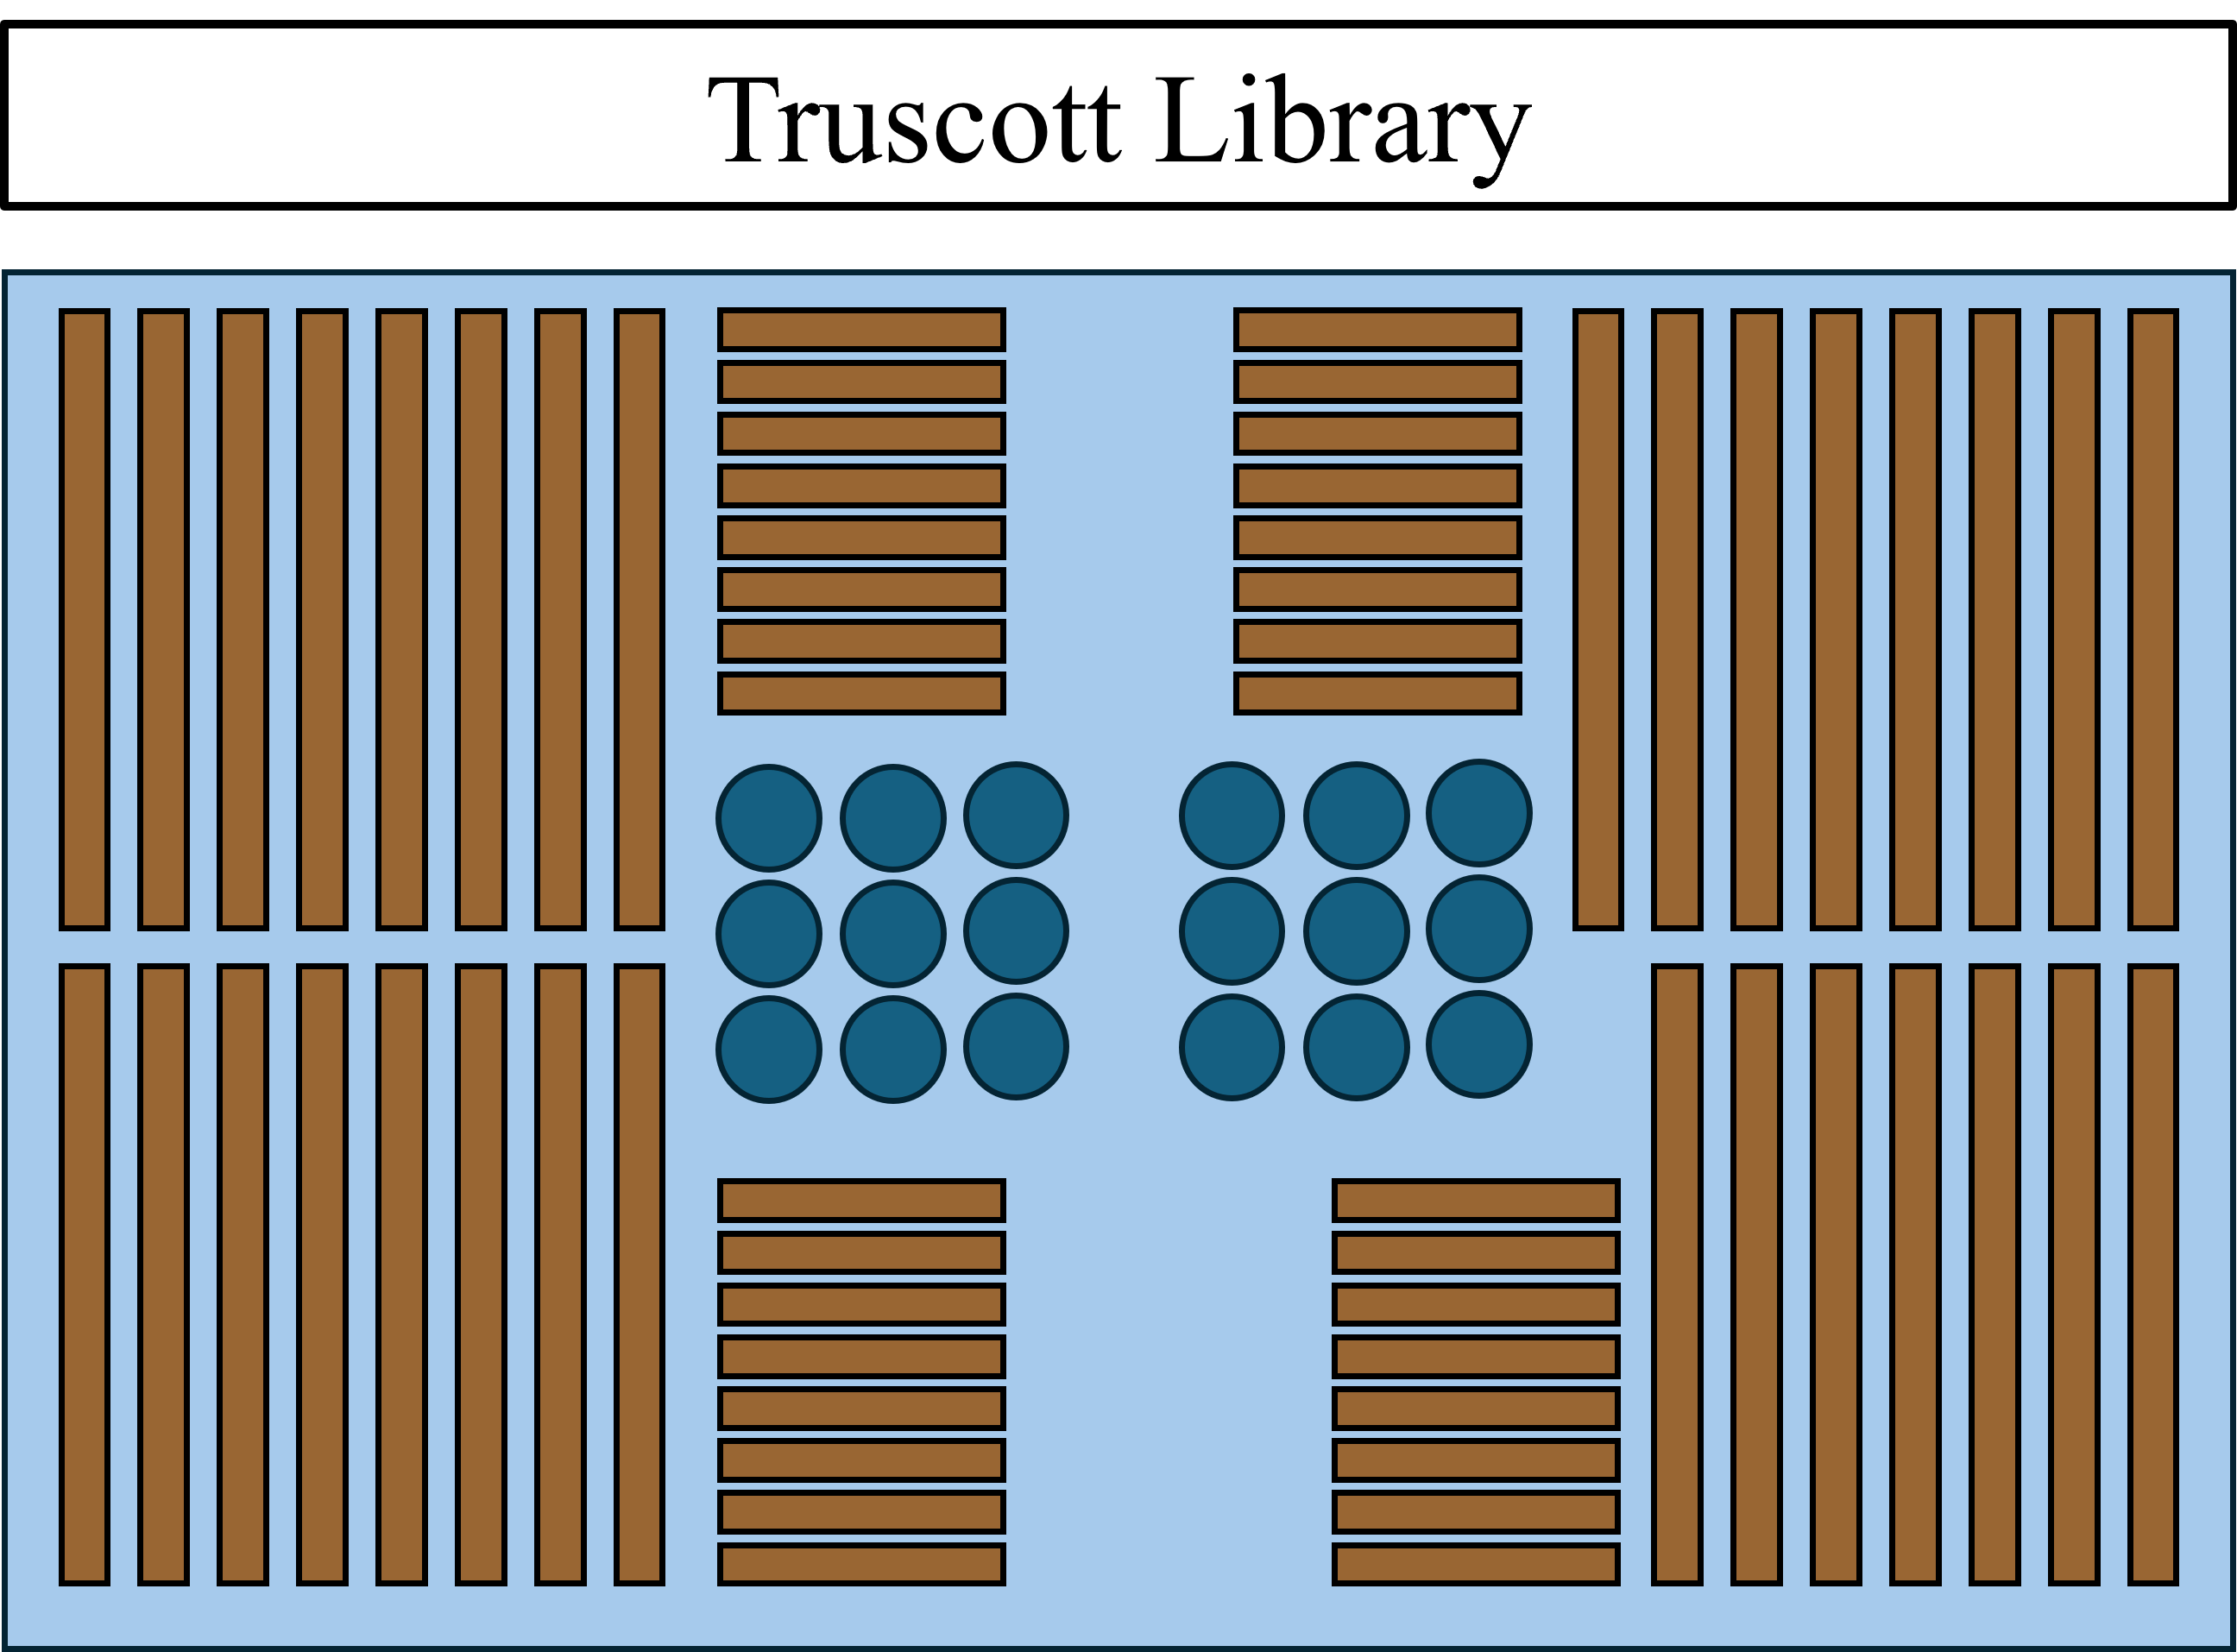
\includegraphics[width=0.55\textwidth]{../supplemental_materials/library_2.png}
\end{figure}
\end{frame}

\begin{frame}{Library Analogy (Cont.)}
\phantomsection\label{library-analogy-cont.-2}
\begin{figure}
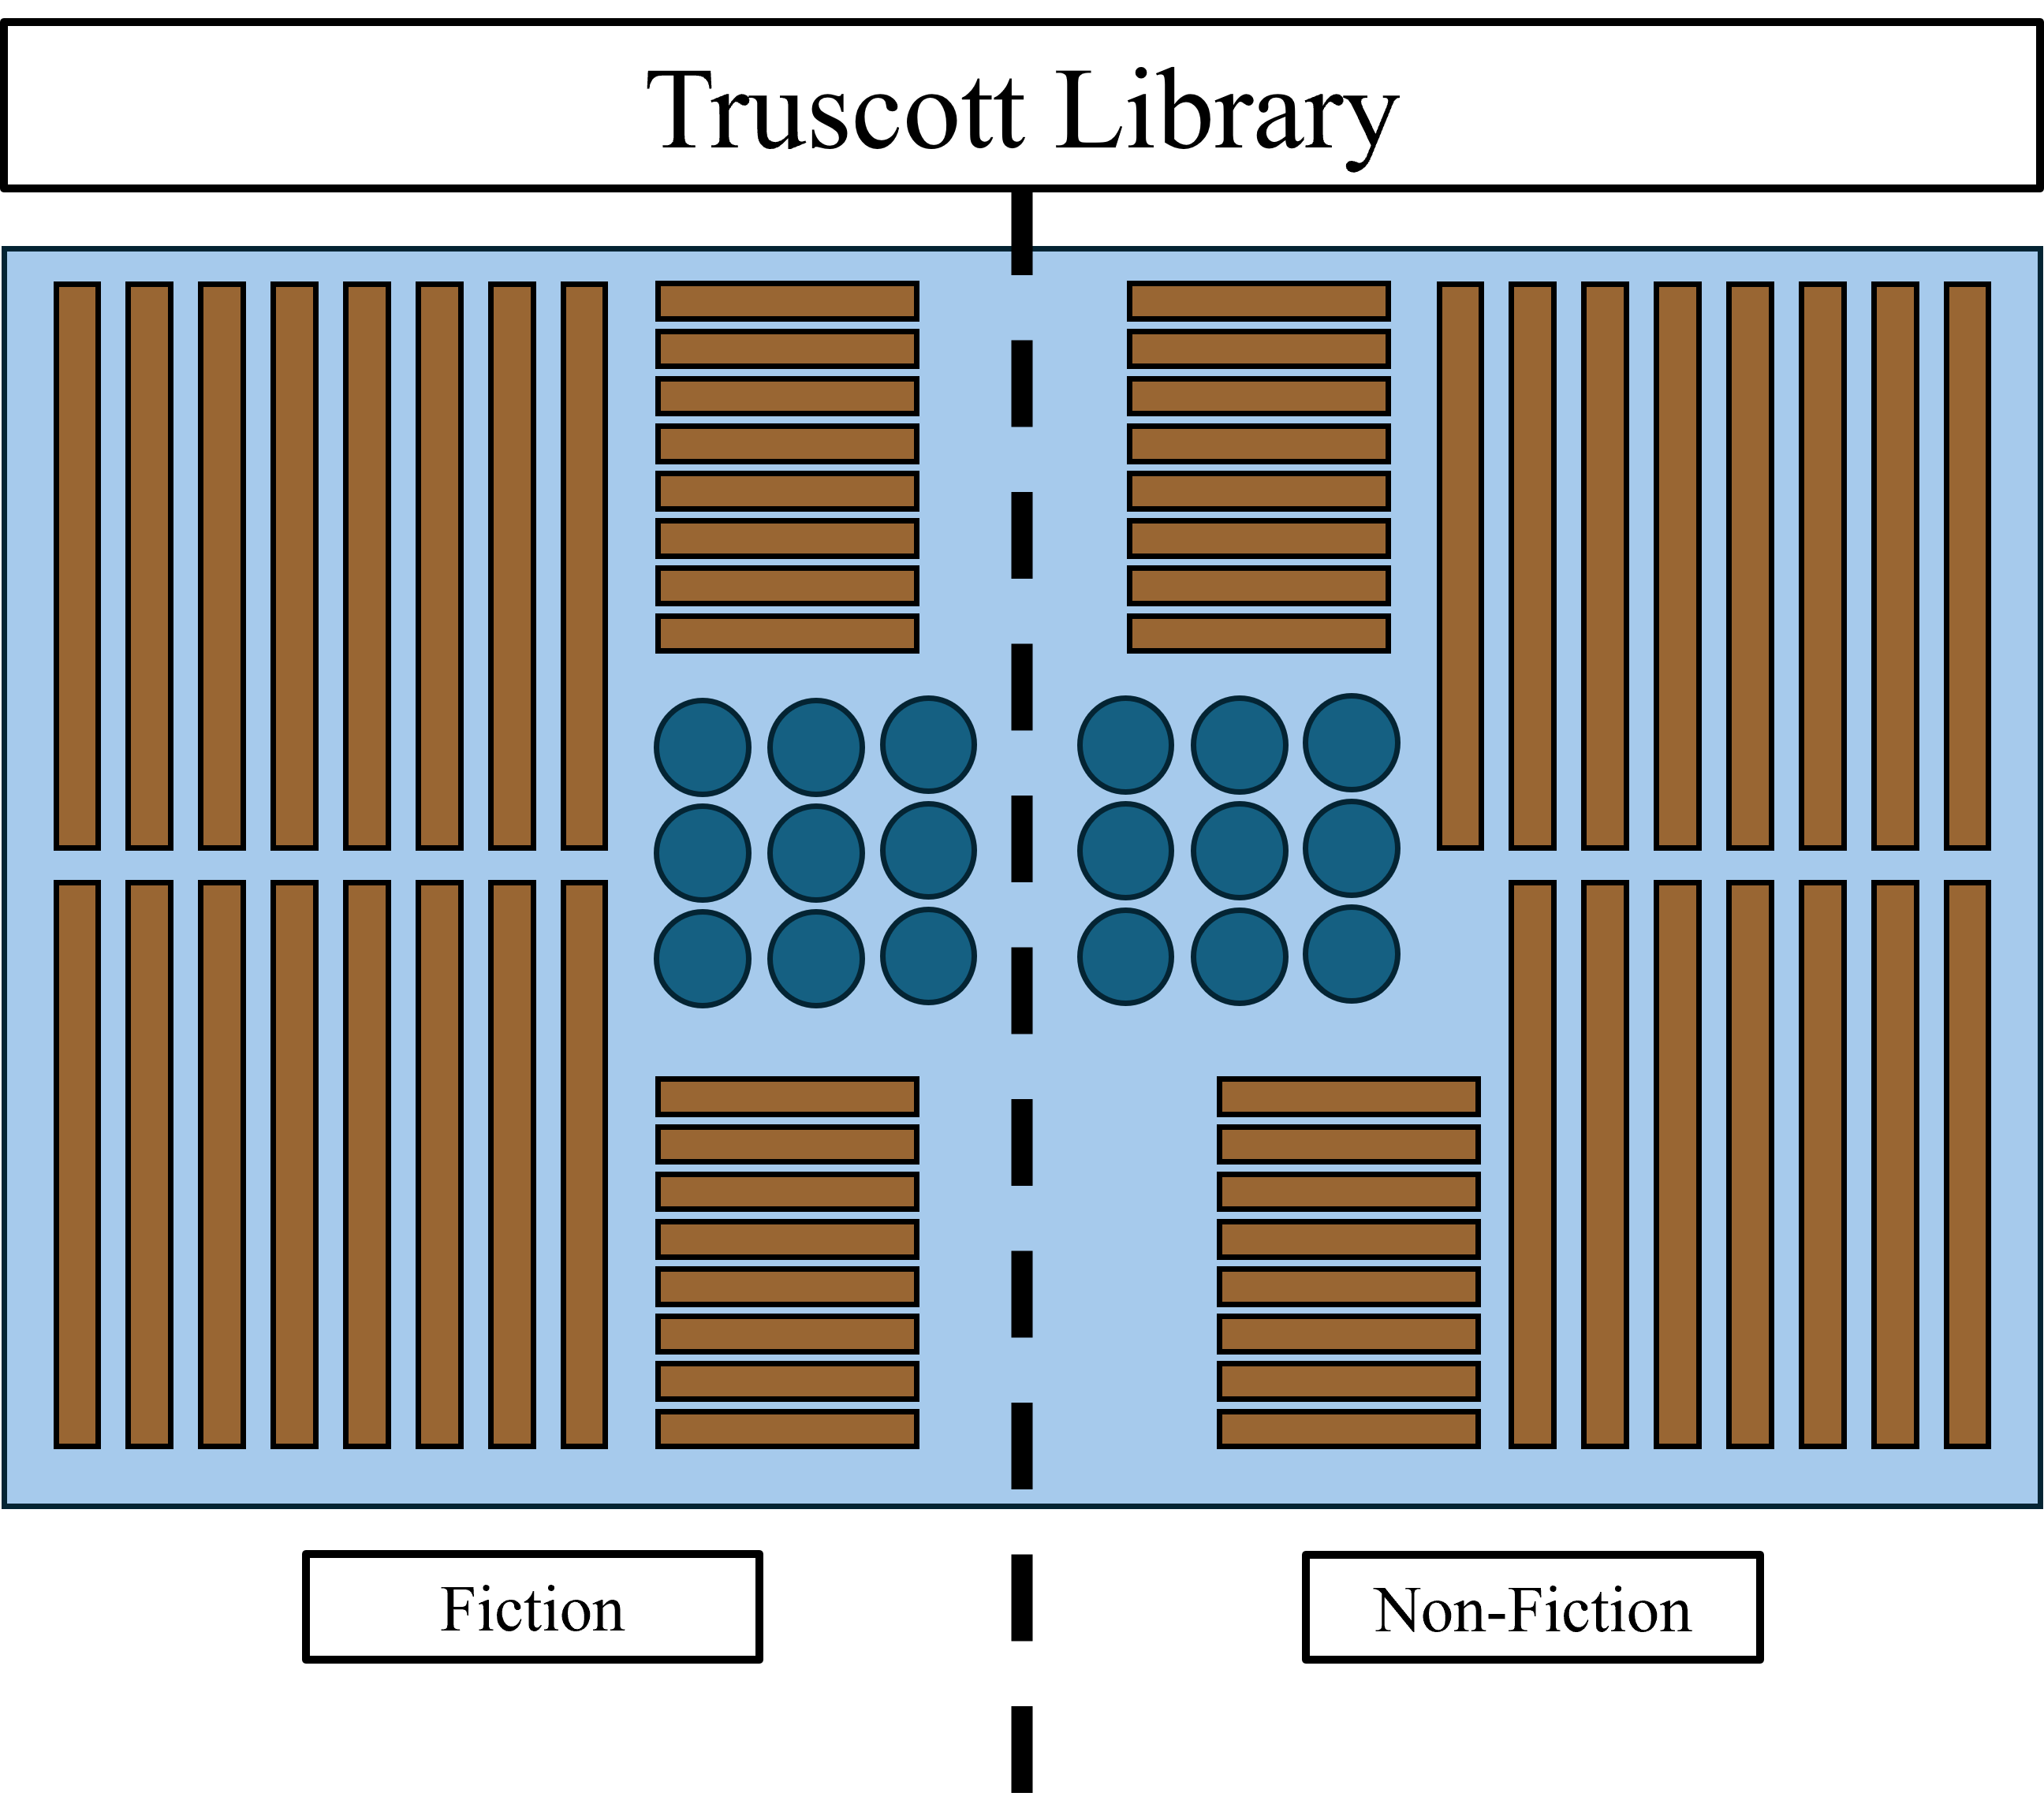
\includegraphics[width=0.55\textwidth]{../supplemental_materials/library_3.png}
\end{figure}
\end{frame}

\begin{frame}{Library Analogy (Cont.)}
\phantomsection\label{library-analogy-cont.-3}
\begin{figure}
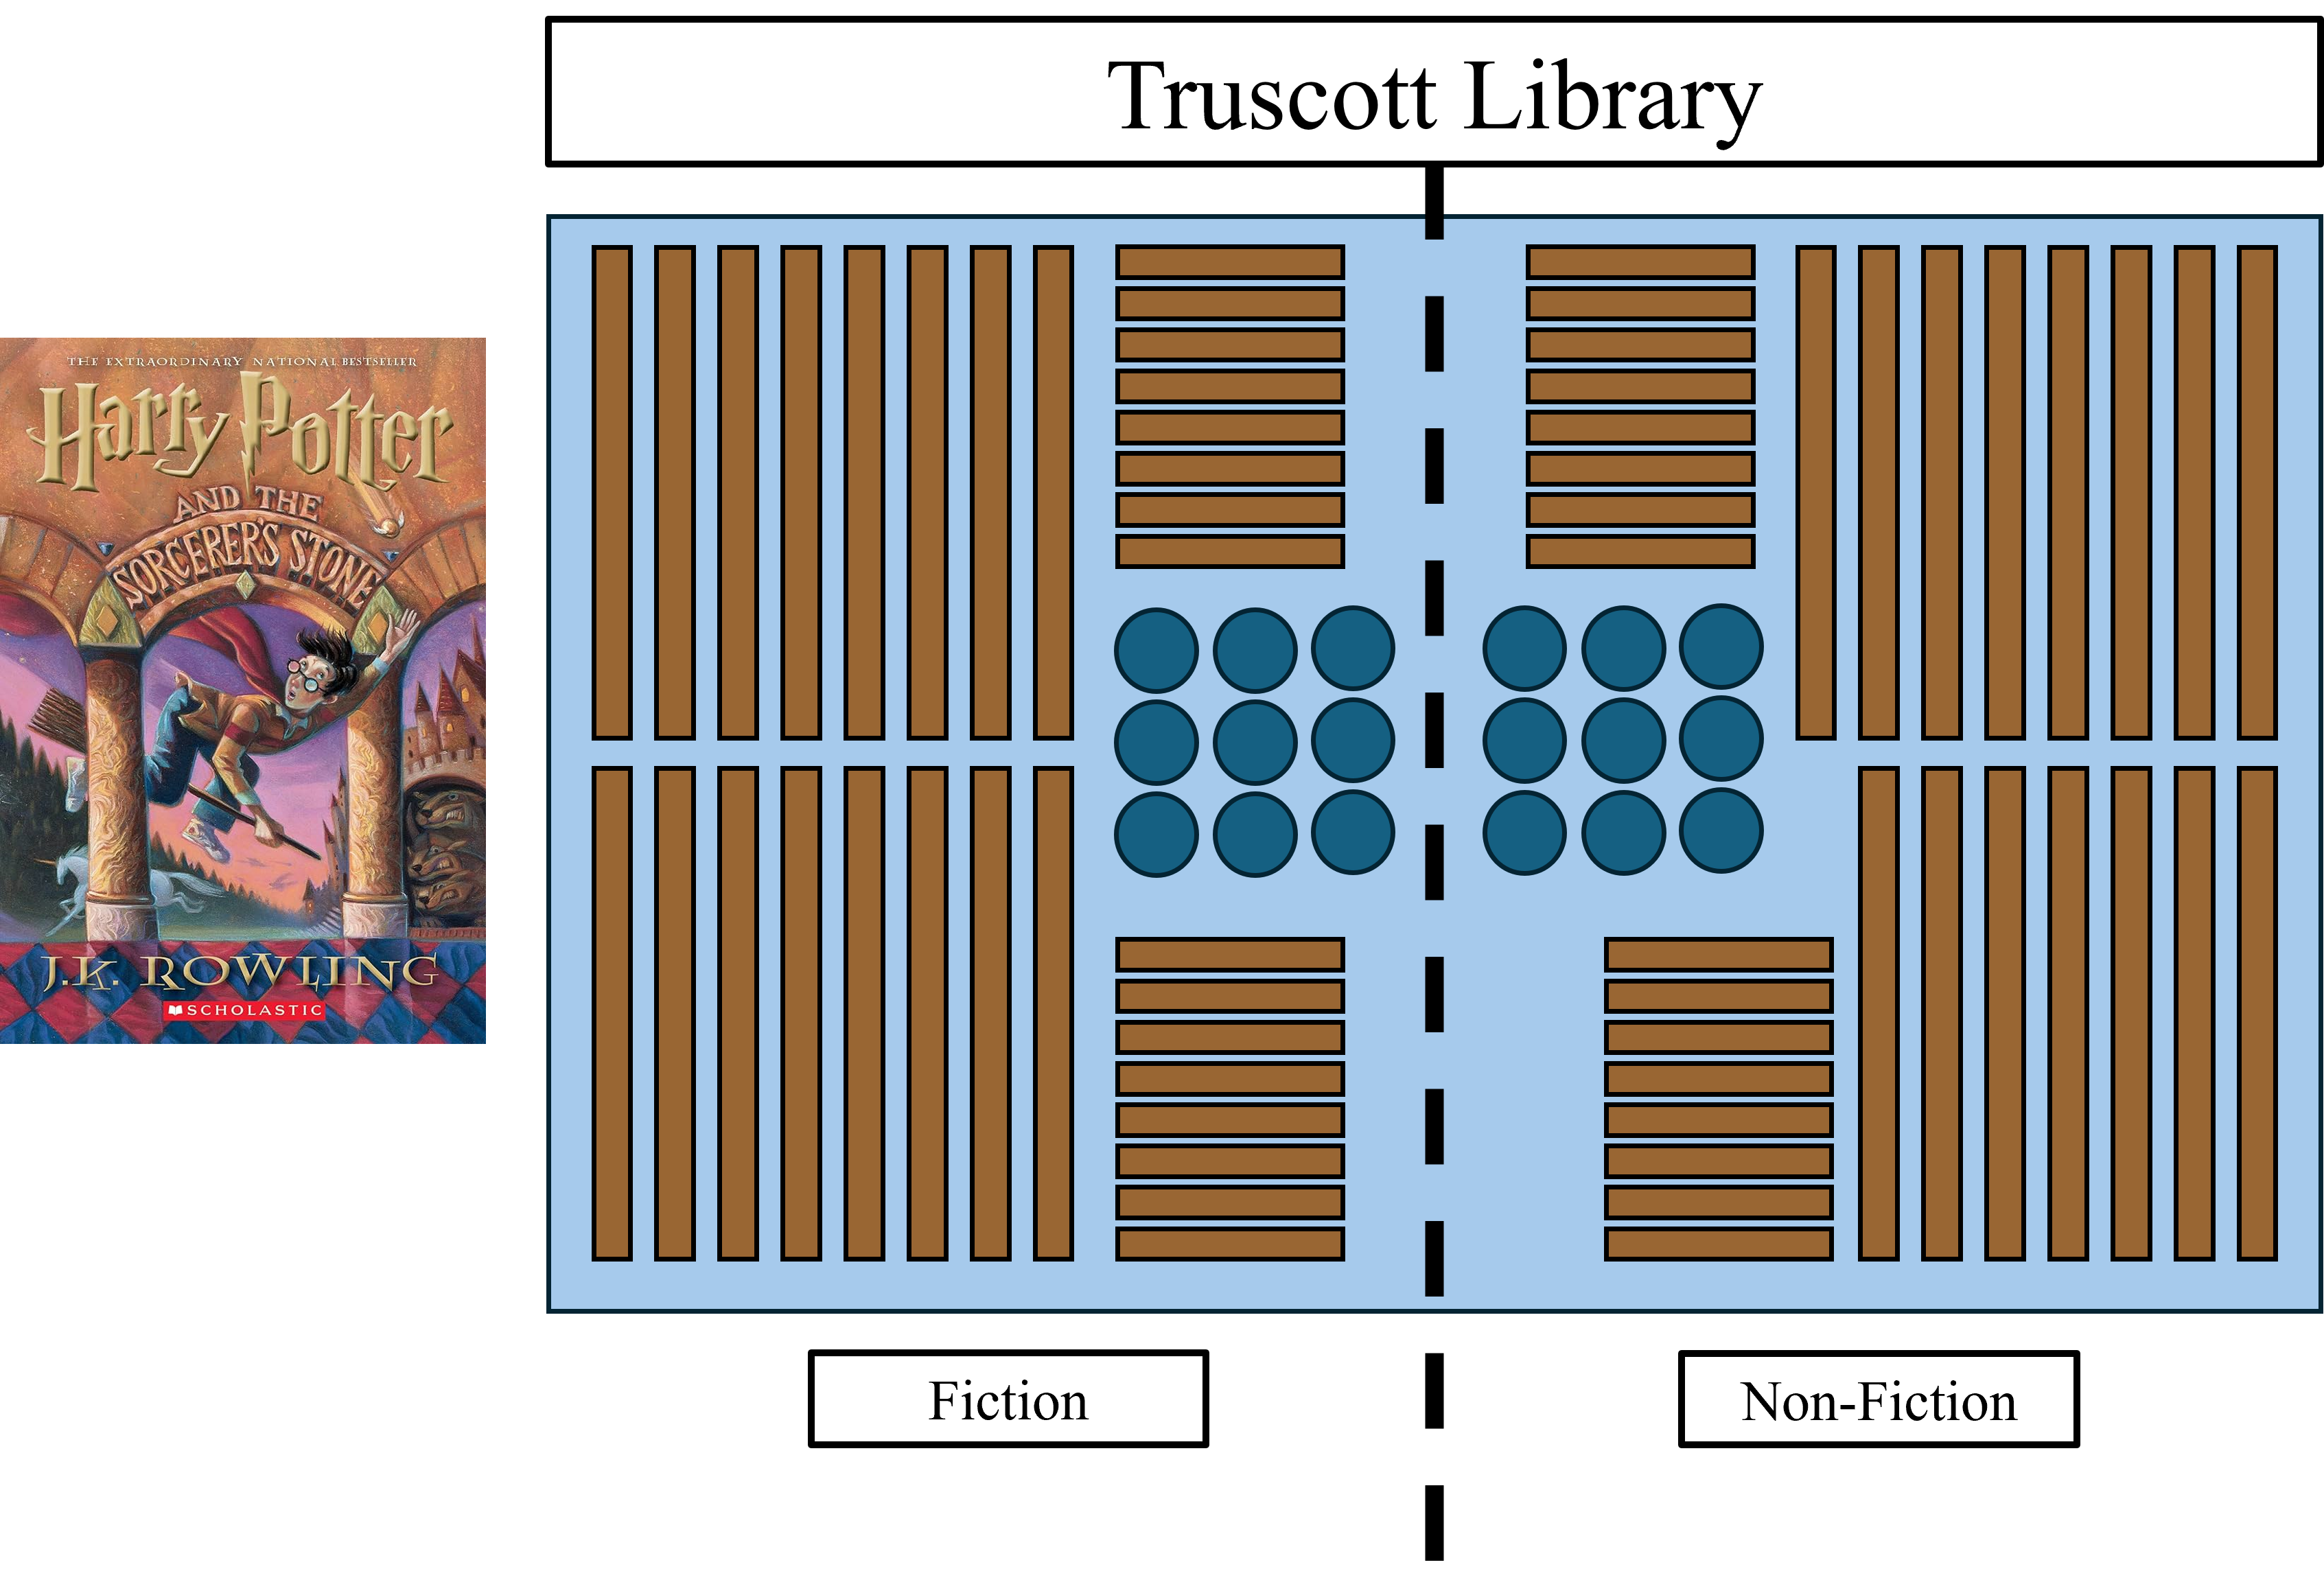
\includegraphics[width=0.55\textwidth]{../supplemental_materials/library_4.png}
\end{figure}
\end{frame}

\begin{frame}{Library Analogy (Cont.)}
\phantomsection\label{library-analogy-cont.-4}
\begin{figure}
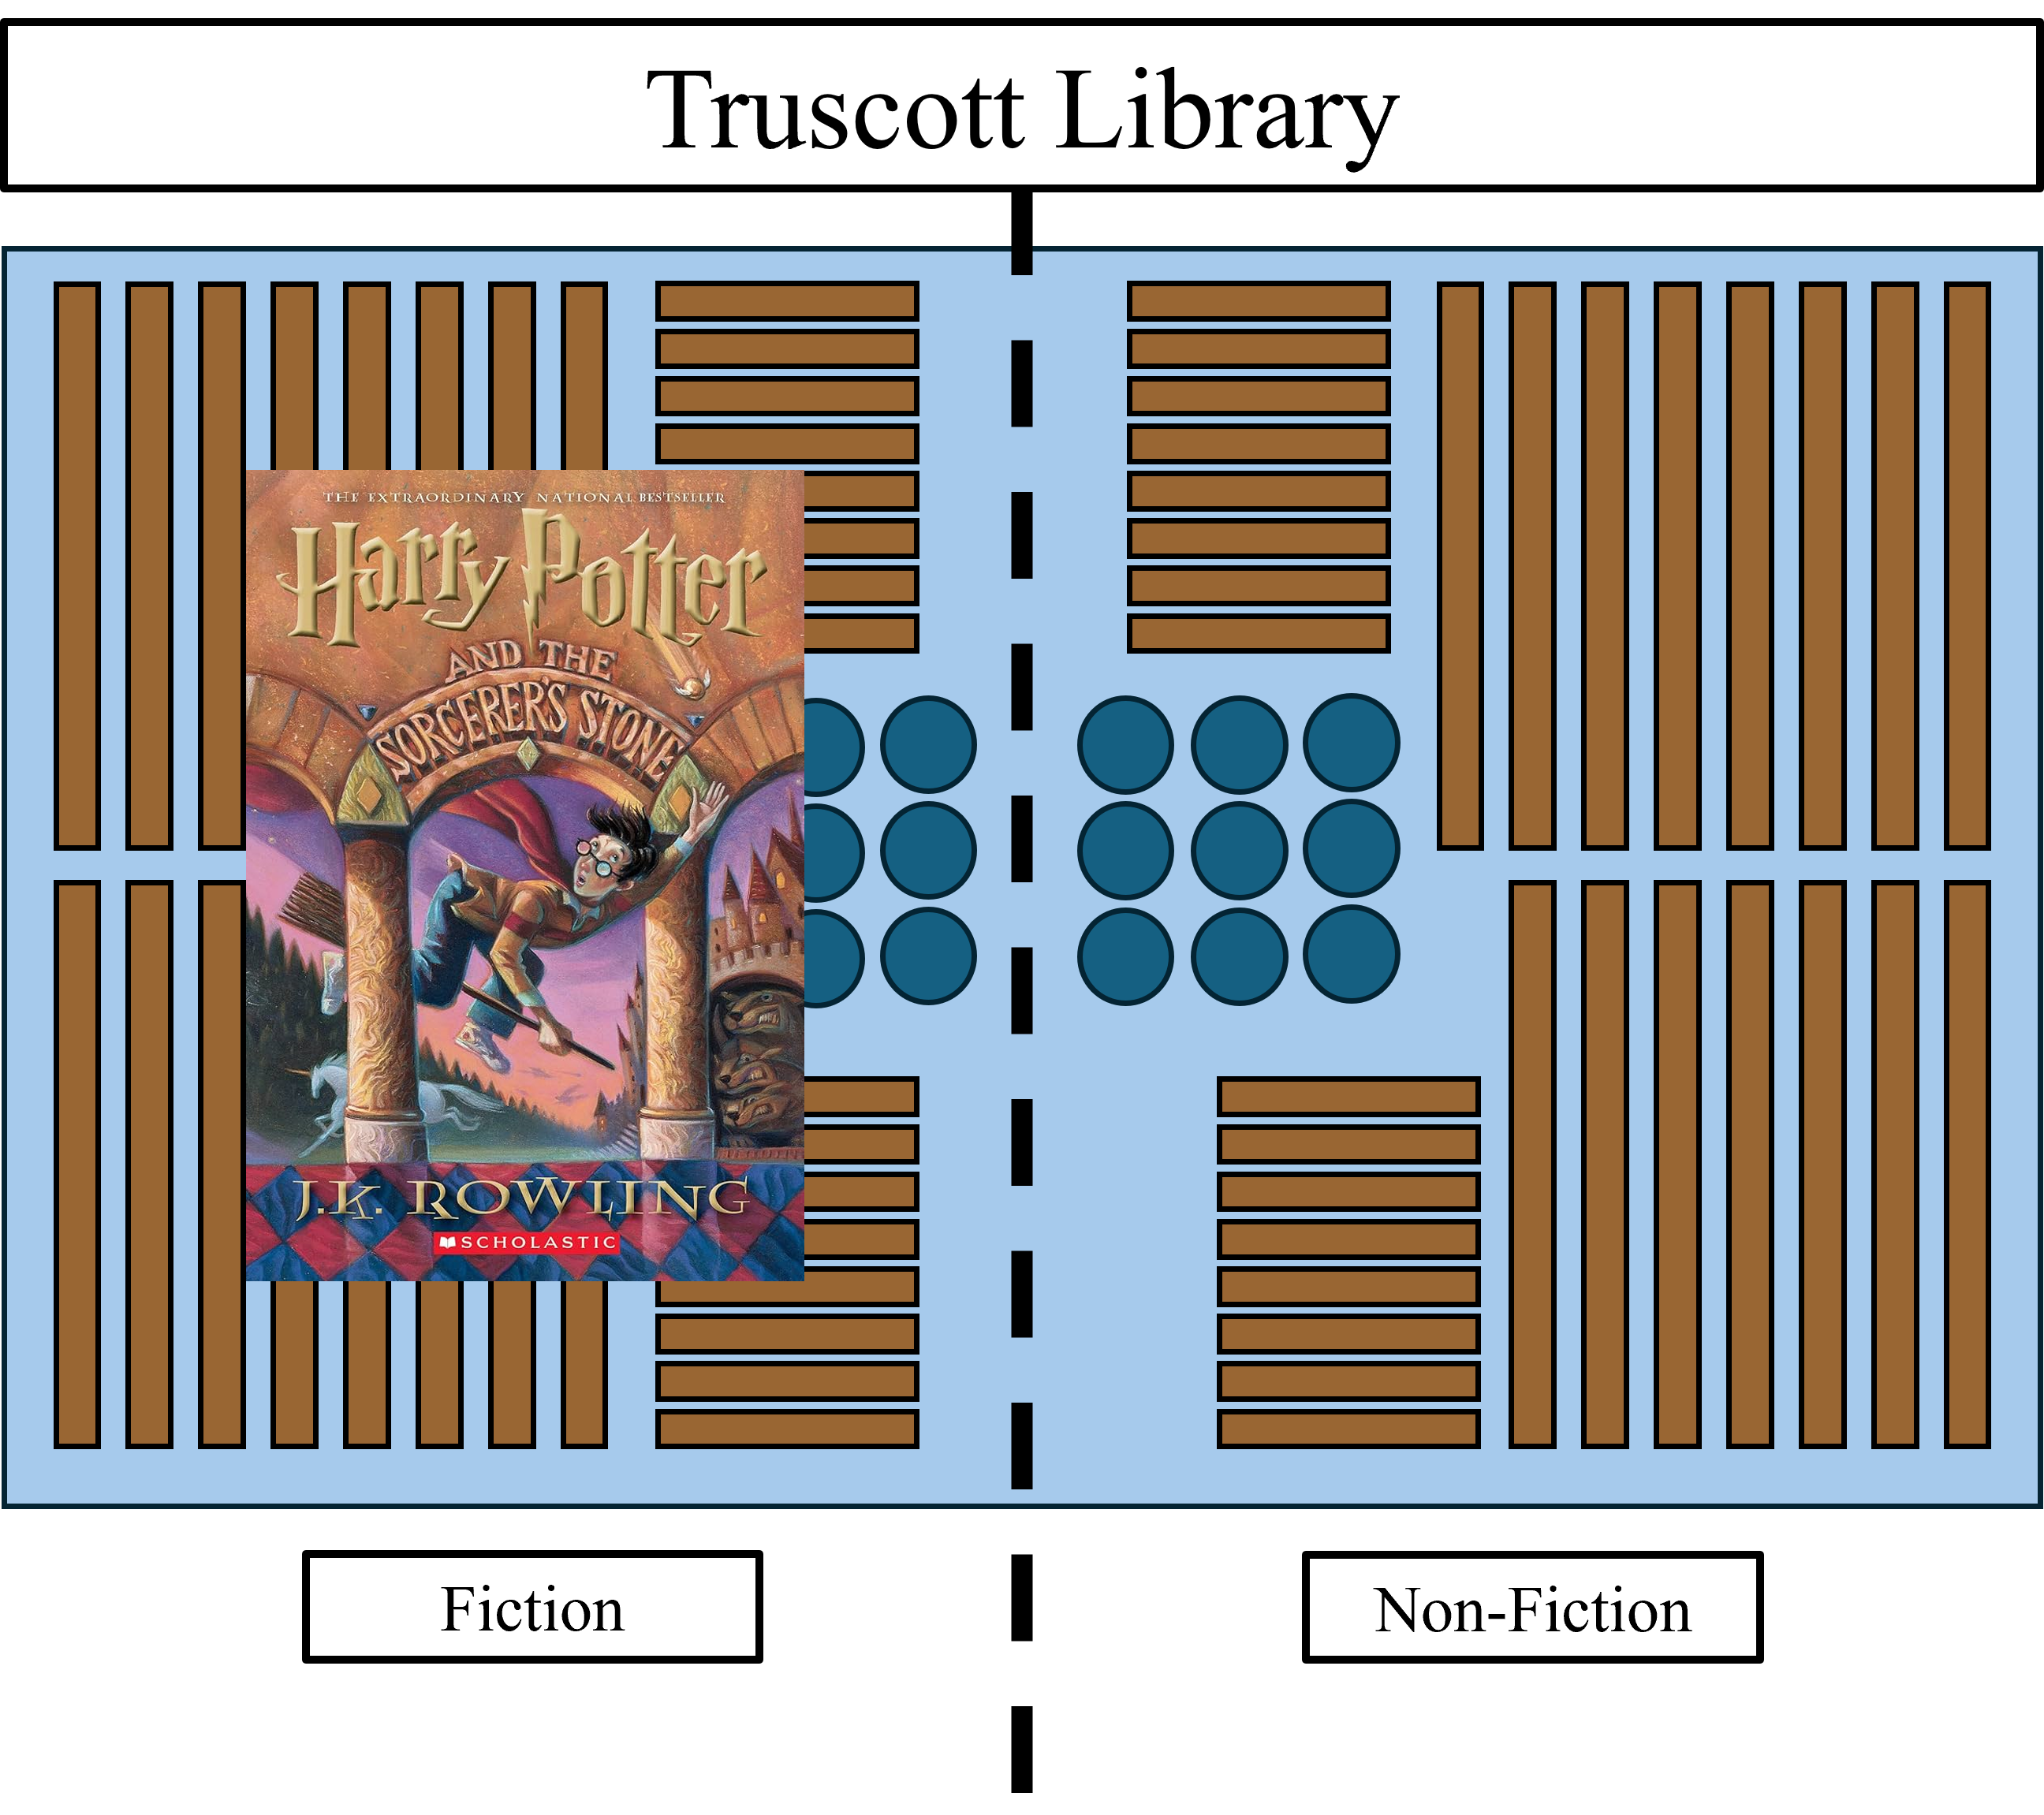
\includegraphics[width=0.55\textwidth]{../supplemental_materials/library_4.1.png}
\end{figure}
\end{frame}

\begin{frame}{Library Analogy (Cont.)}
\phantomsection\label{library-analogy-cont.-5}
\begin{figure}
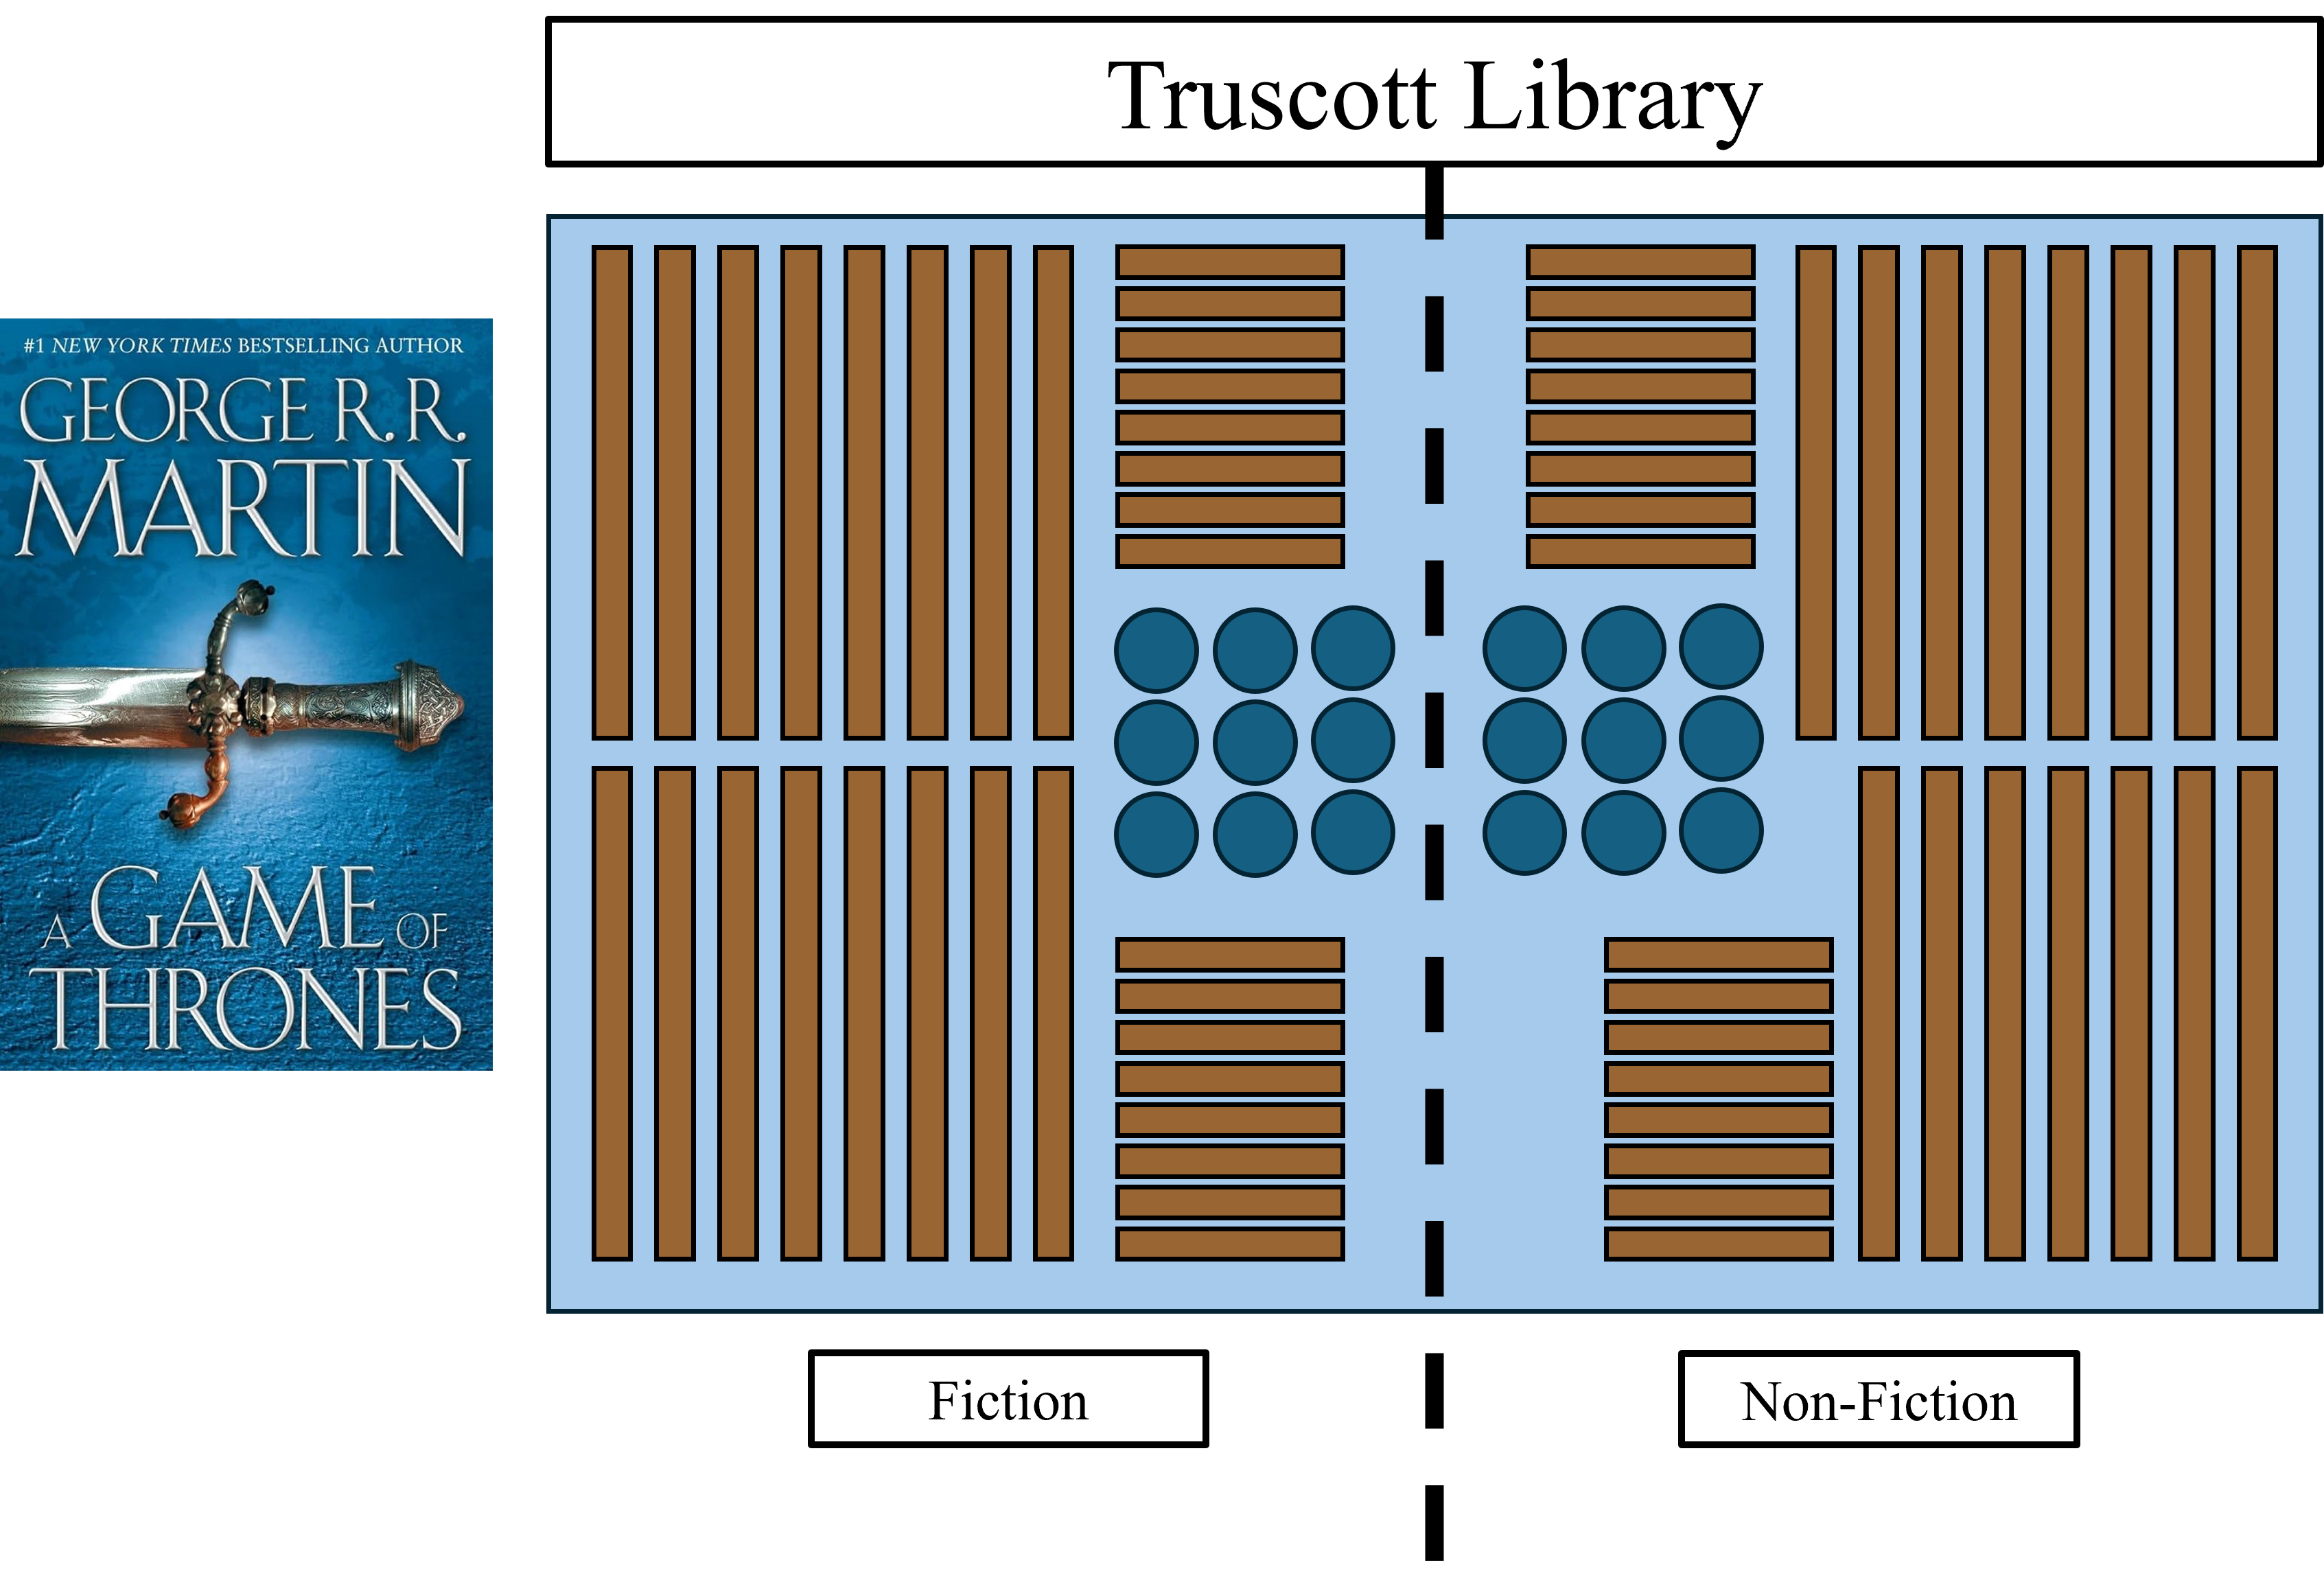
\includegraphics[width=0.55\textwidth]{../supplemental_materials/library_4_B.png}
\end{figure}
\end{frame}

\begin{frame}{Library Analogy (Cont.)}
\phantomsection\label{library-analogy-cont.-6}
\begin{figure}
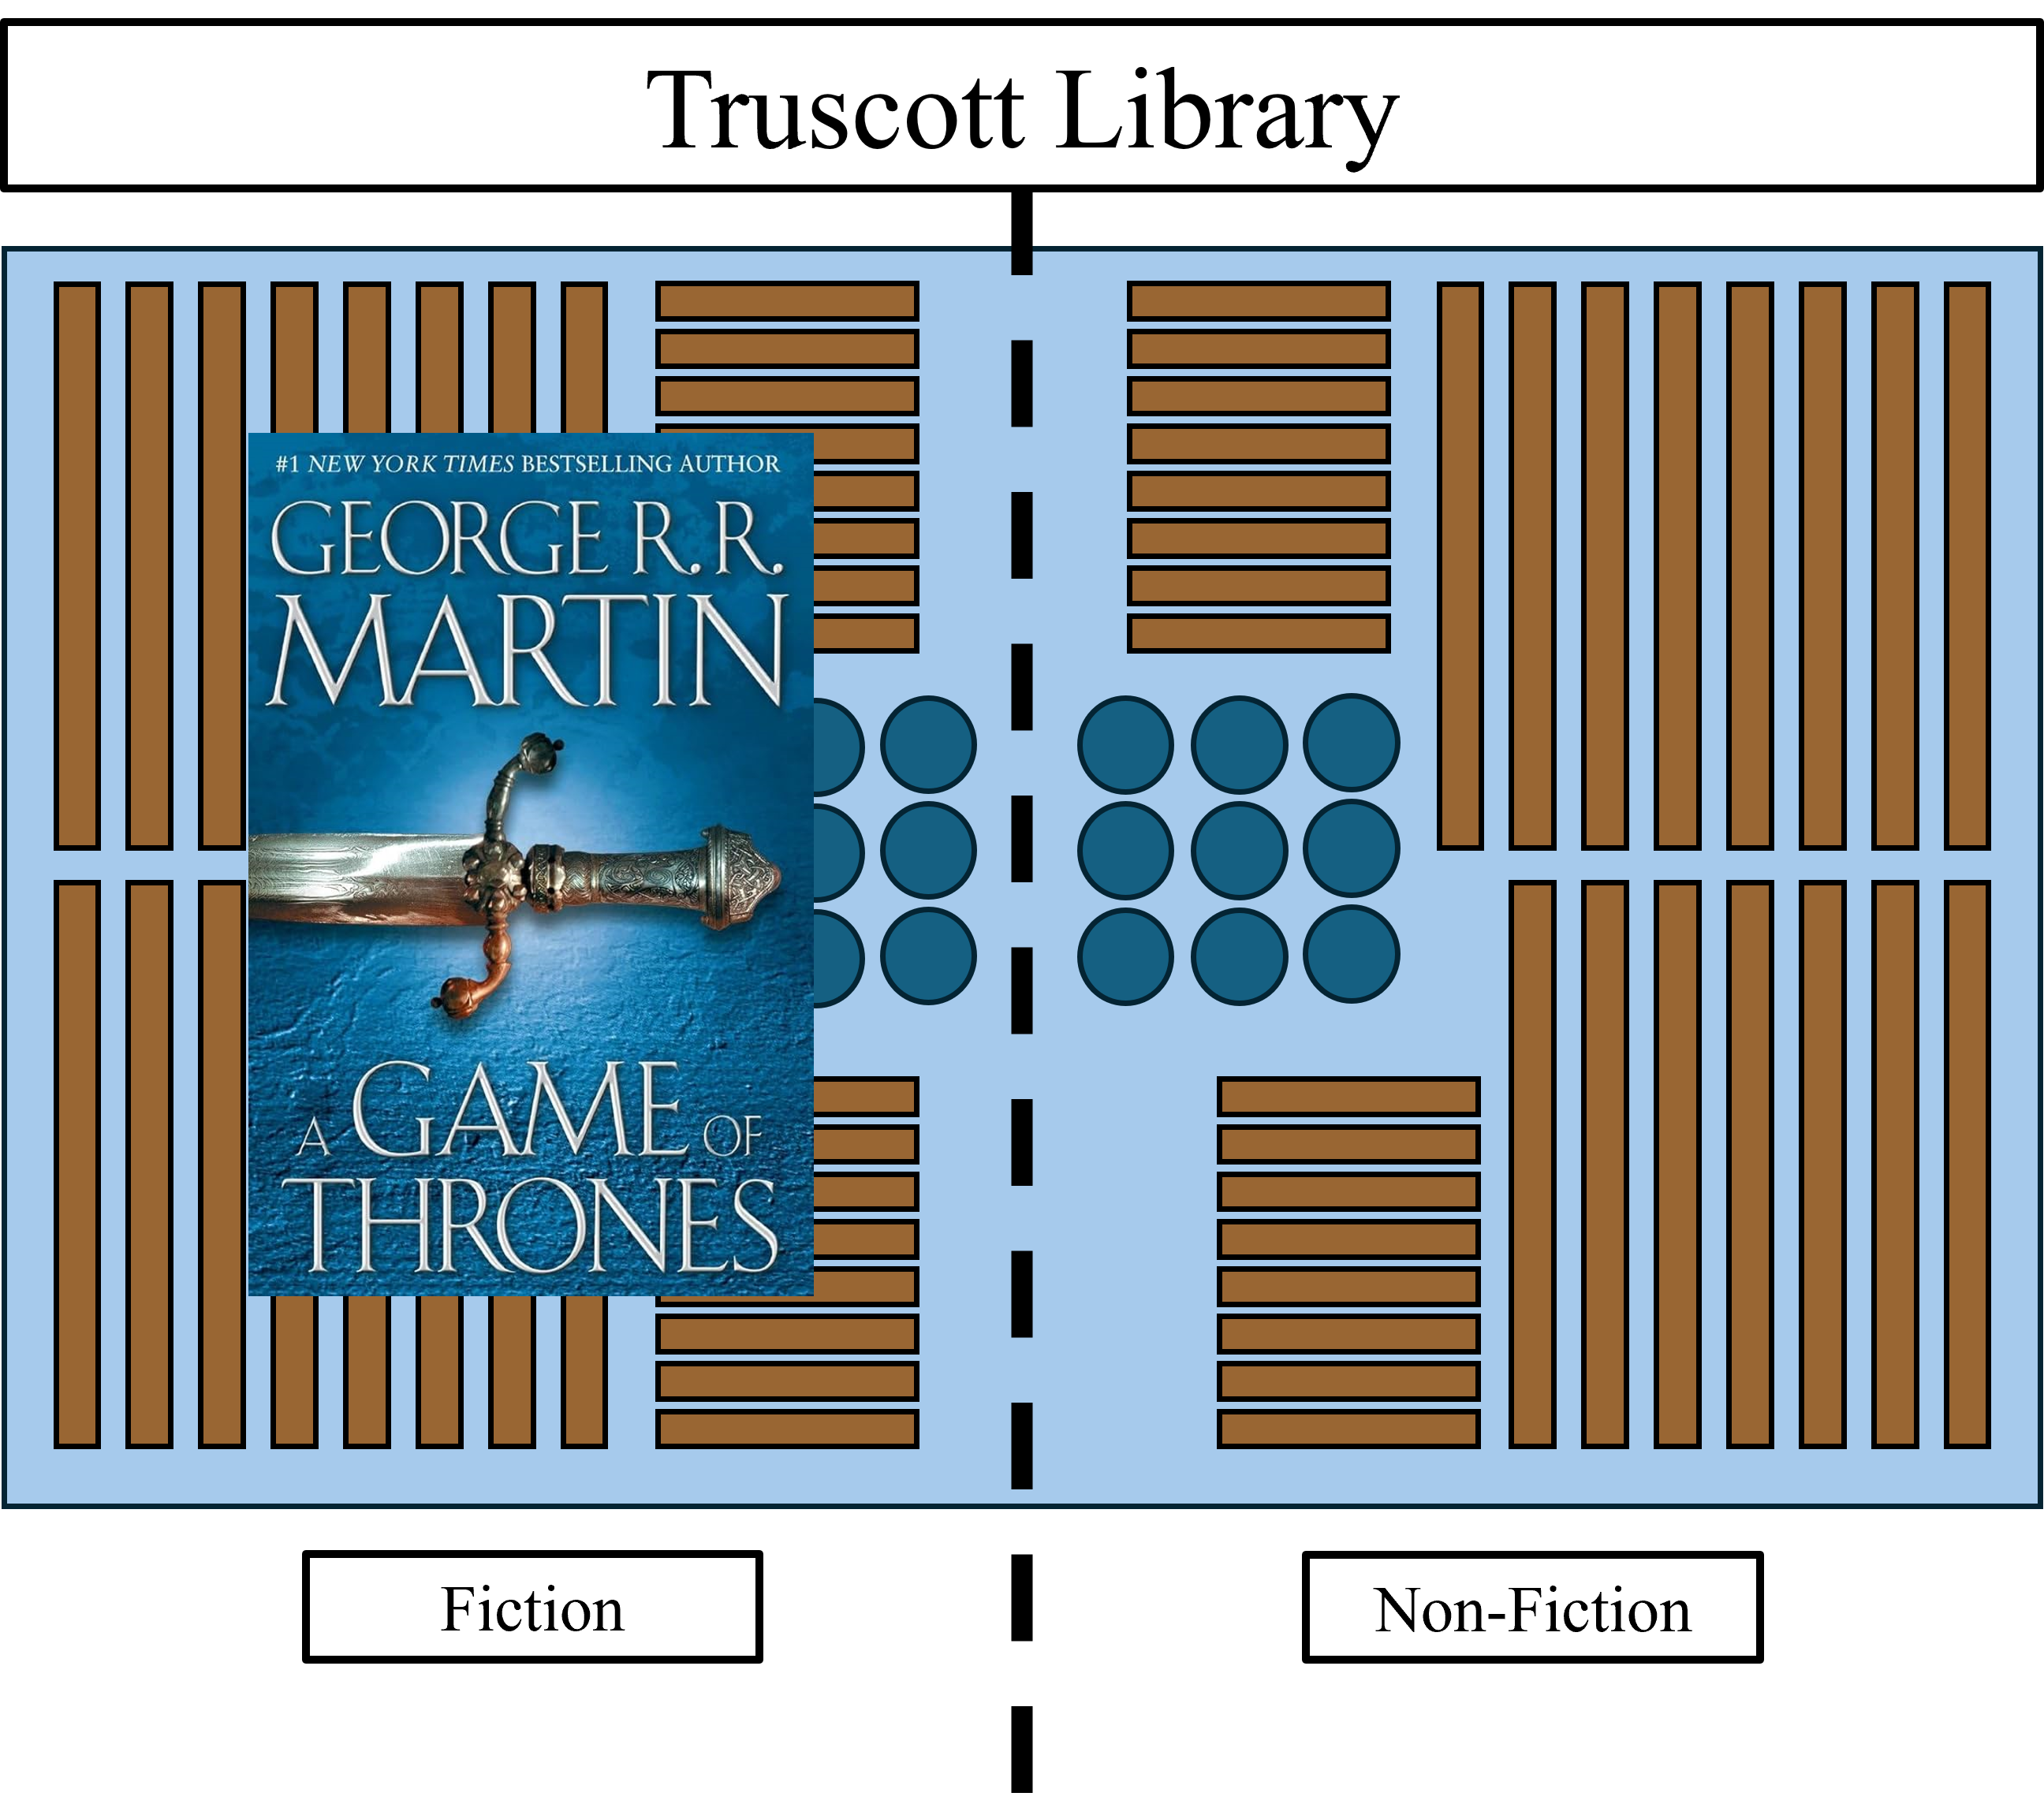
\includegraphics[width=0.55\textwidth]{../supplemental_materials/library_4_B.1.png}
\end{figure}
\end{frame}

\begin{frame}{Library Analogy (Cont.)}
\phantomsection\label{library-analogy-cont.-7}
\begin{figure}
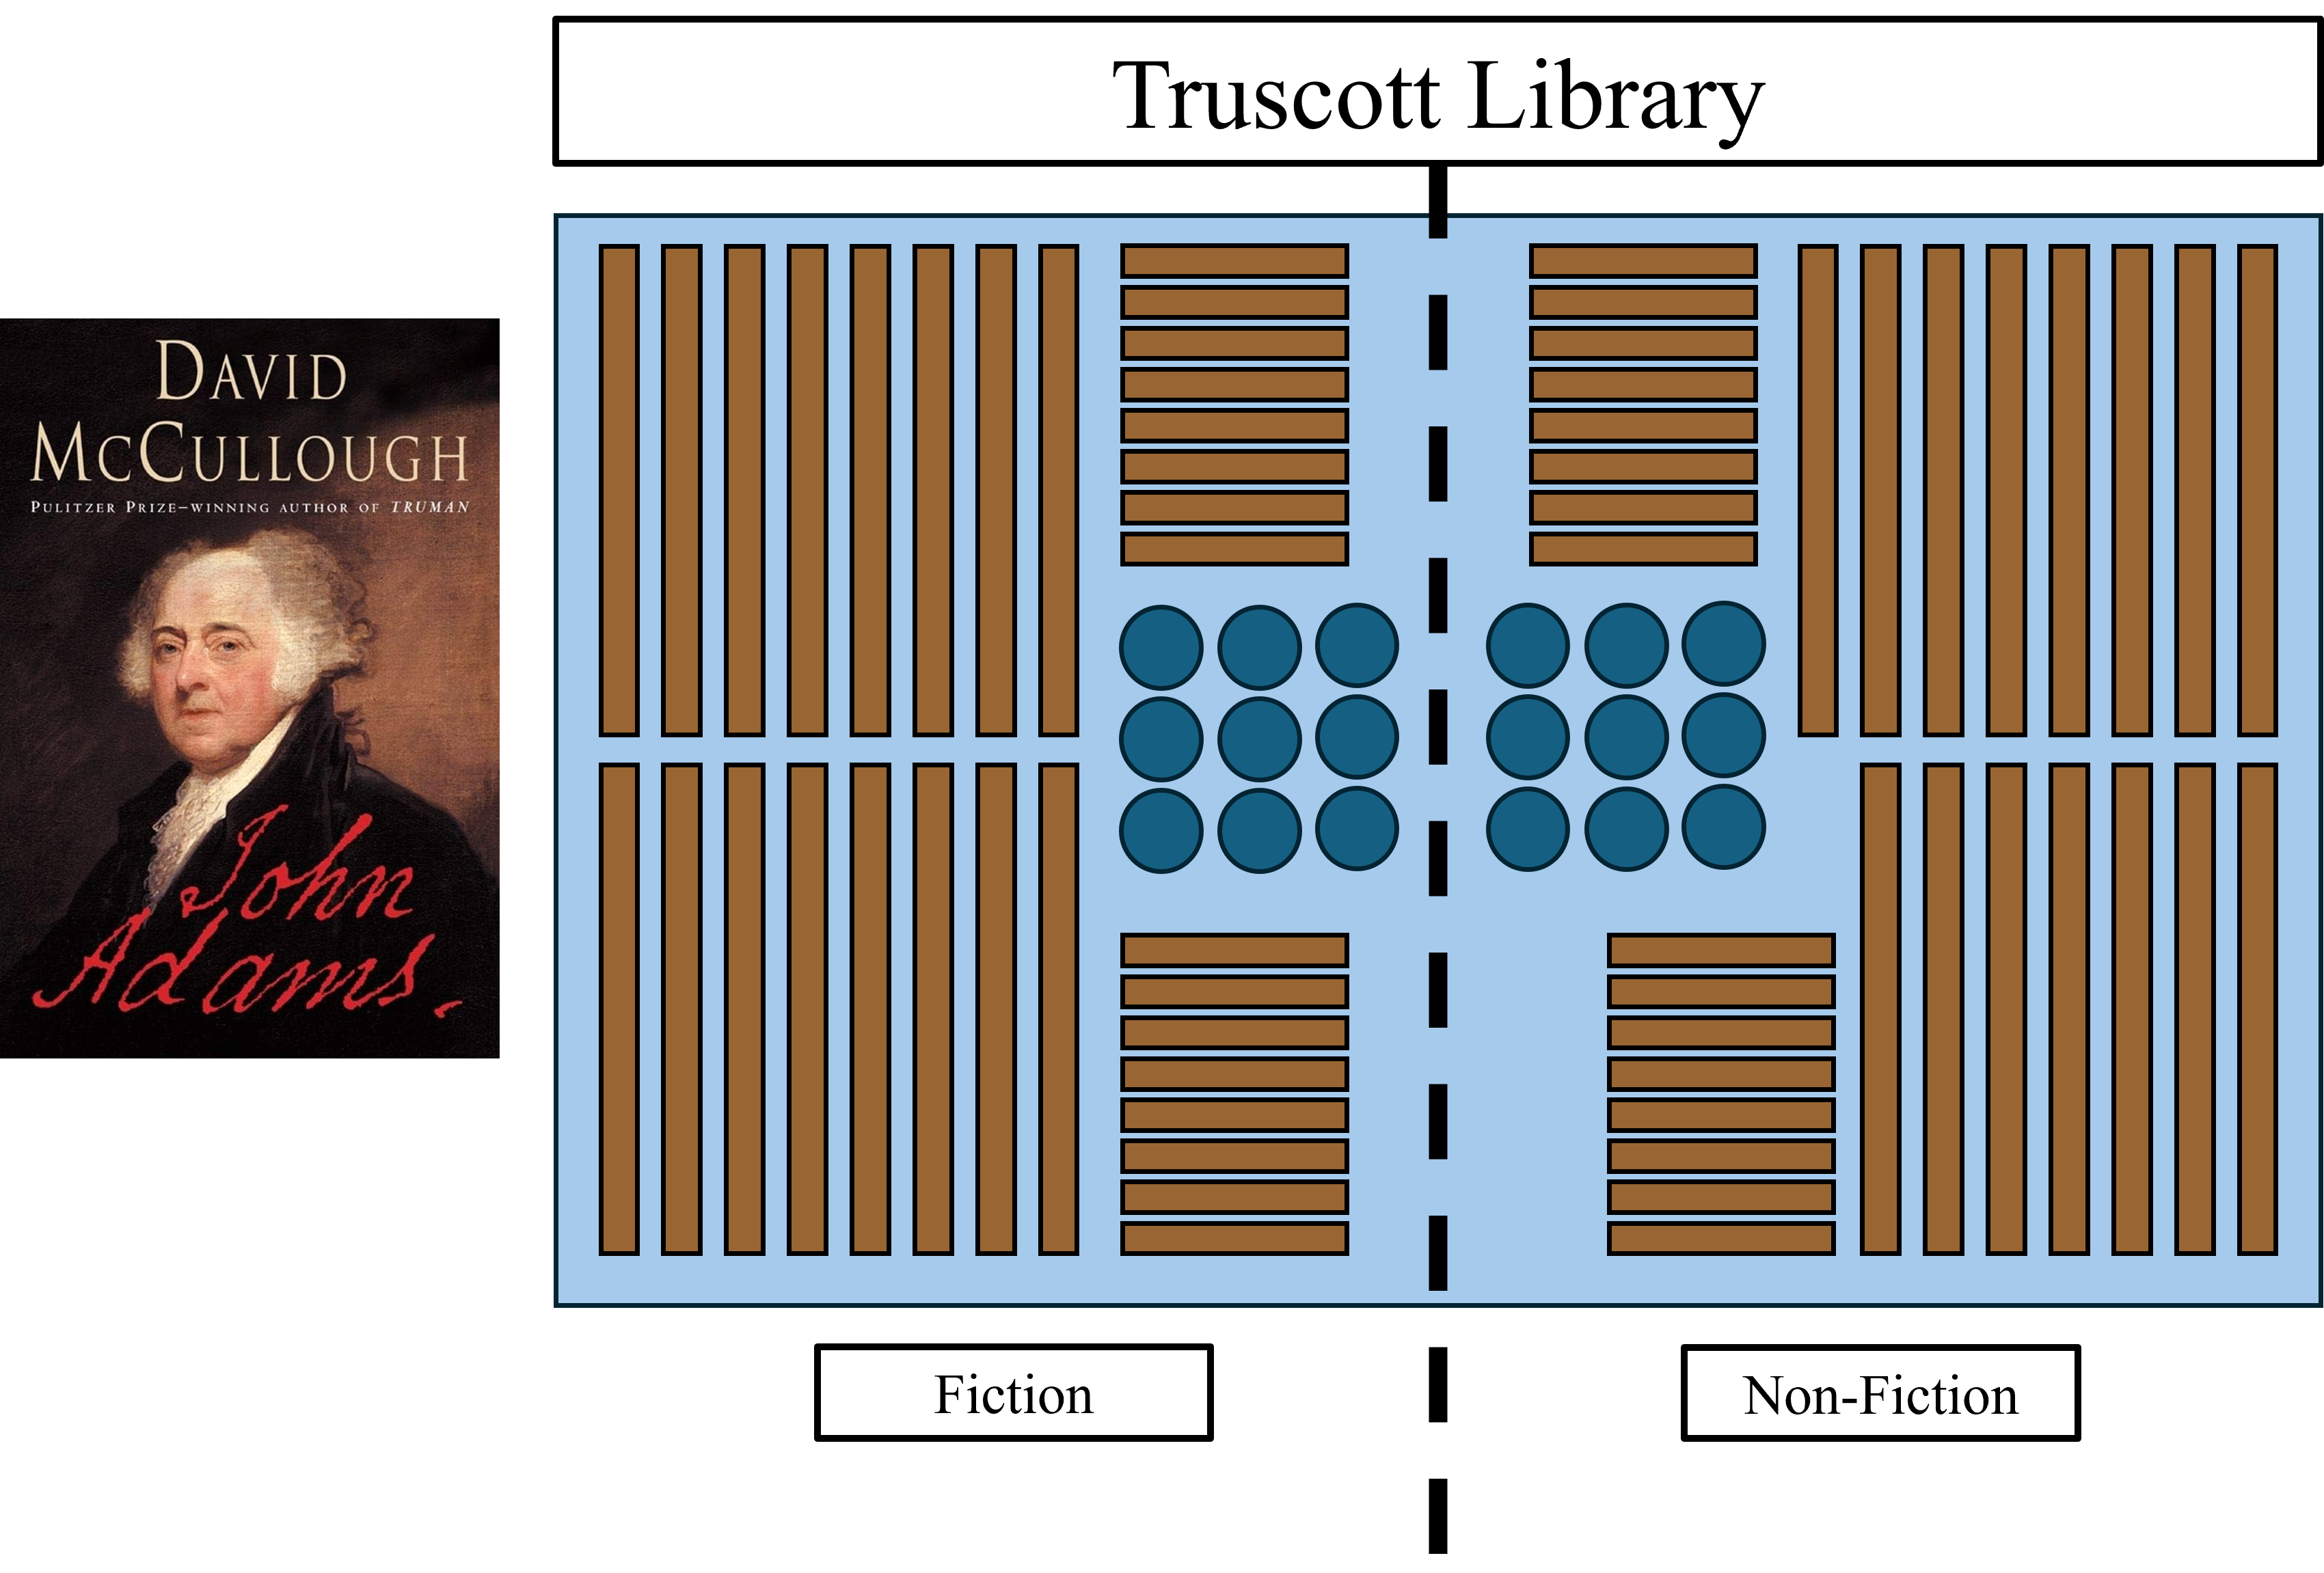
\includegraphics[width=0.55\textwidth]{../supplemental_materials/library_4_C.png}
\end{figure}
\end{frame}

\begin{frame}{Library Analogy (Cont.)}
\phantomsection\label{library-analogy-cont.-8}
\begin{figure}
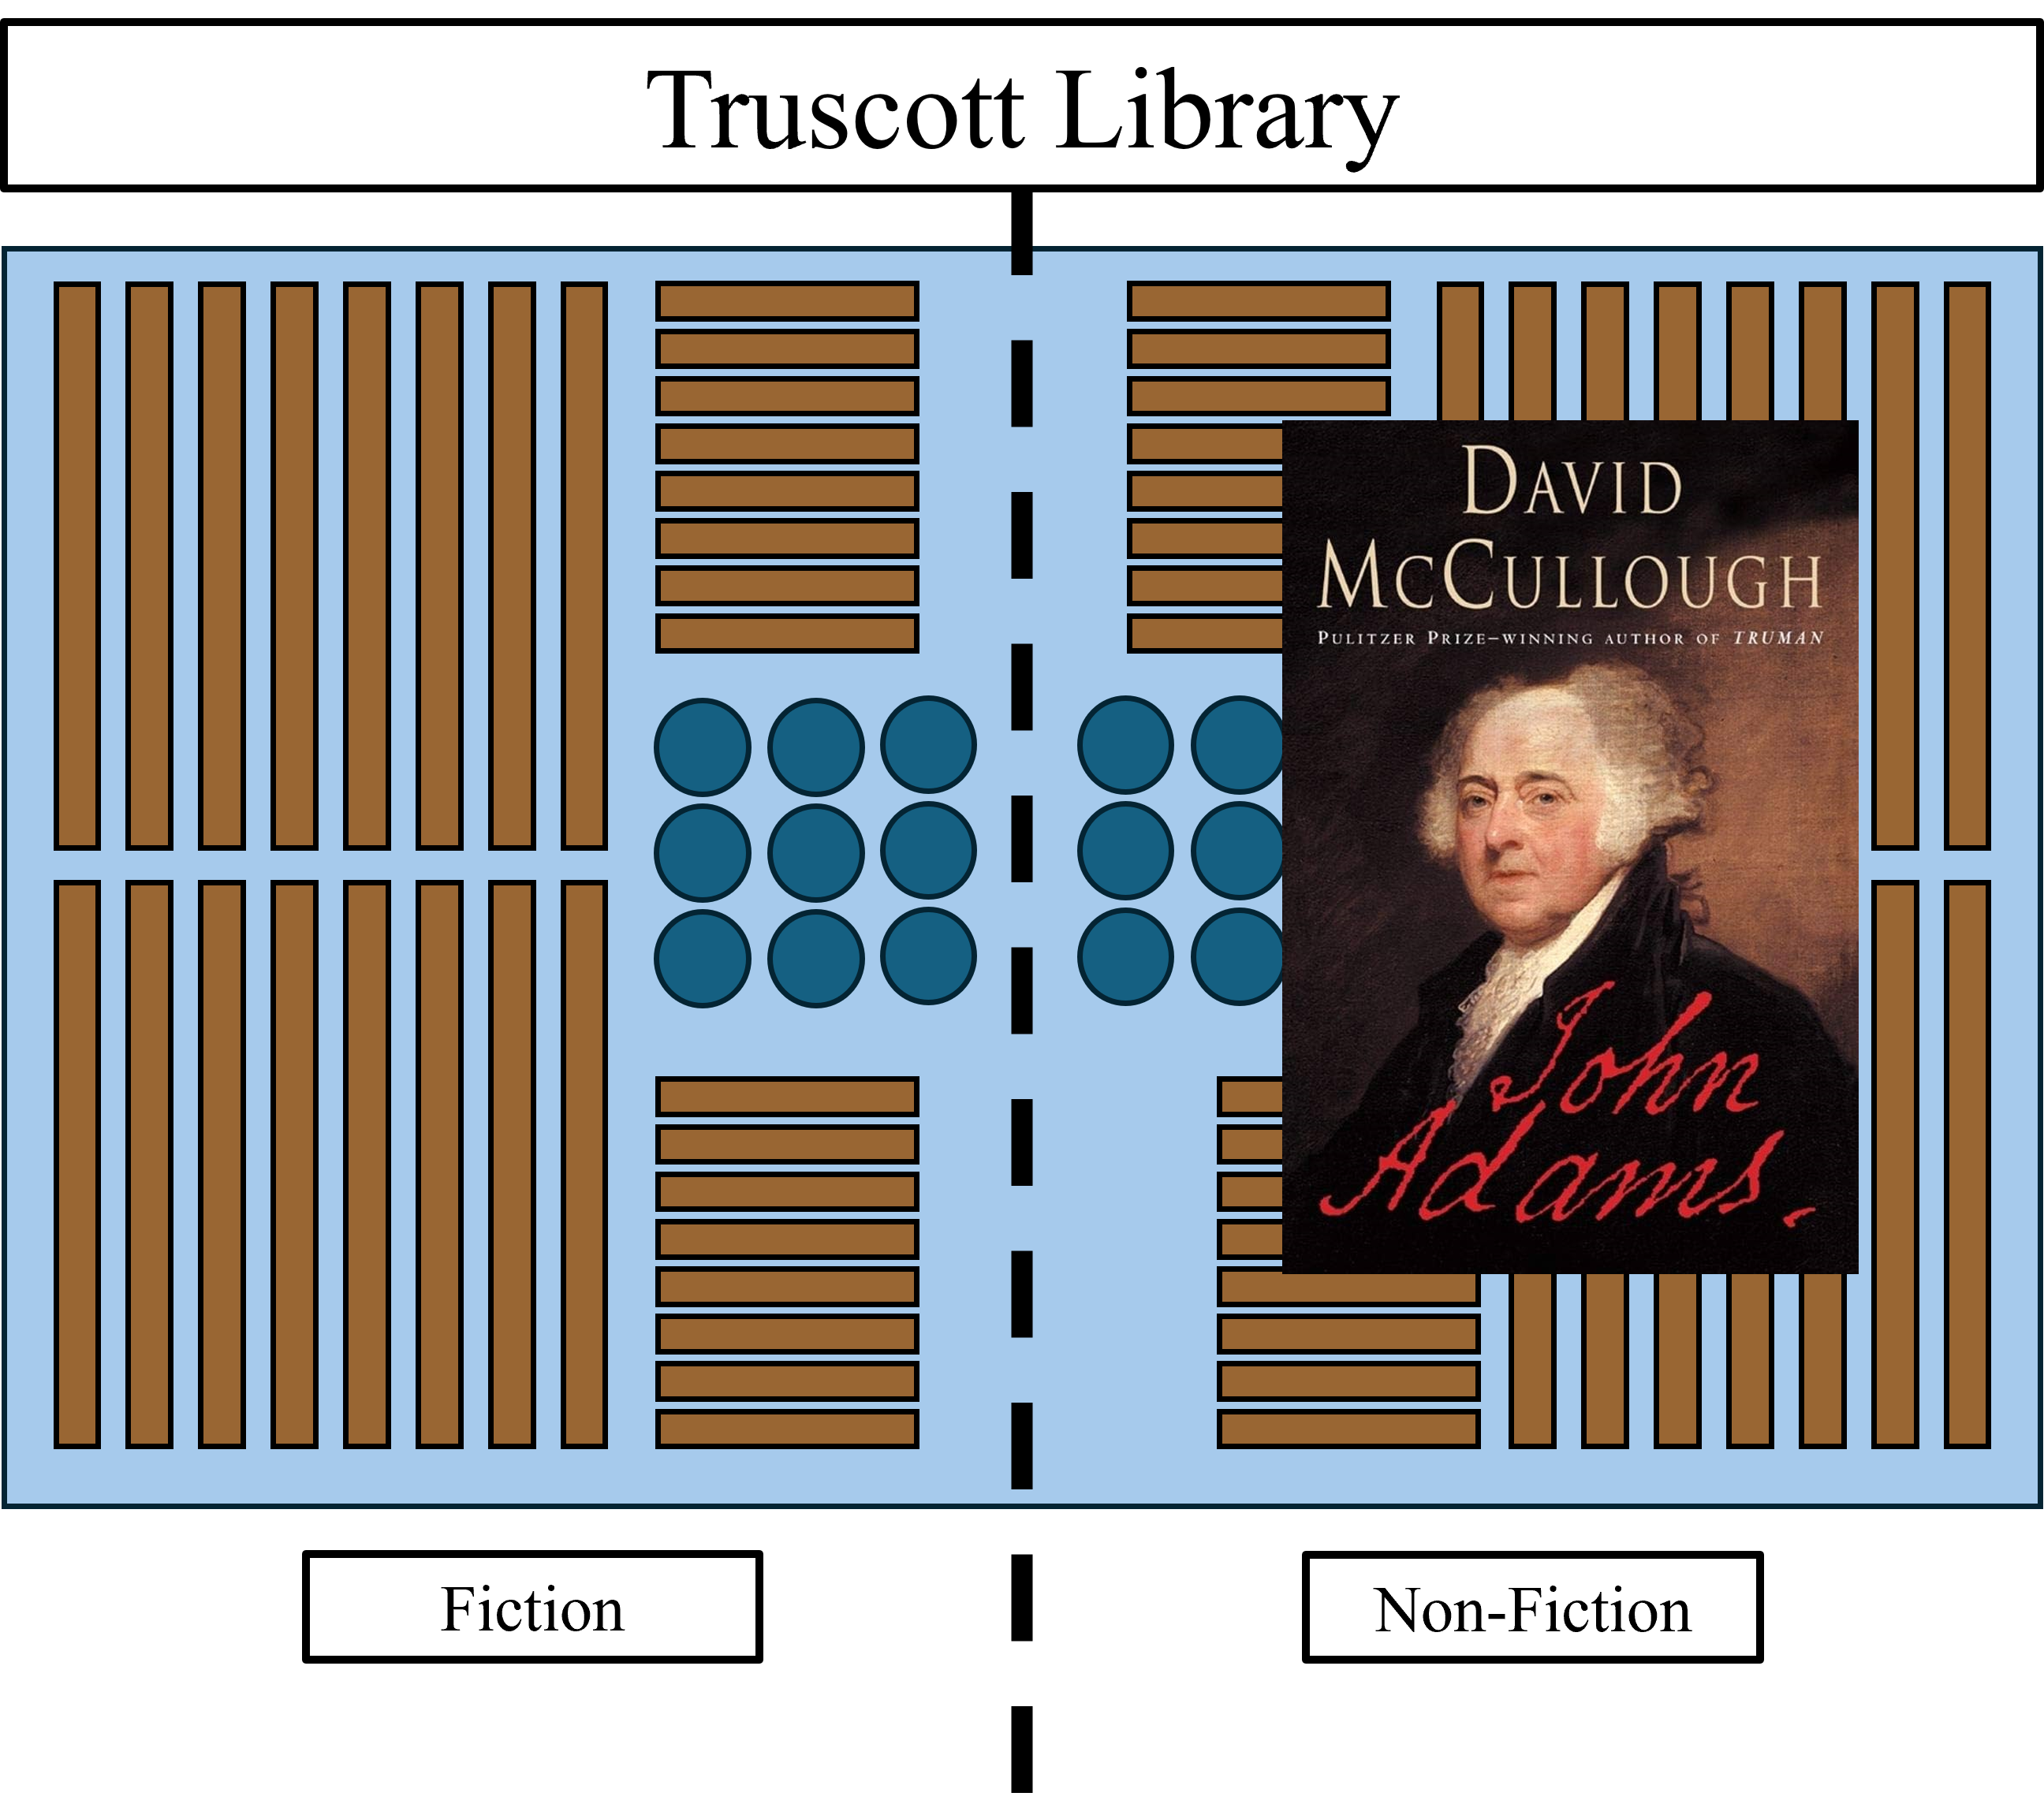
\includegraphics[width=0.55\textwidth]{../supplemental_materials/library_4_C.1.png}
\end{figure}
\end{frame}

\begin{frame}{Library Analogy (Cont.)}
\phantomsection\label{library-analogy-cont.-9}
\begin{figure}
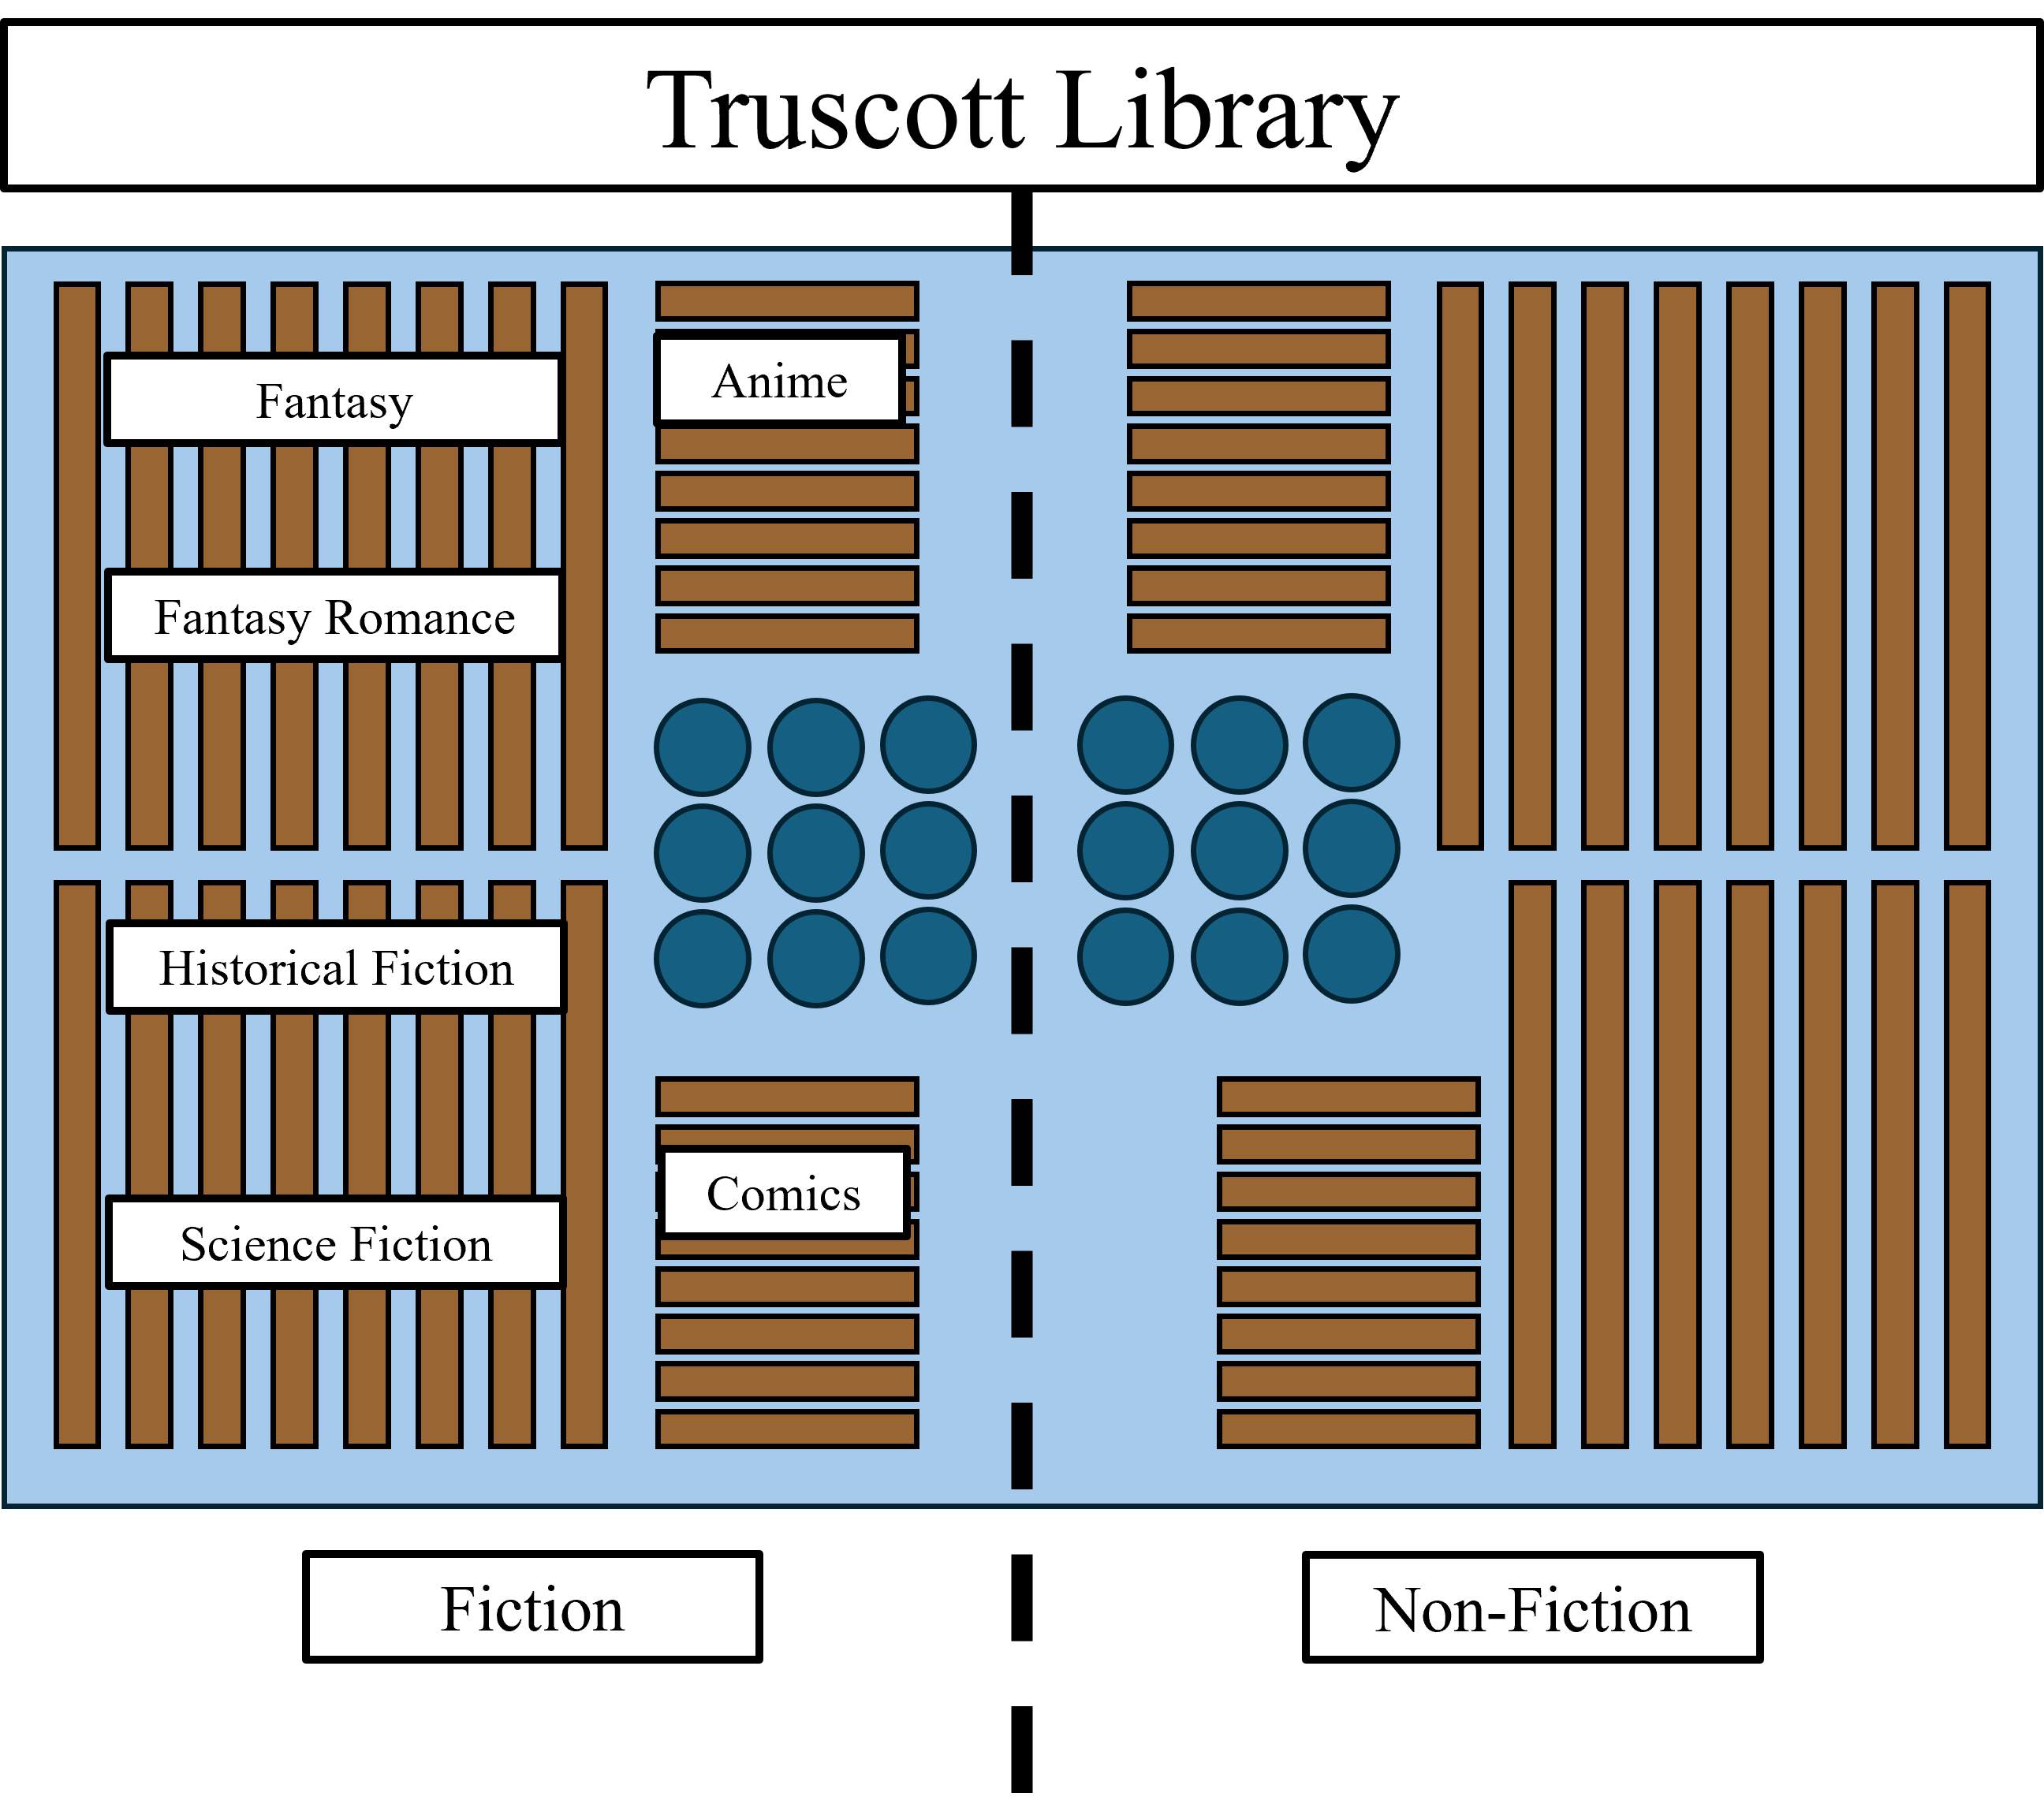
\includegraphics[width=0.55\textwidth]{../supplemental_materials/library_5.png}
\end{figure}
\end{frame}

\begin{frame}{Library Analogy (Cont.)}
\phantomsection\label{library-analogy-cont.-10}
\begin{figure}
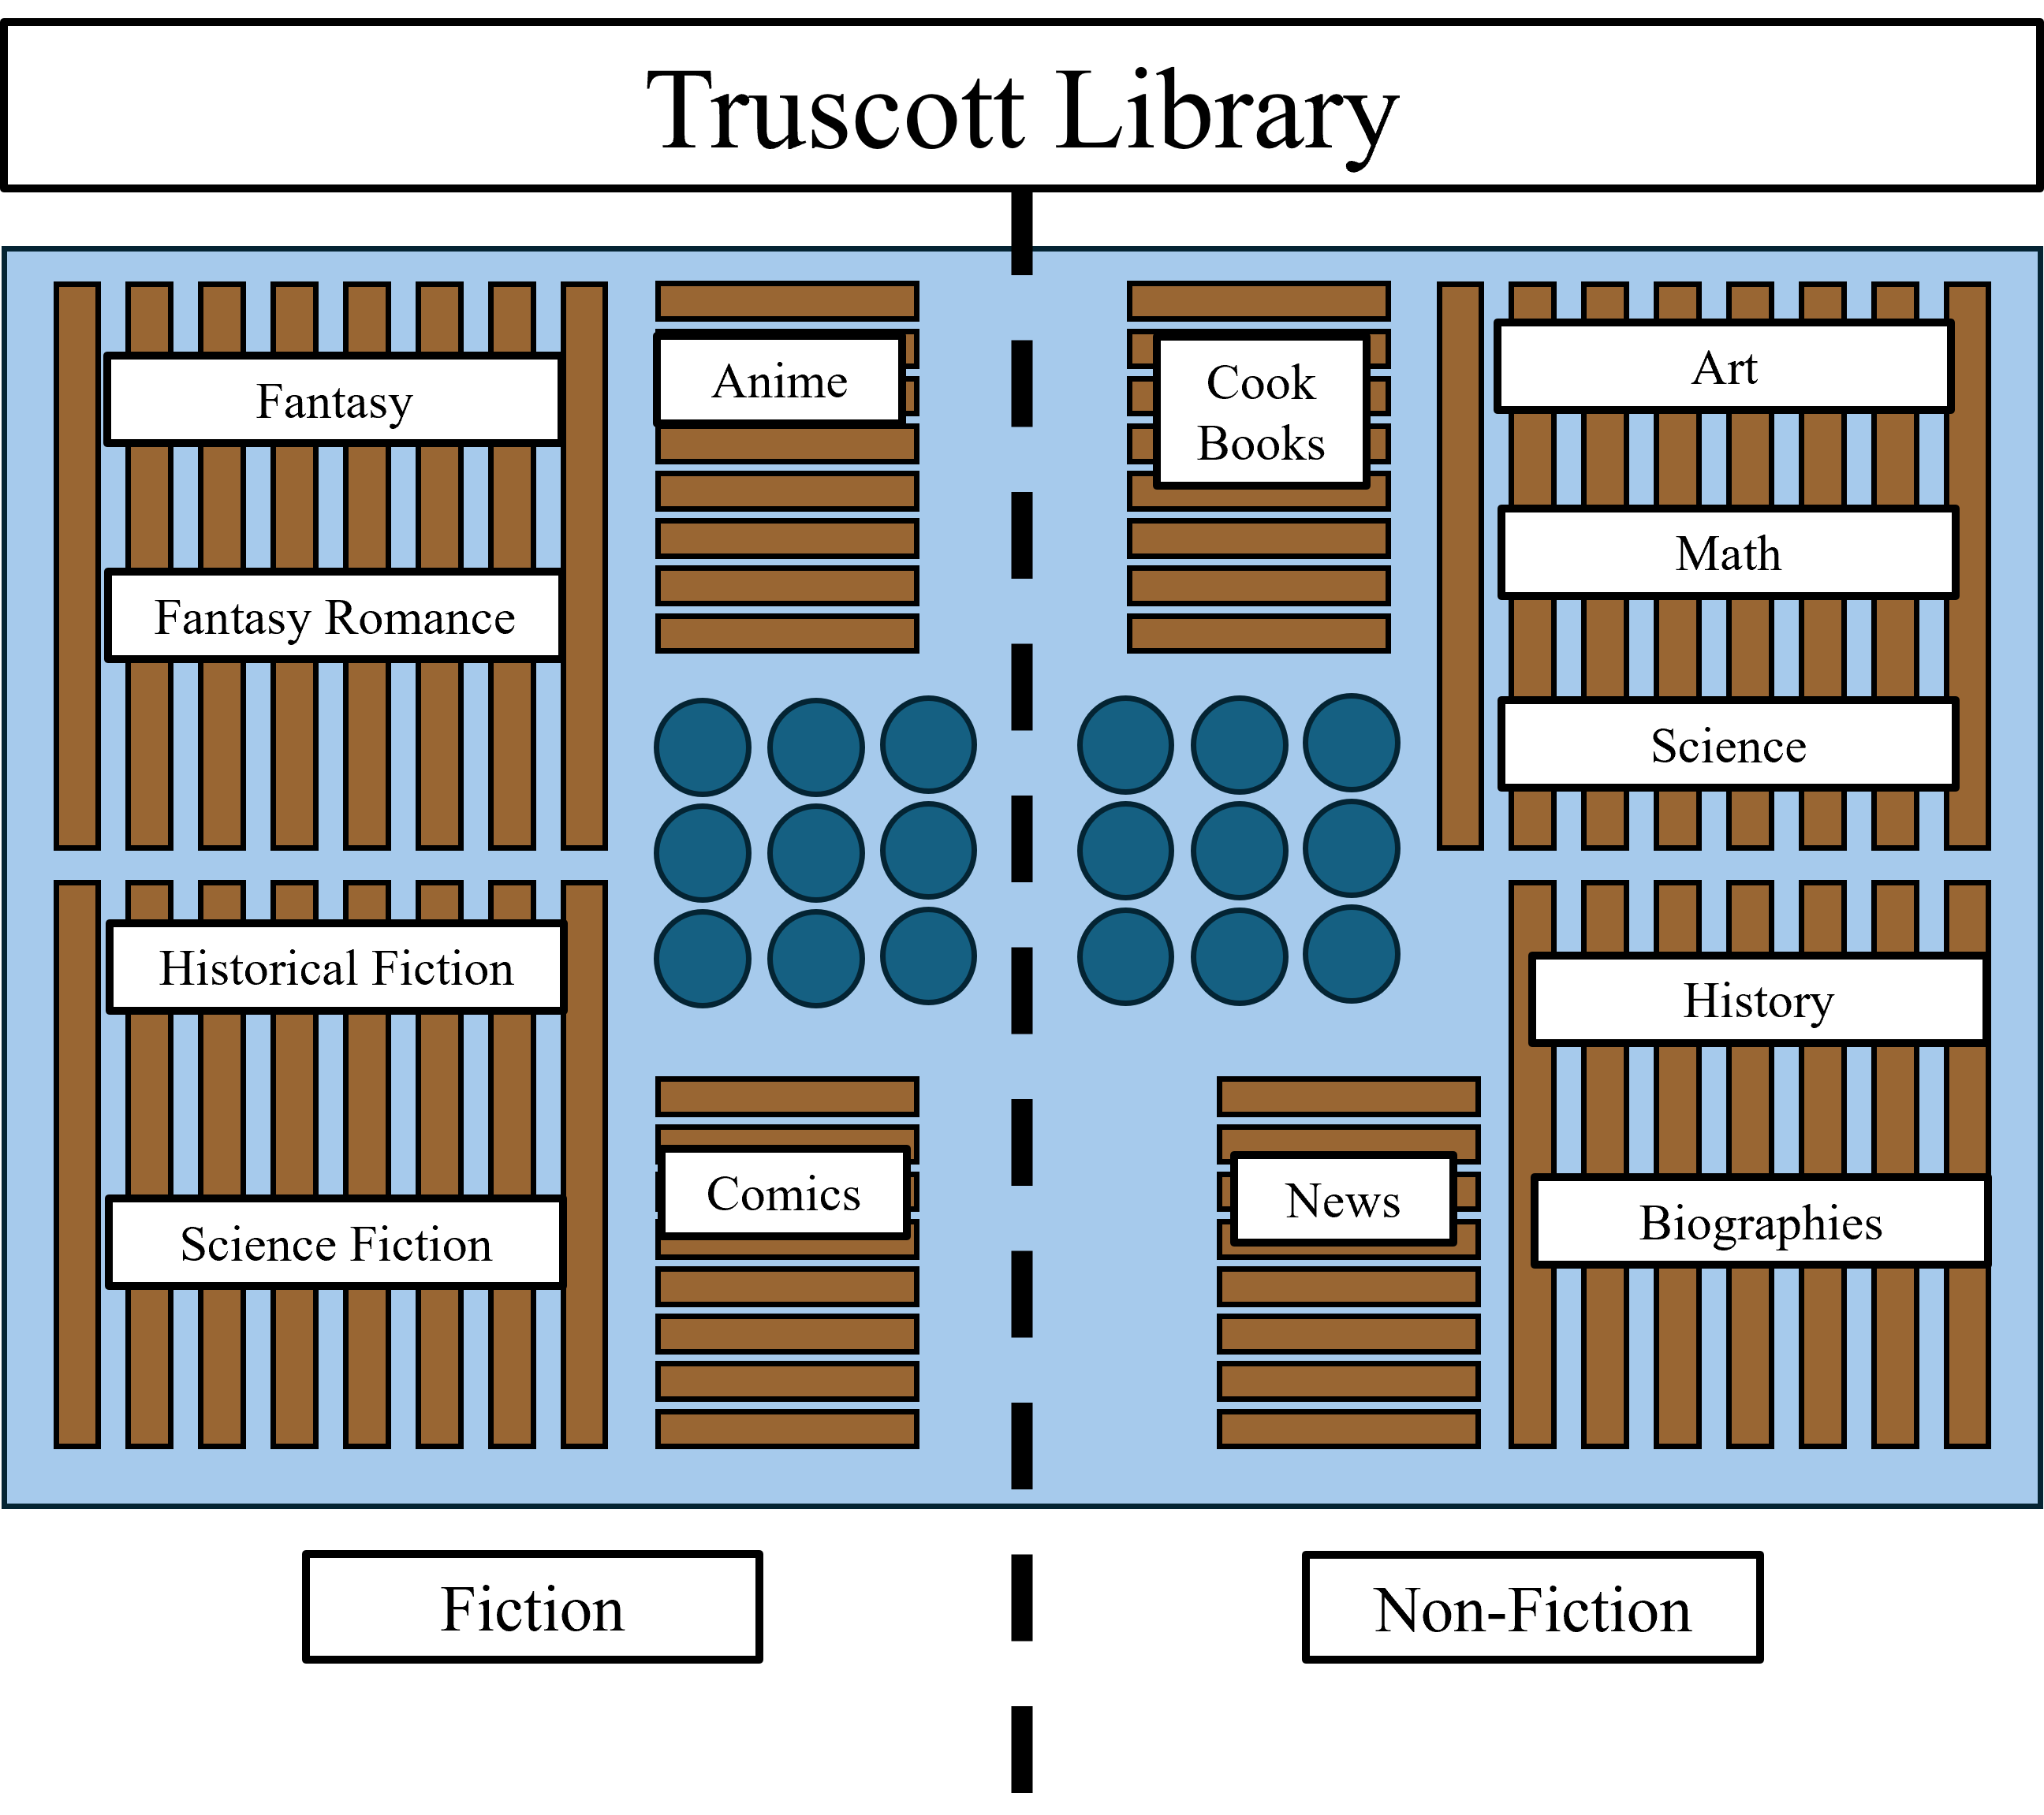
\includegraphics[width=0.55\textwidth]{../supplemental_materials/library_6.png}
\end{figure}
\end{frame}

\begin{frame}{Library Analogy (Cont.)}
\phantomsection\label{library-analogy-cont.-11}
\begin{figure}
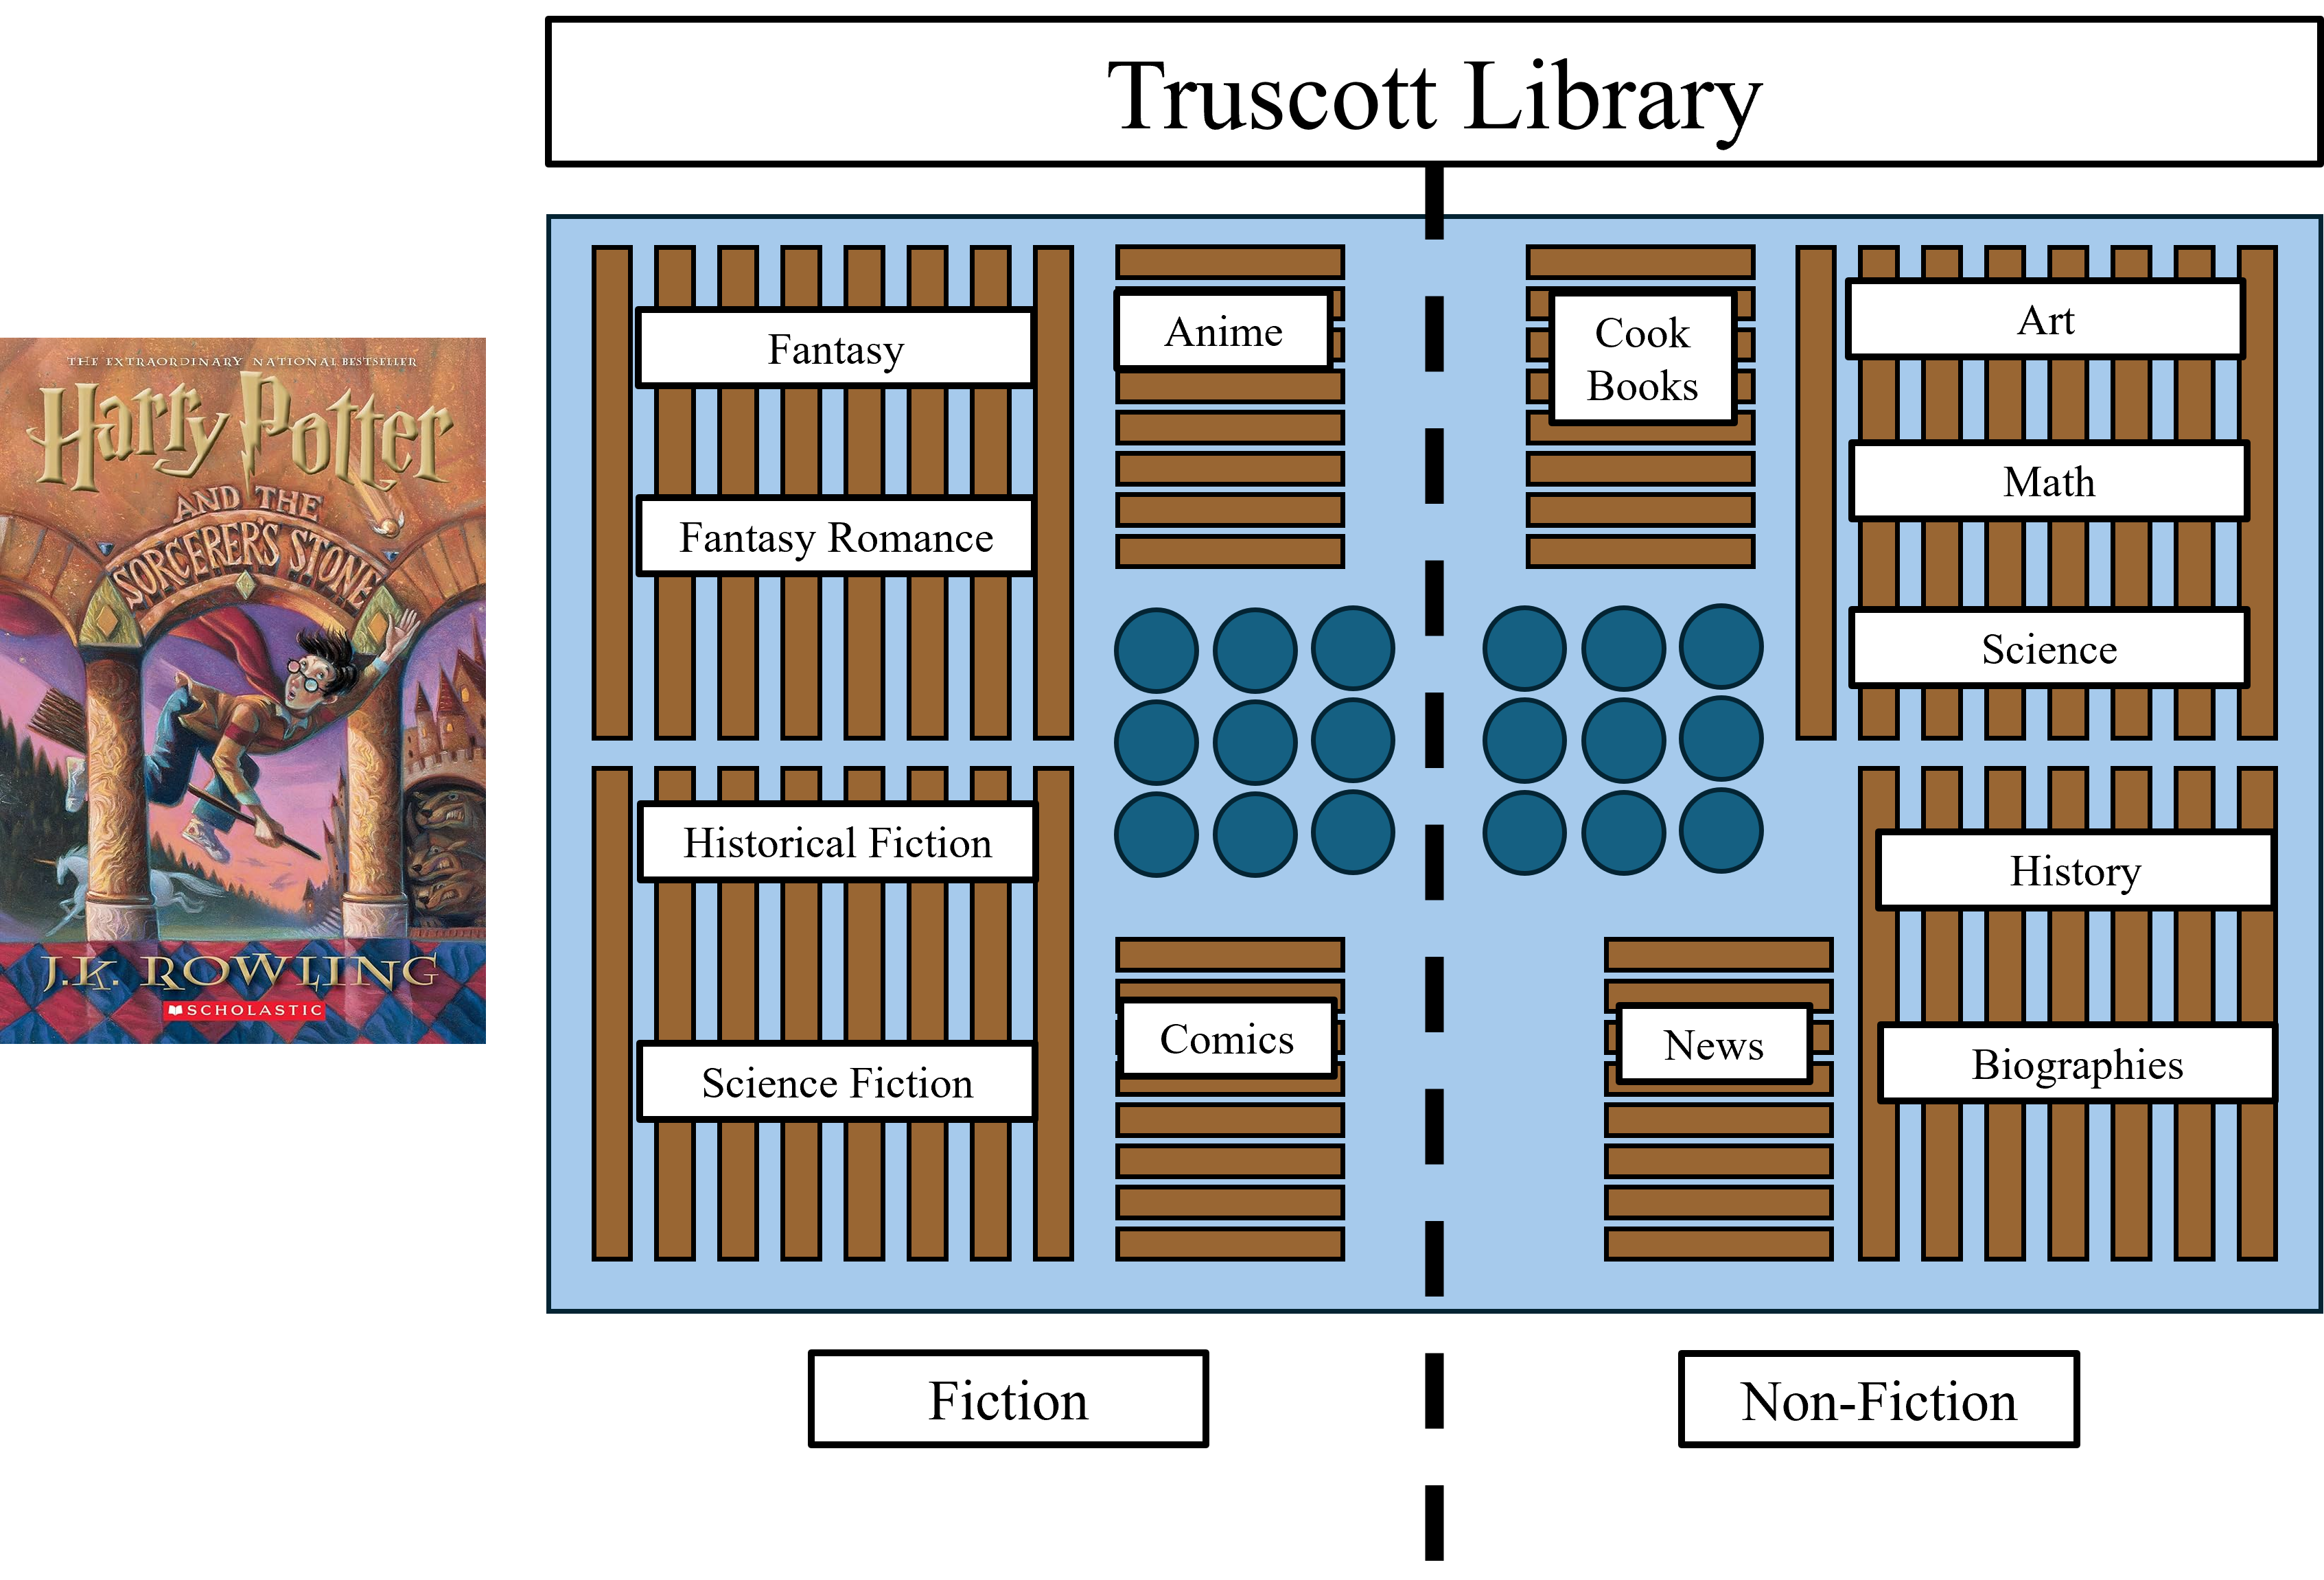
\includegraphics[width=0.55\textwidth]{../supplemental_materials/library_7.png}
\end{figure}
\end{frame}

\begin{frame}{Library Analogy (Cont.)}
\phantomsection\label{library-analogy-cont.-12}
\begin{figure}
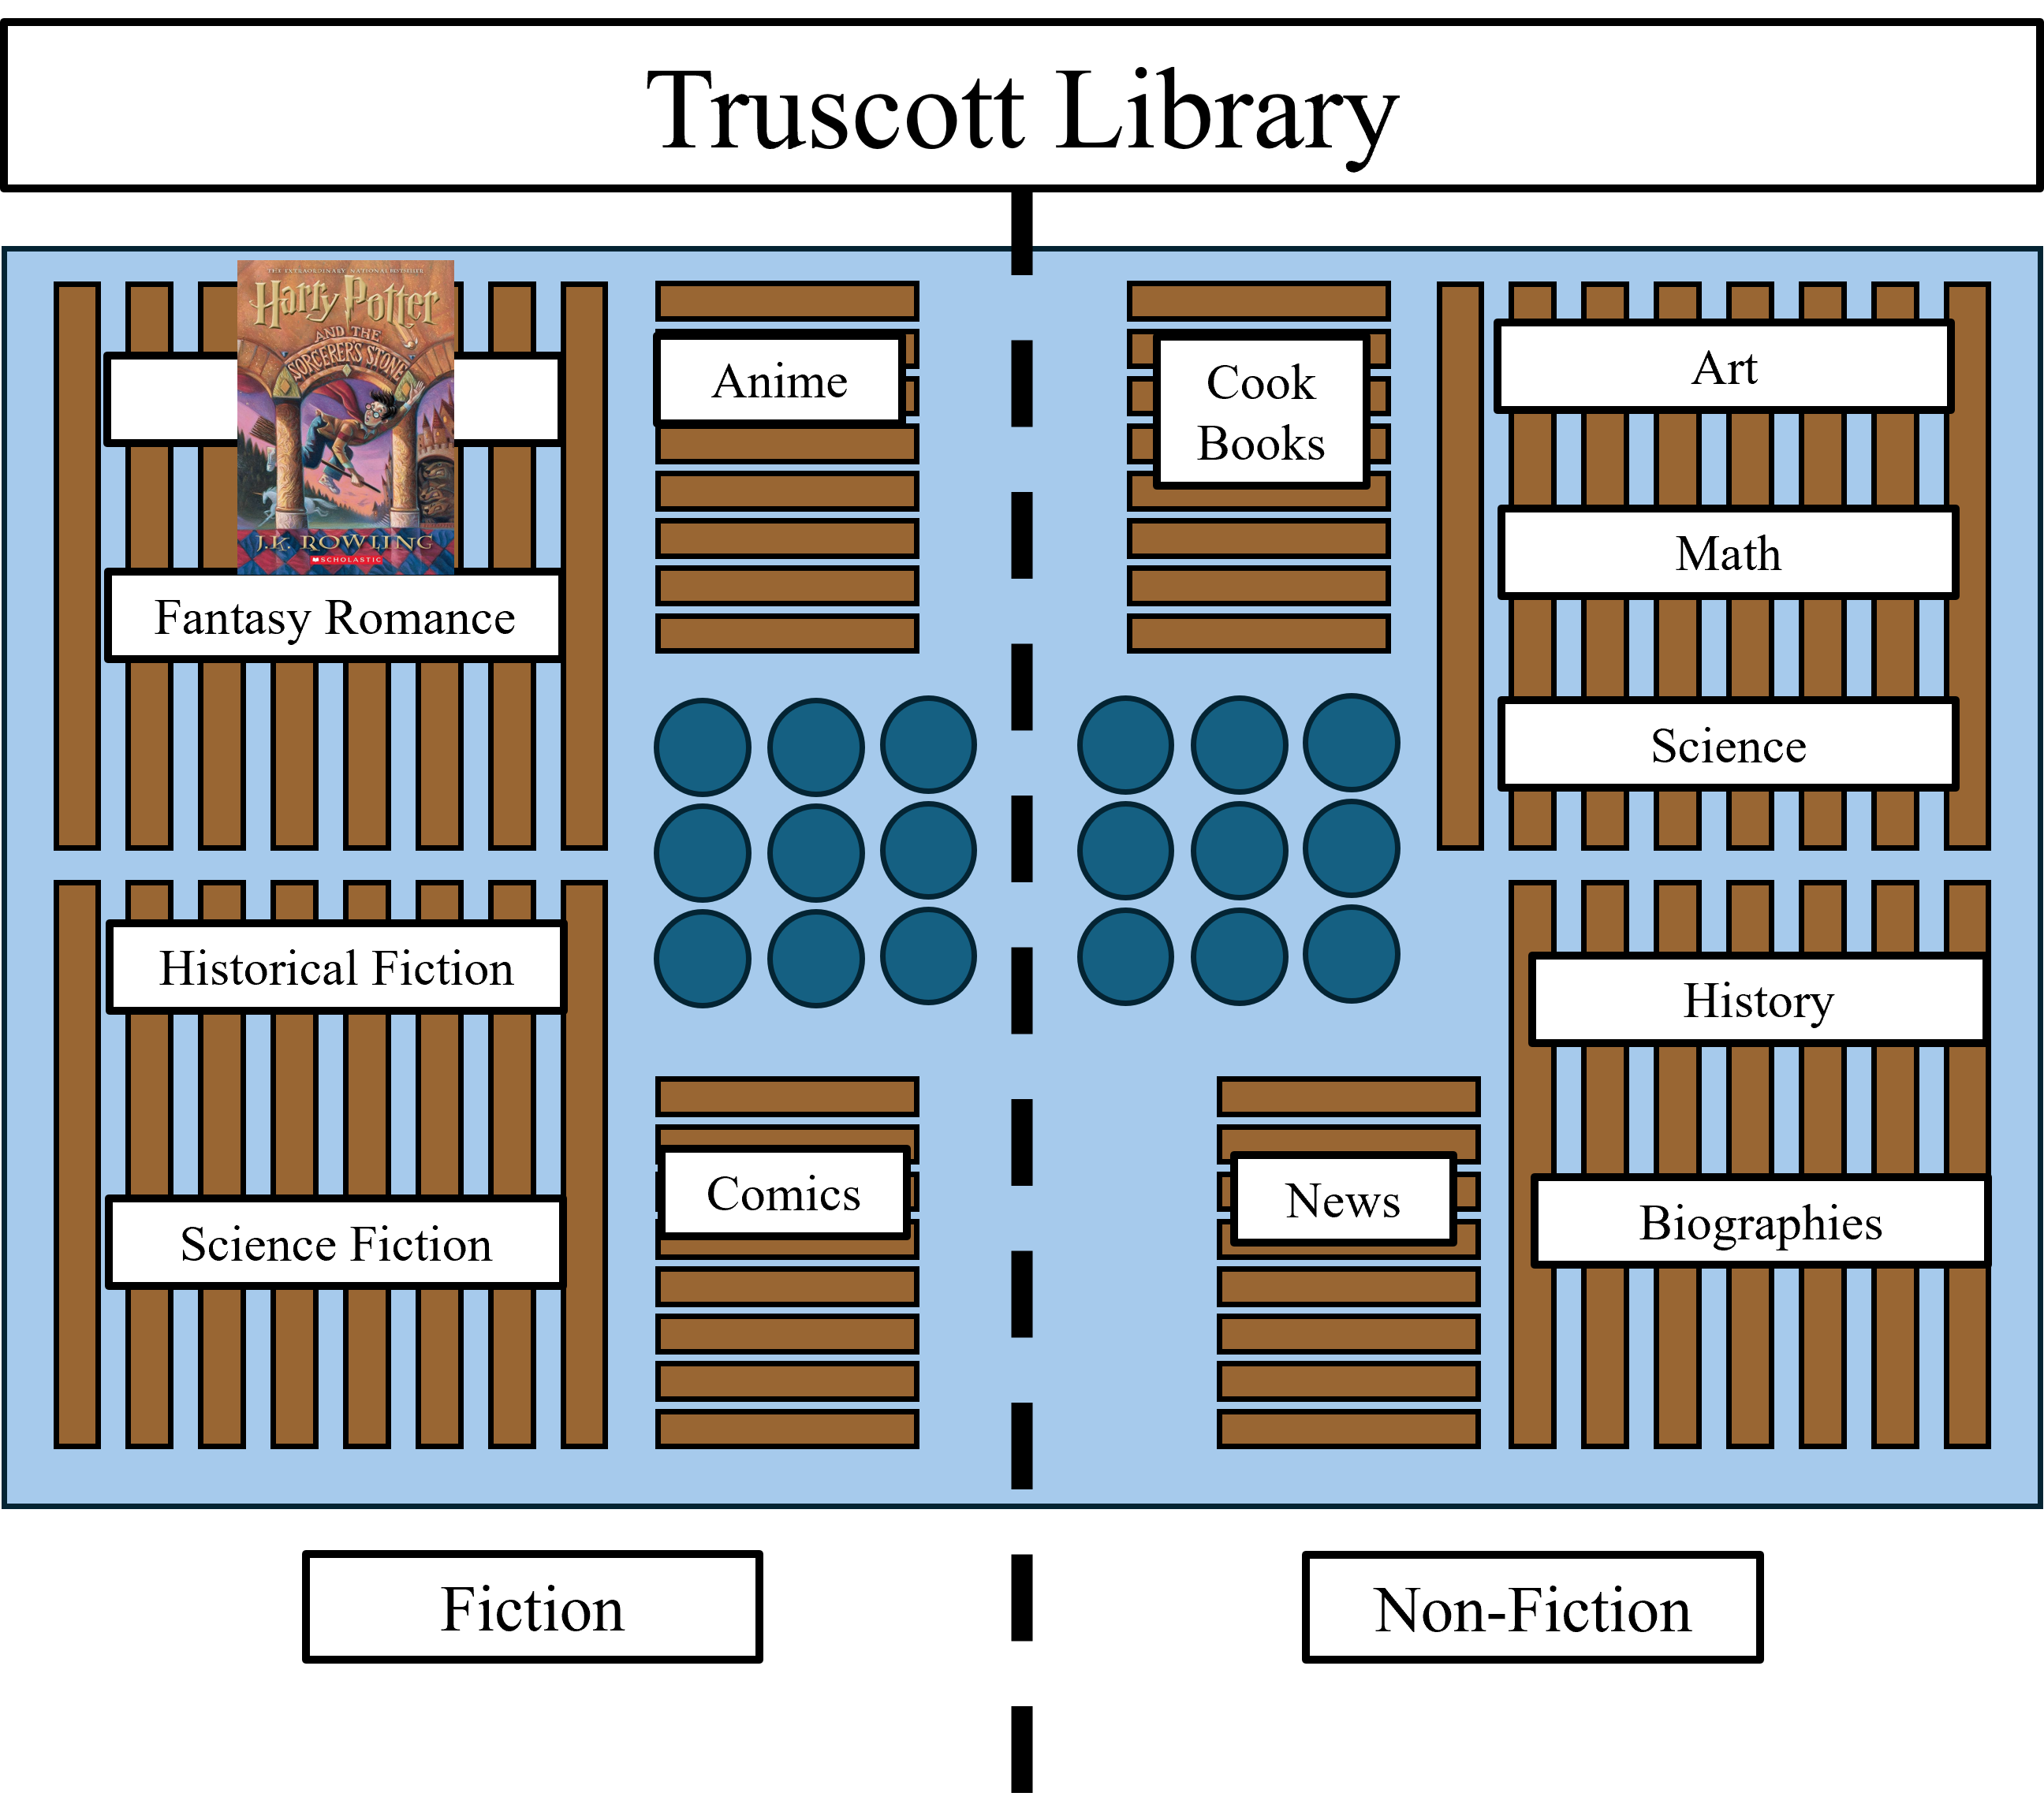
\includegraphics[width=0.55\textwidth]{../supplemental_materials/library_8.png}
\end{figure}
\end{frame}

\begin{frame}{Library Analogy (Cont.)}
\phantomsection\label{library-analogy-cont.-13}
\begin{figure}
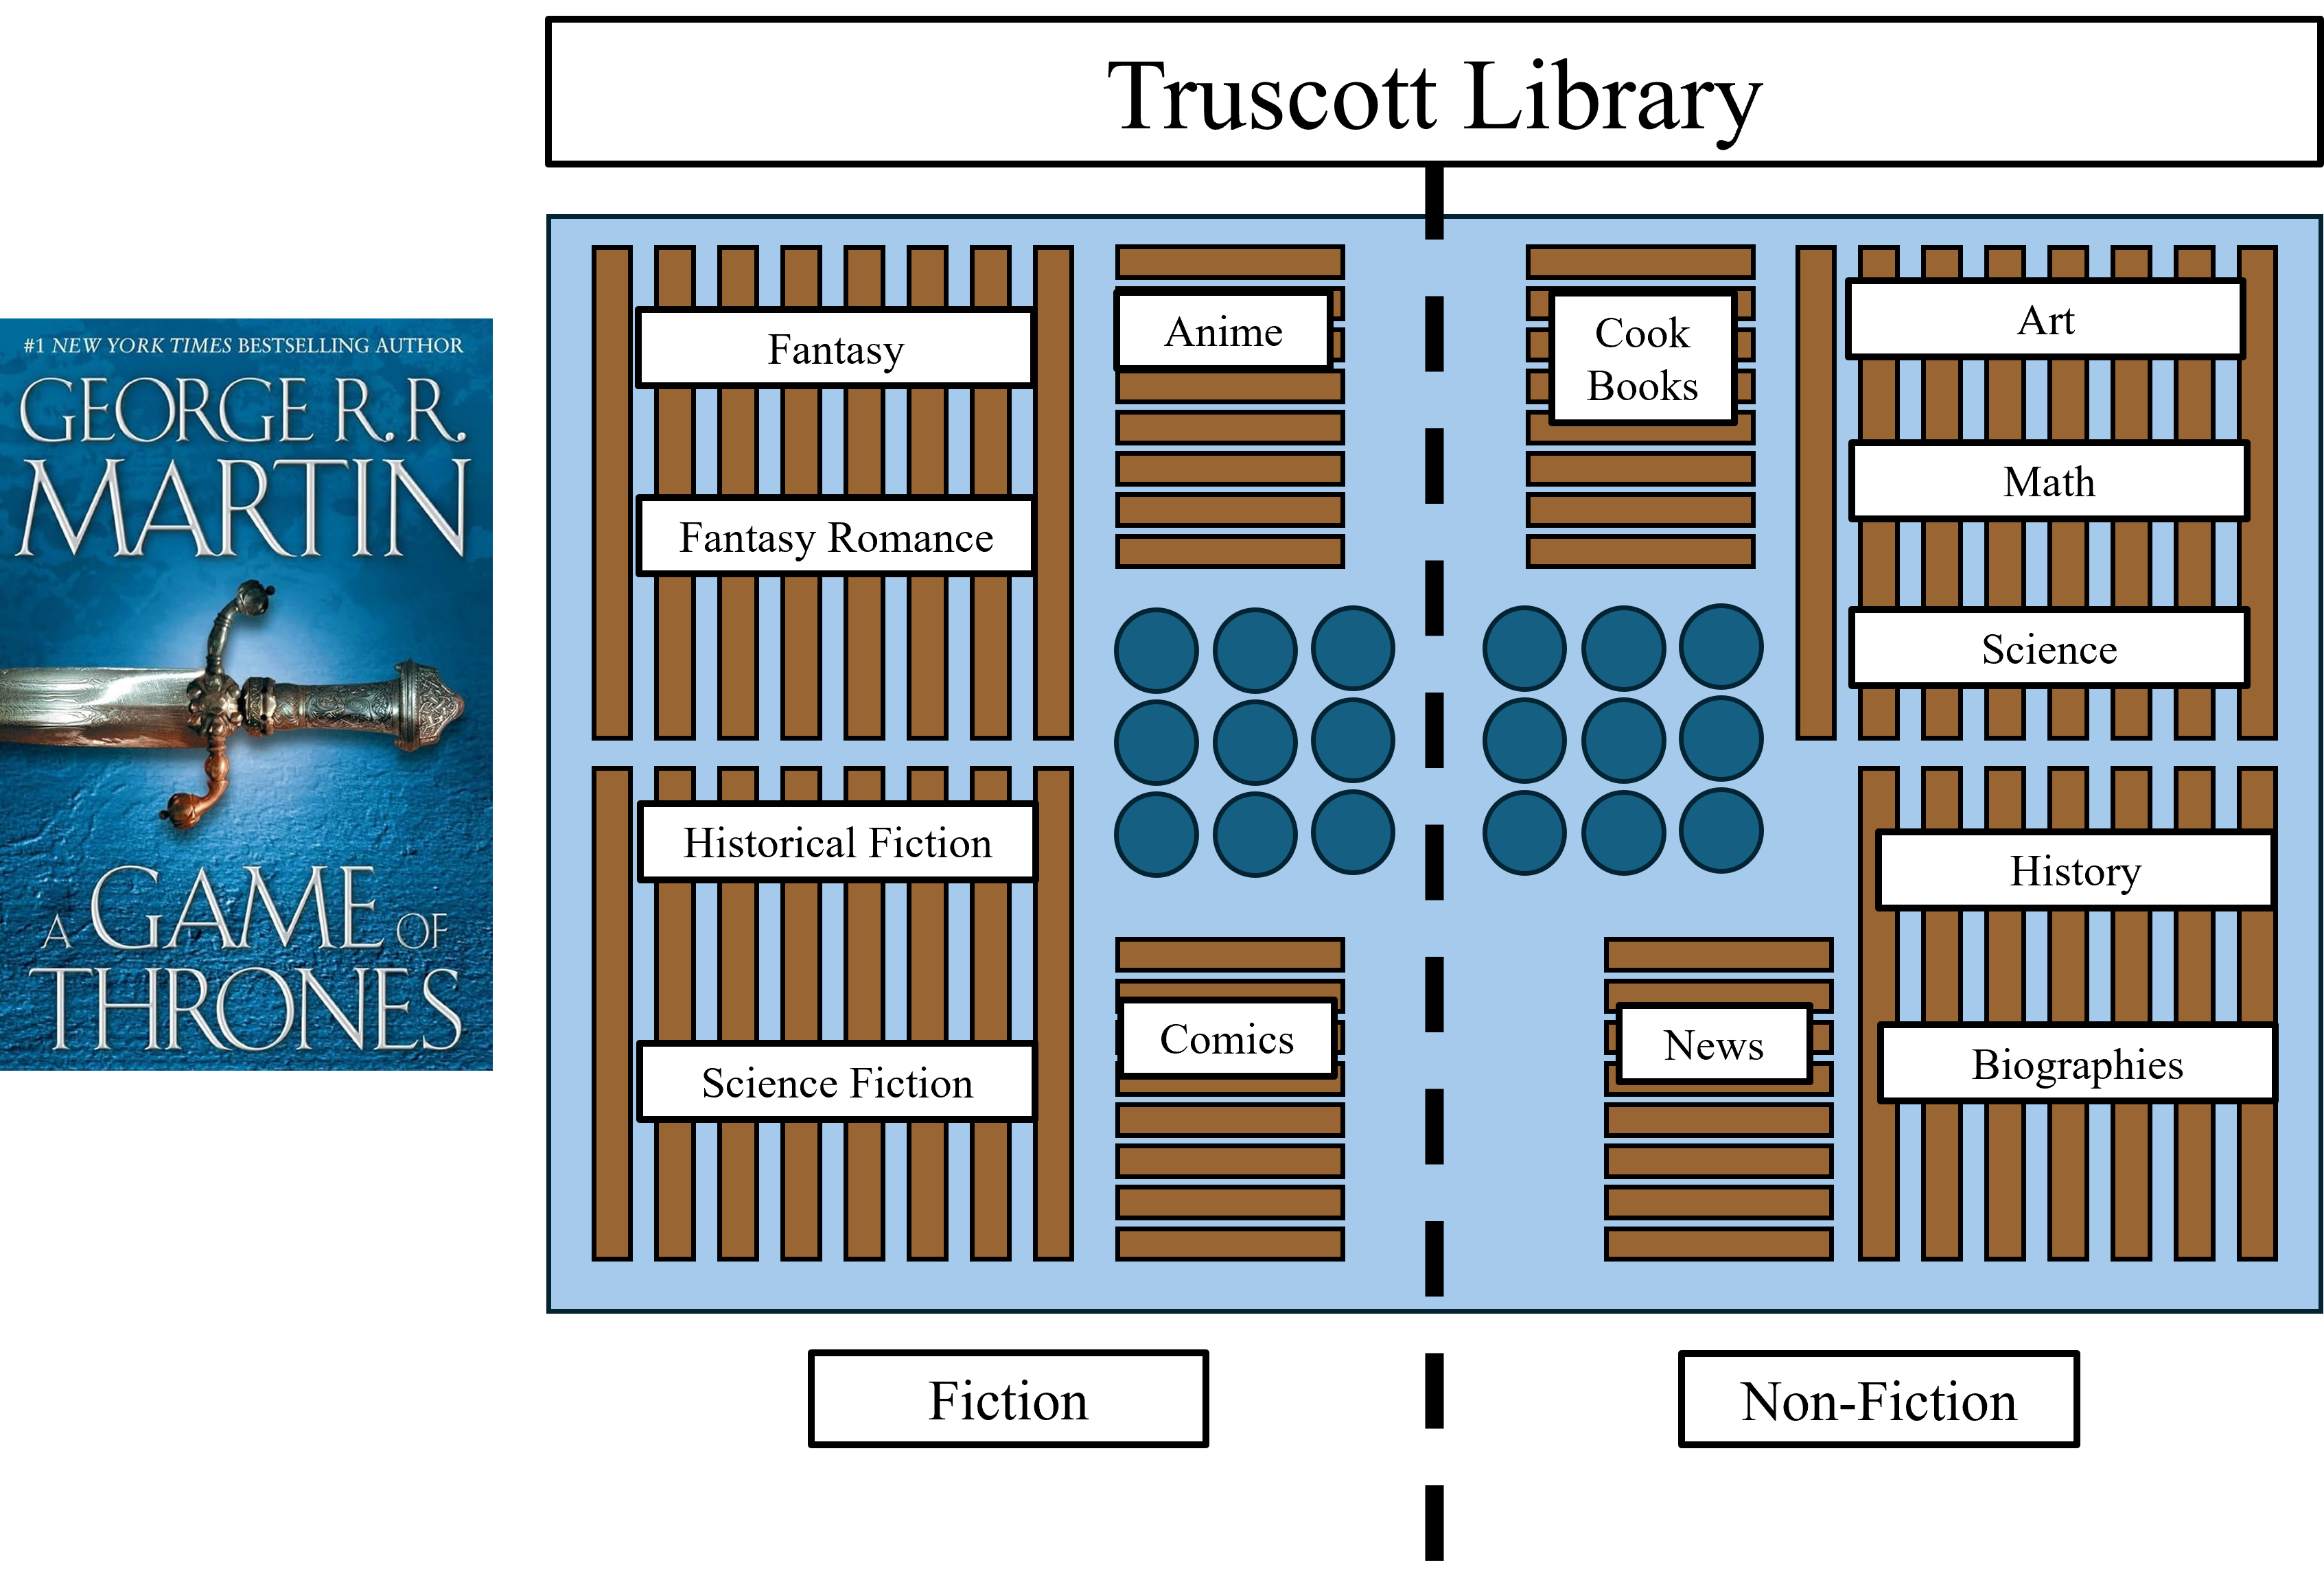
\includegraphics[width=0.55\textwidth]{../supplemental_materials/library_9.png}
\end{figure}
\end{frame}

\begin{frame}{Library Analogy (Cont.)}
\phantomsection\label{library-analogy-cont.-14}
\begin{figure}
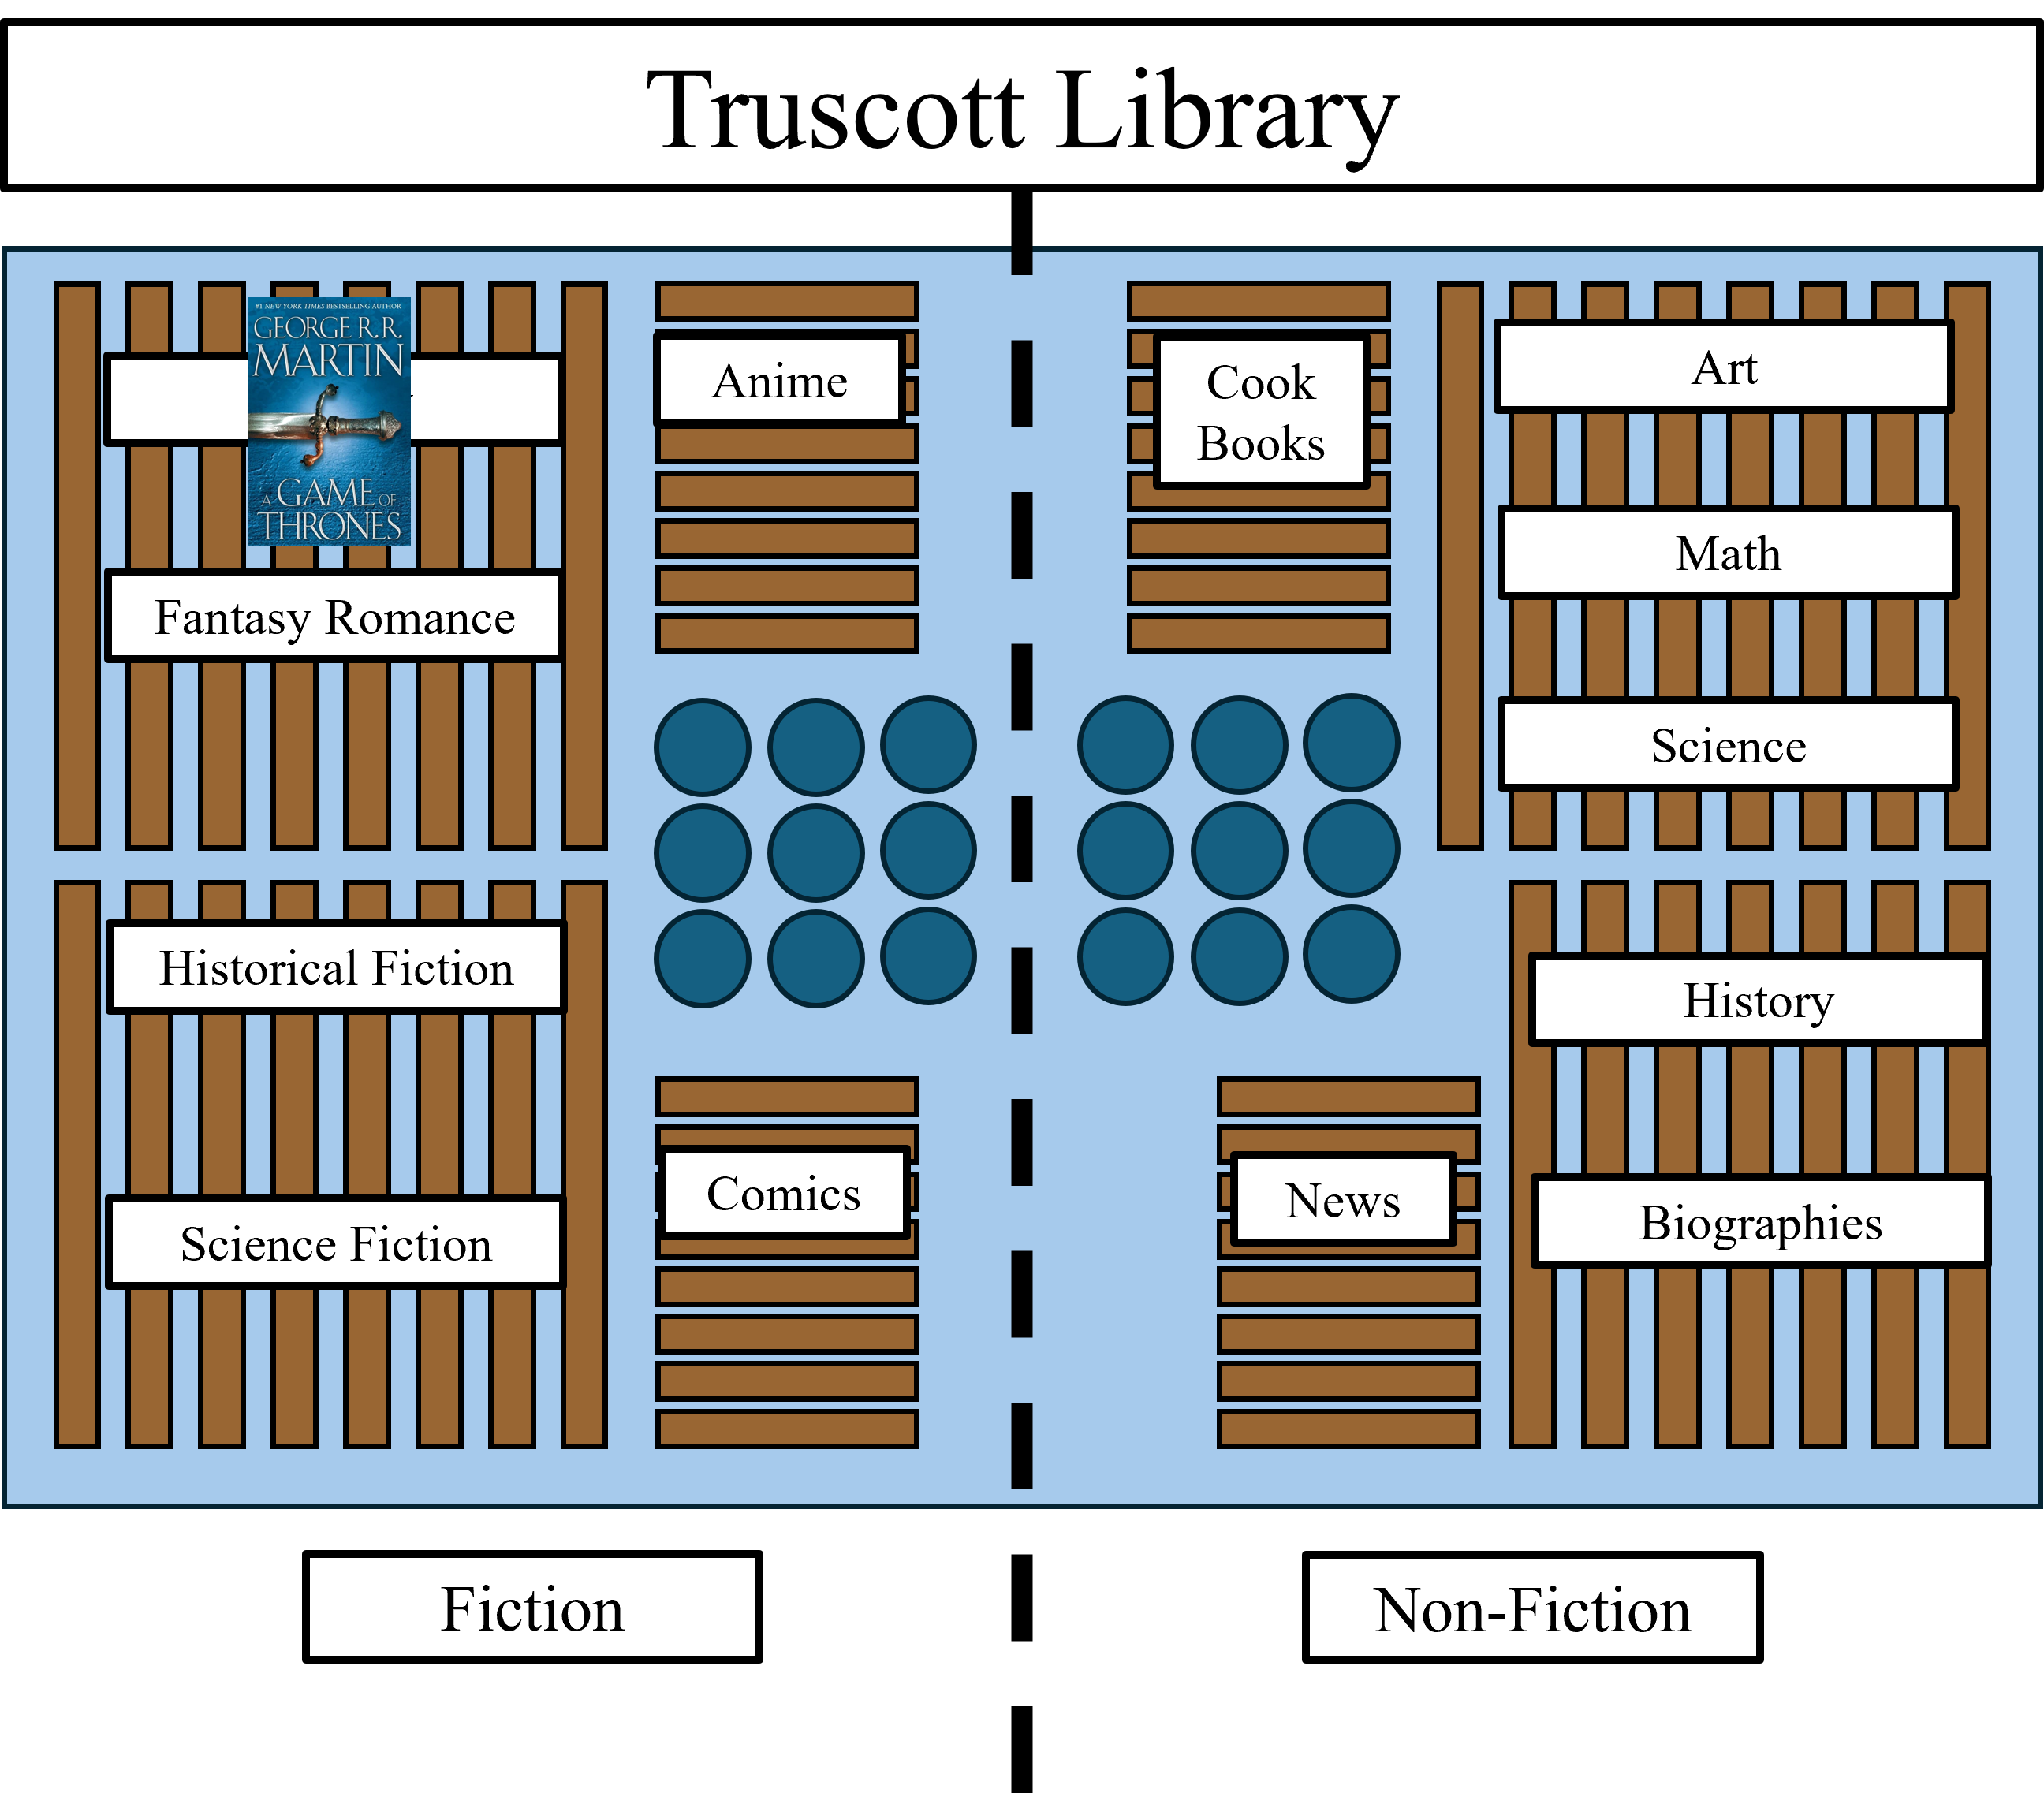
\includegraphics[width=0.55\textwidth]{../supplemental_materials/library_10.png}
\end{figure}
\end{frame}

\begin{frame}{Library Analogy (Cont.)}
\phantomsection\label{library-analogy-cont.-15}
\begin{figure}
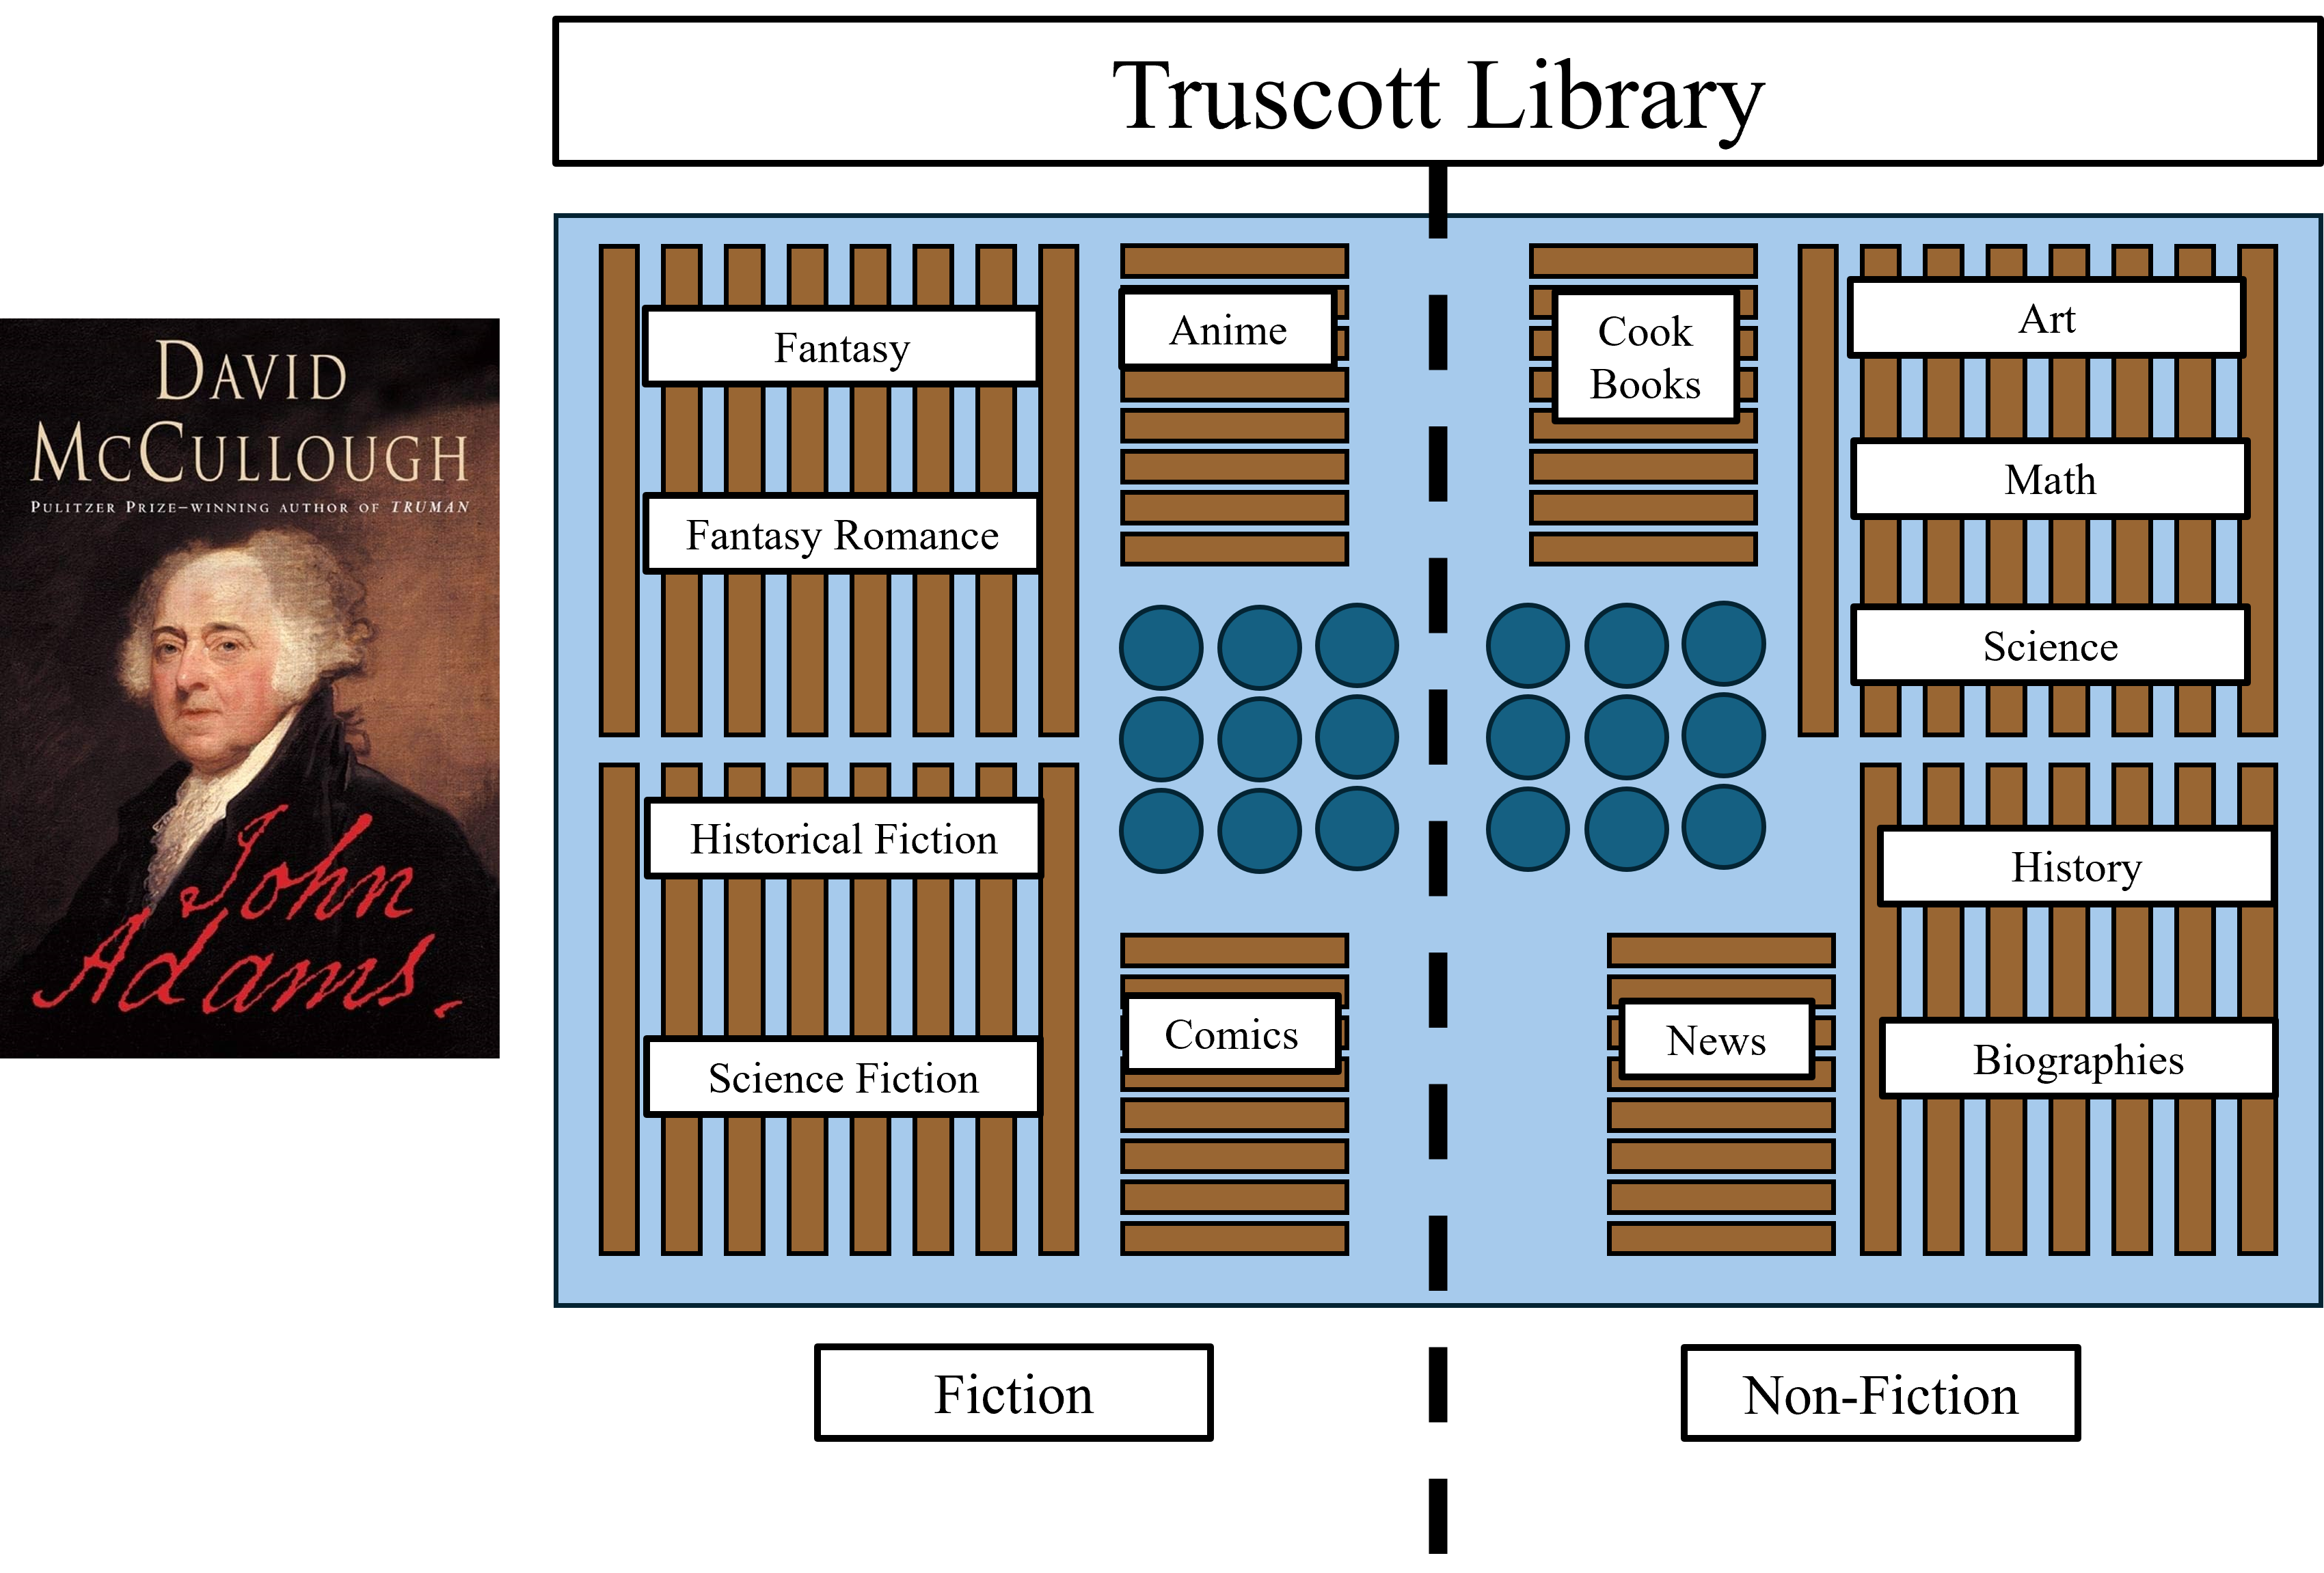
\includegraphics[width=0.55\textwidth]{../supplemental_materials/library_11.png}
\end{figure}
\end{frame}

\begin{frame}{Library Analogy (Cont.)}
\phantomsection\label{library-analogy-cont.-16}
\begin{figure}
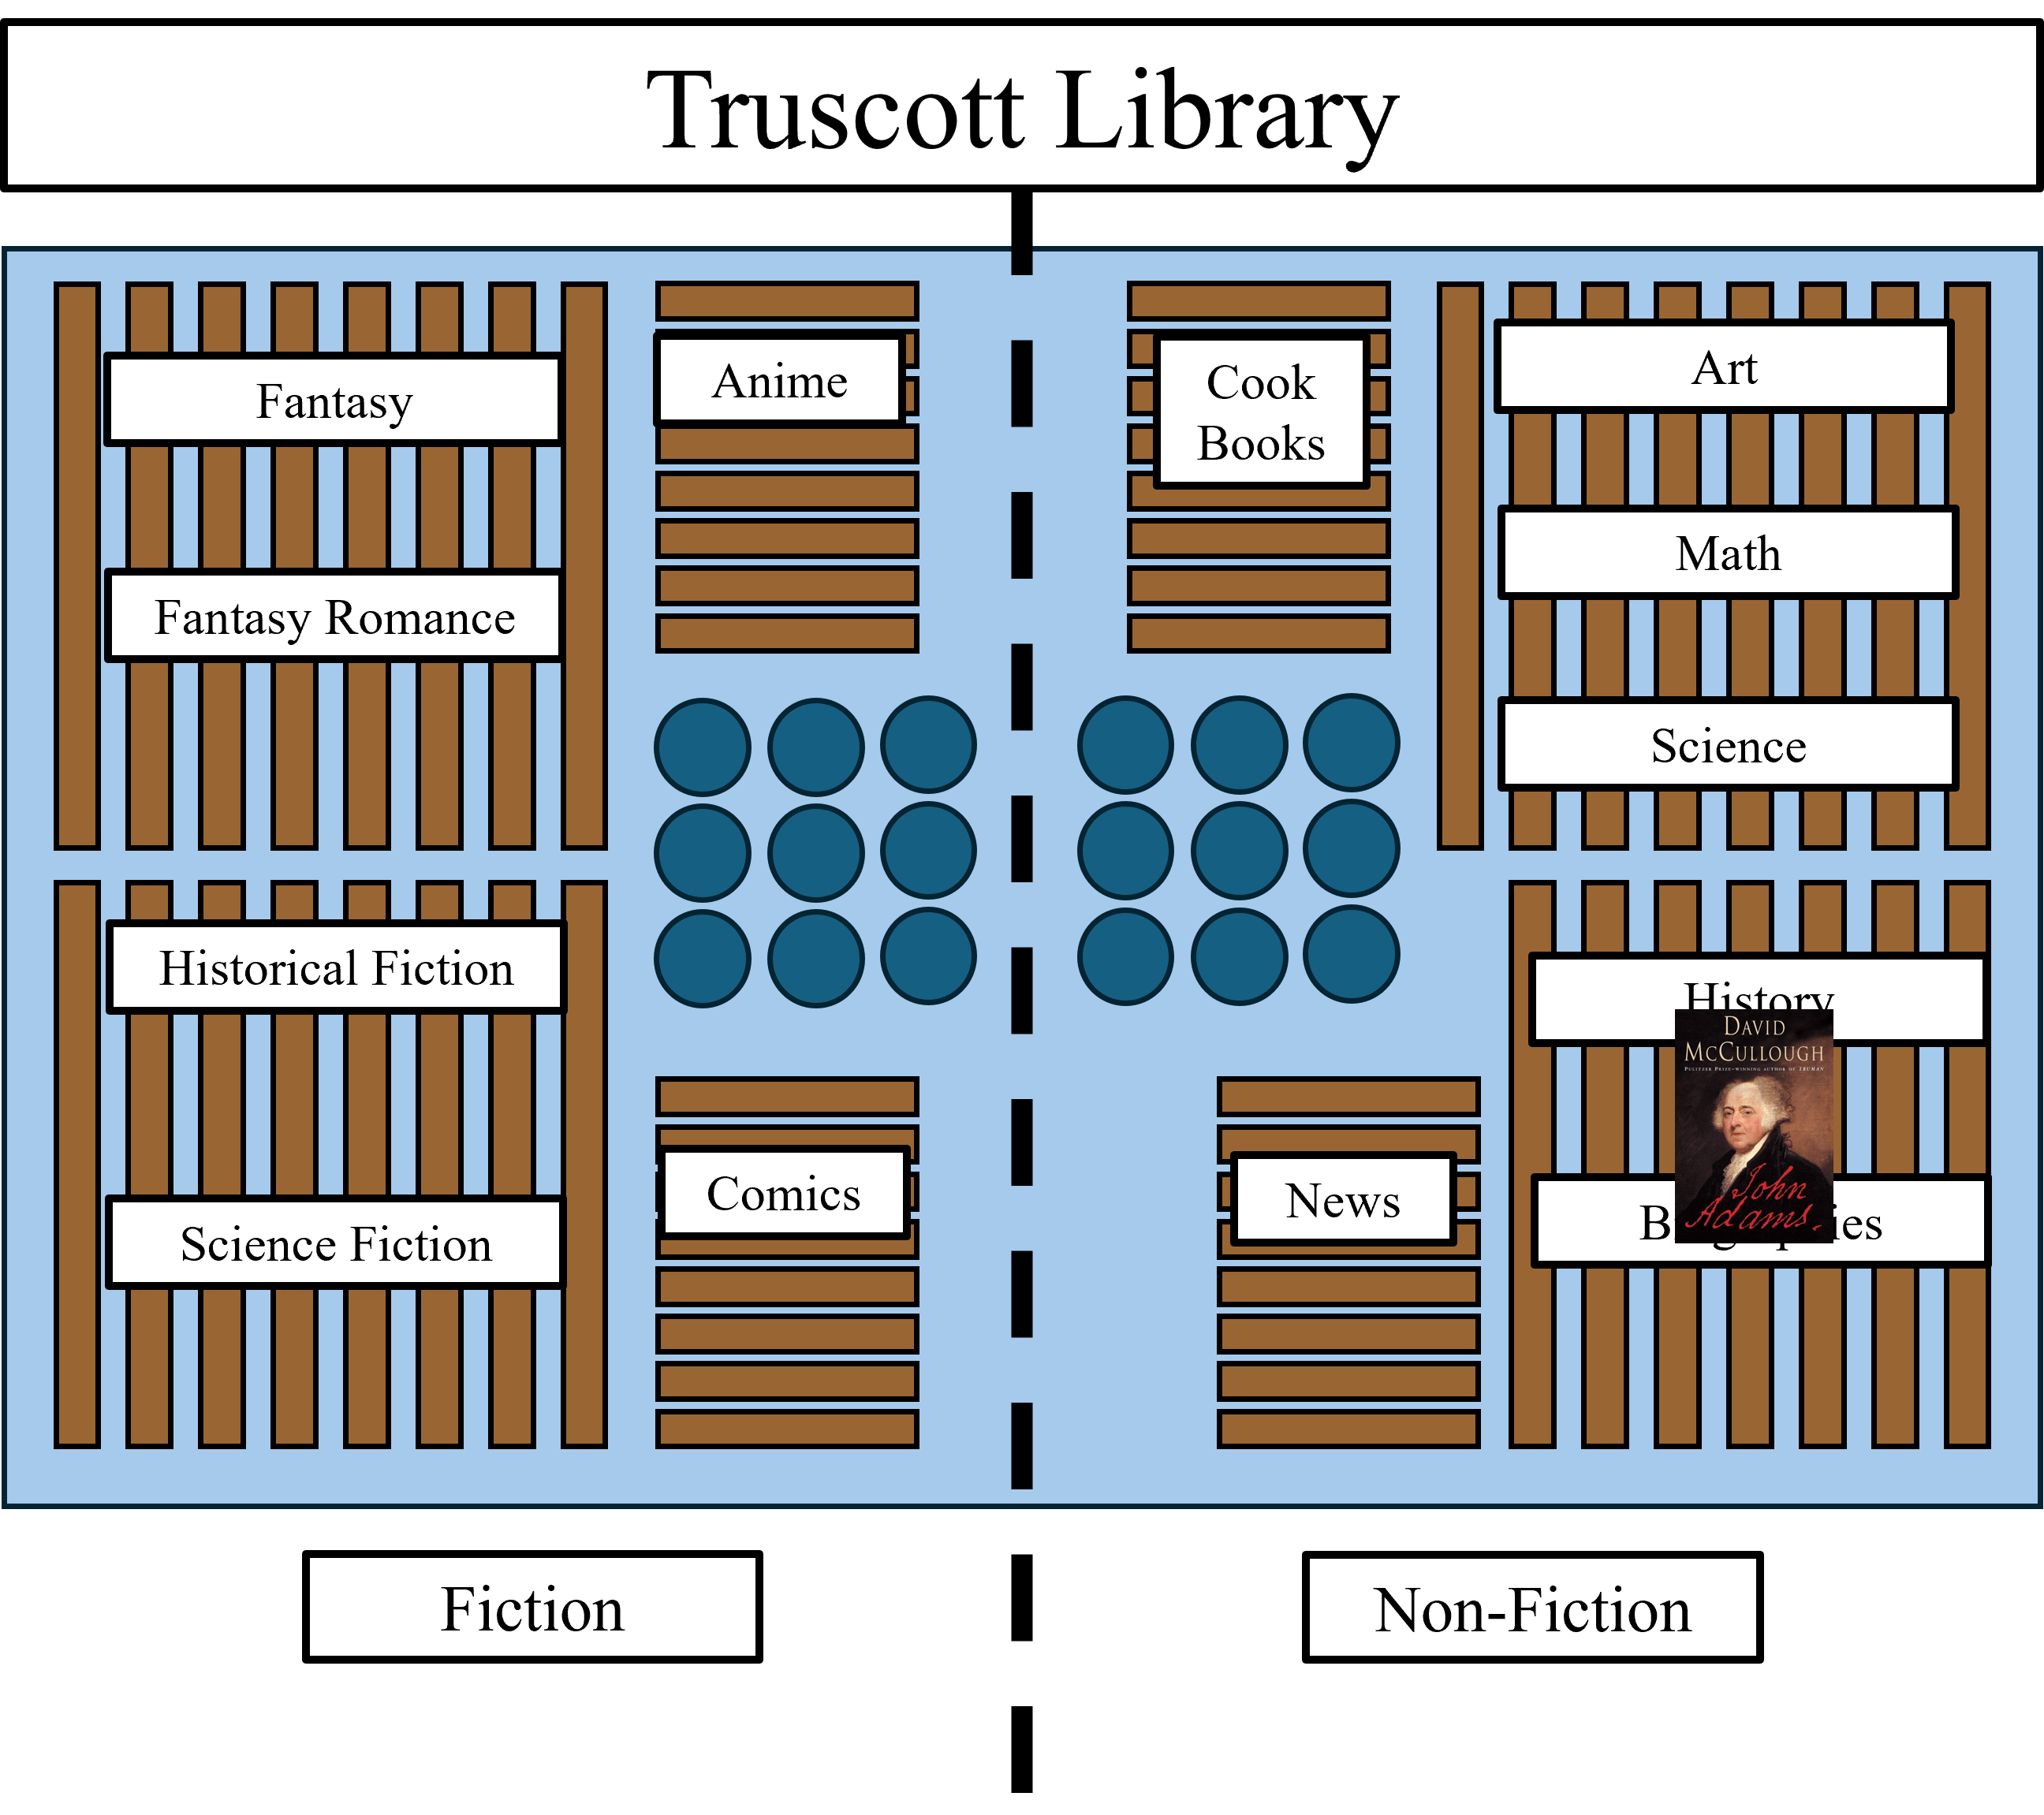
\includegraphics[width=0.55\textwidth]{../supplemental_materials/library_12.png}
\end{figure}
\end{frame}

\begin{frame}{Library Analogy (Cont.)}
\phantomsection\label{library-analogy-cont.-17}
\begin{figure}
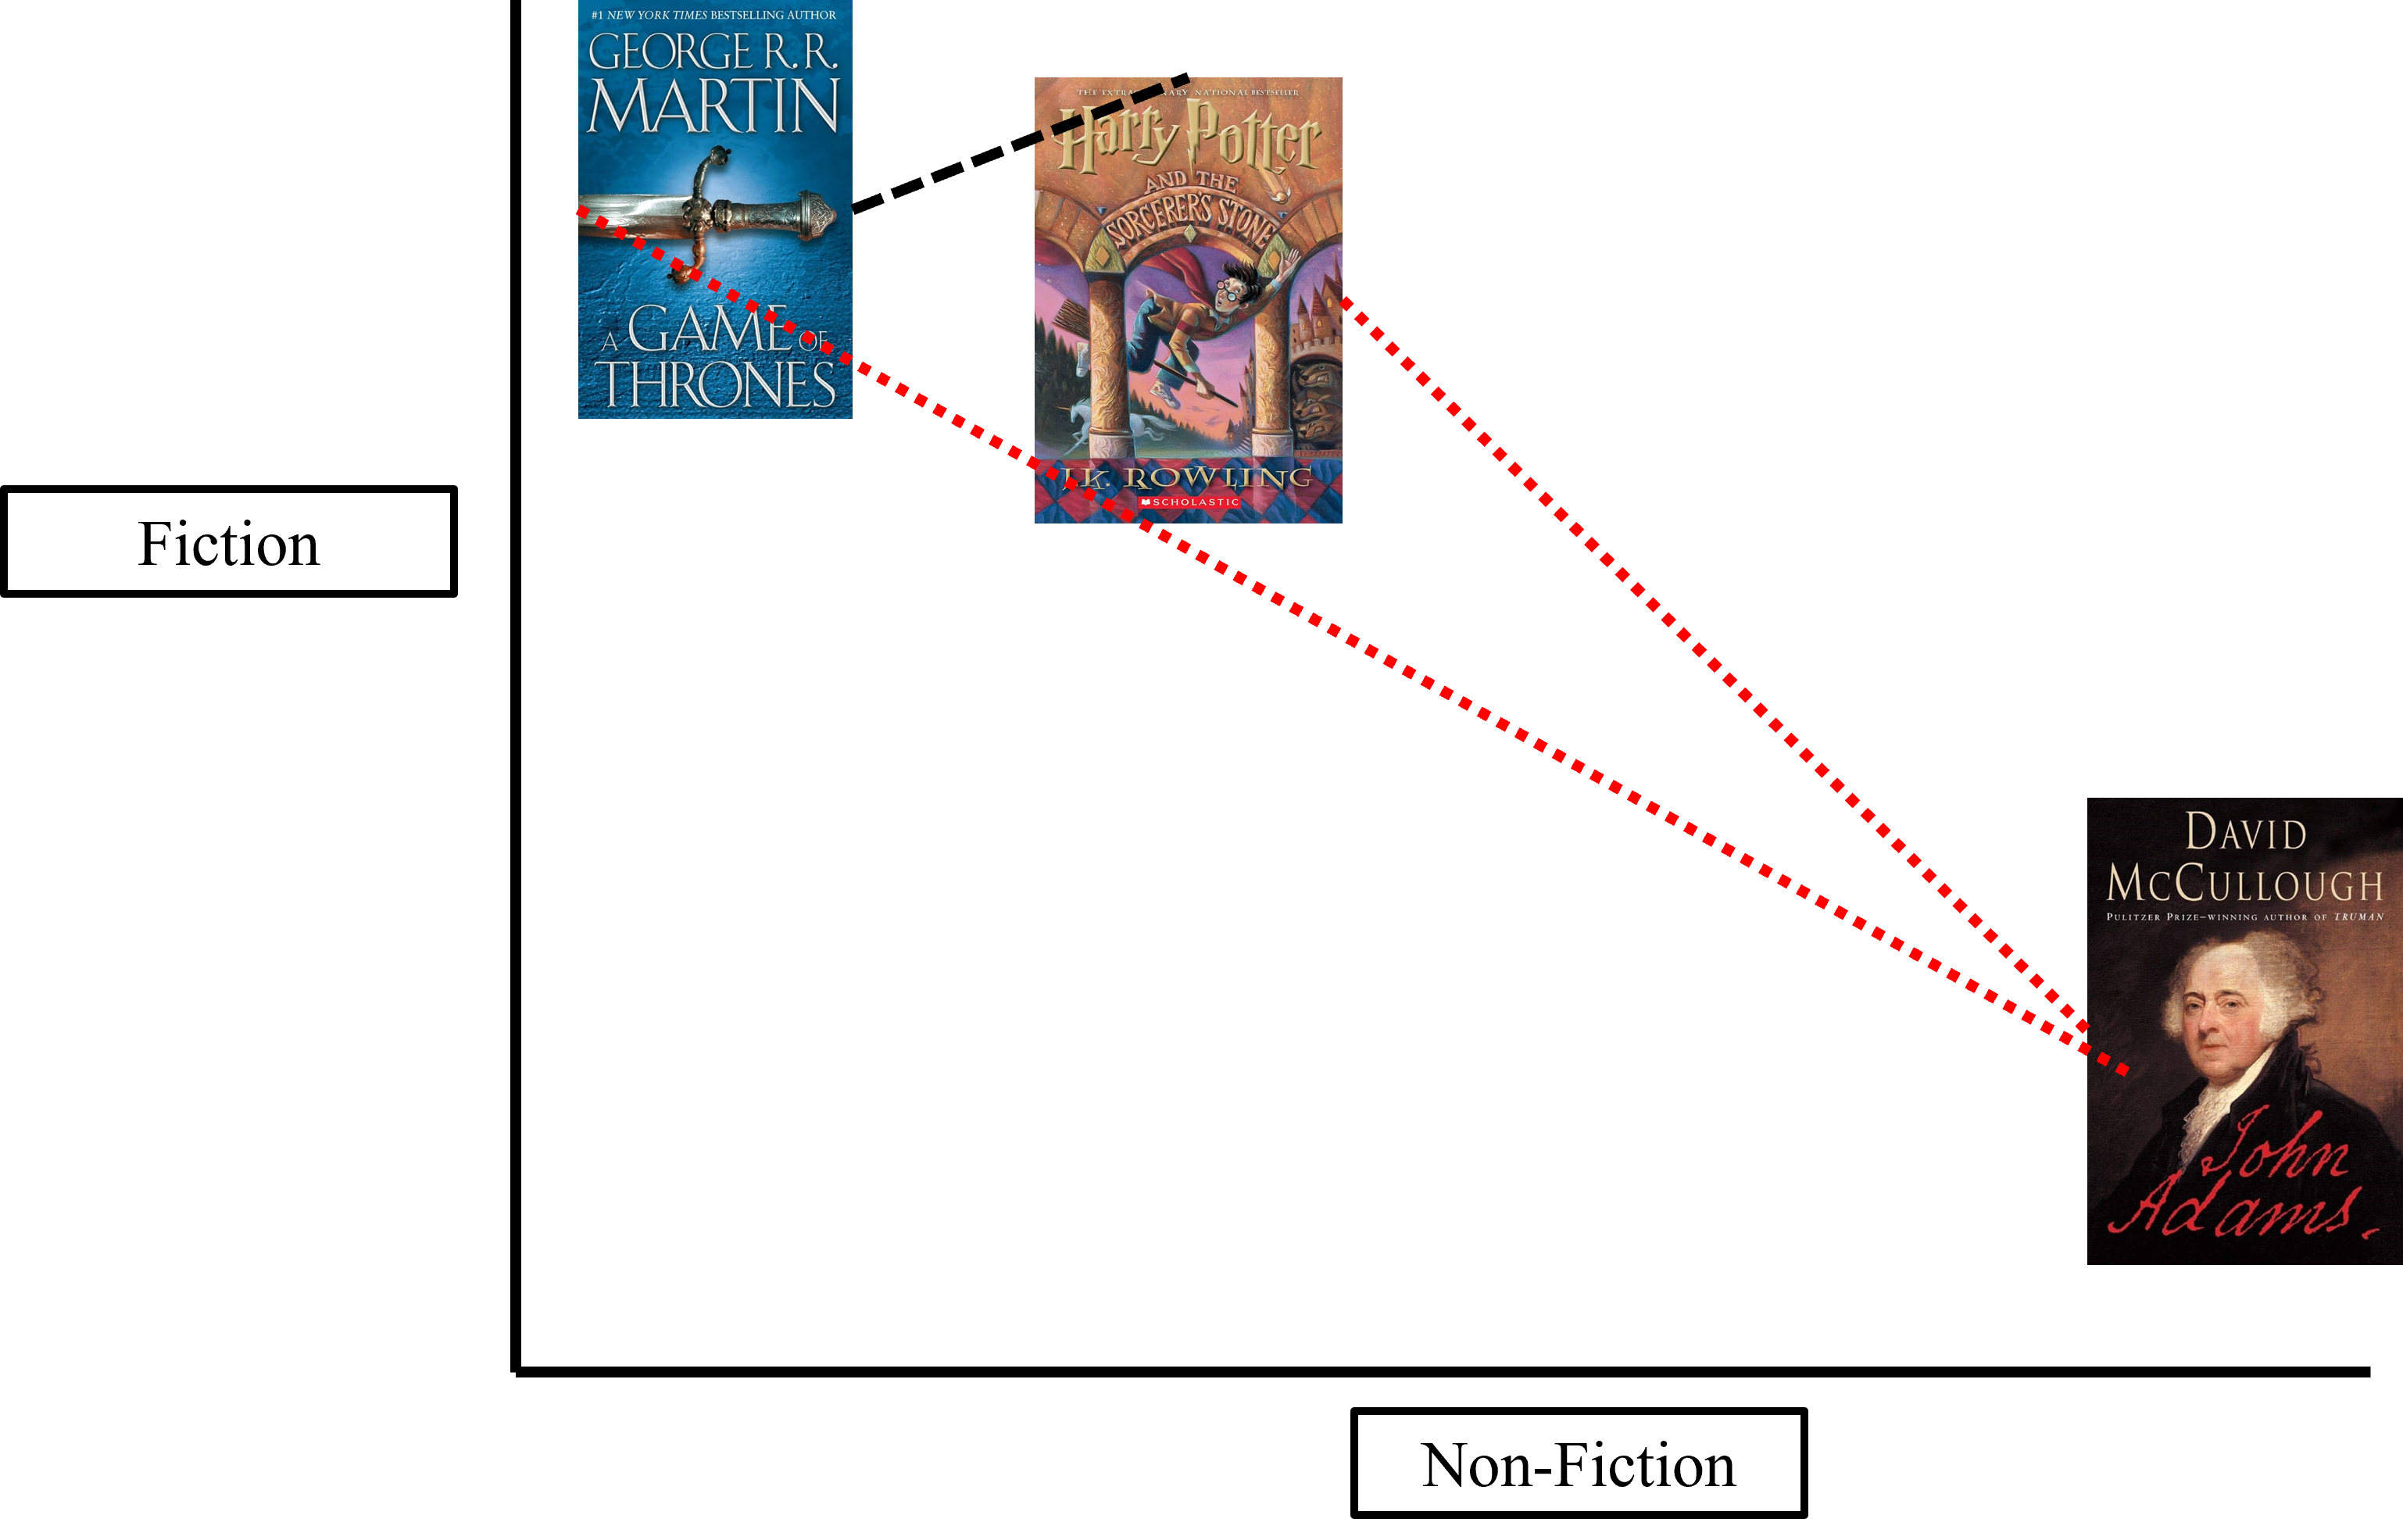
\includegraphics[width=0.55\textwidth]{../supplemental_materials/library_13.png}
\end{figure}
\end{frame}

\section{Estimating Embeddings}\label{estimating-embeddings}

\begin{frame}{Estimating Embeddings -- Four Considerations (Rodriguez \&
Spirling 2022)}
\phantomsection\label{estimating-embeddings-four-considerations-rodriguez-spirling-2022}
\begin{enumerate}
\item \textbf{Data Source}: These models generally require (very) large source of text data (ex: Wikipedia) for algorithms to accurately discern patterns and associations.
\par \vspace{2.5mm} \pause

\item \textbf{Content Window Size}: Capturing semantic relationships means we need to understand contextual usage of words. Most of these embedding models are trained to predict words given surrounding text (or visa-versa), so how much text surrounding these \emph{focal} words in training is important. 
\par \vspace{2.5mm} \pause

\item \textbf{Dimension of the Embedding}: Dimensions -- i.e., length of $k$ dense vector -- to represent words. Pre-trained embeddings we will use today are generally low-dimensional spaces (50-500 dimensions). 
\par \vspace{2.5mm} \pause

\item \textbf{Algorithm}: How we execute and optimize the strategy -- i.e., how do we want to recover embeddings from the data? 
\end{enumerate}
\end{frame}

\begin{frame}{Neural Word Embeddings}
\phantomsection\label{neural-word-embeddings}
\begin{itemize}
\item Most modern embedding techniques are derived from \textbf{neural networks} -- computational framework modeled on the synaptic processes of the human brain.  \par \vspace{2.5mm} 
\item They learn patterns through layers of \emph{neurons} -- including \emph{hidden} layers that help the model understand complex relationships \par \vspace{2.5mm} \pause
\item Continuous Bag of Word for \texttt{john adams with the second president of the united states} \par \vspace{2.5mm}
\item[] Focal Word = \texttt{president}:  $\operatorname*{arg\,max}_{\mu_{\text{president}}} = \frac{\exp(\mu_{\text{president}}\cdot\overline{v})}{\sum_{j}\exp(\mu_{j}\cdot\overline{v})}$ \vspace{2.5mm} \par 
\item Where $\overline{v}$ represents the average of all embeddings for words in the string other than `president`, while $j$ indexes over the entire vocabulary (i.e., every other token available in the corpus -- not just in current sentence).
\end{itemize}
\end{frame}

\section{Pre-Trained Embeddings}\label{pre-trained-embeddings}

\begin{frame}{Pre-Trained Embeddings}
\phantomsection\label{pre-trained-embeddings-1}
\begin{itemize}
\item Training these models are incredibly burdensome -- lots of data needed and computationally intensive! \par \vspace{2.5mm}
\item Instead, we often rely on pre-trained embeddings that we can use to locate specific text for our own application  \par \vspace{2.5mm}
\item We're going to focus on three: \texttt{word2vec}, \texttt{GloVe}, and \texttt{BERT}
\end{itemize}
\end{frame}

\begin{frame}{word2vec}
\phantomsection\label{word2vec}
\begin{itemize}
\item Developed by \texttt{Google} in 2023.  \par \vspace{2.5mm}
\item Trained using text from \texttt{Google News} ($\approx$ 100 billion words) \par \vspace{2.5mm}
\item Follows intuition of Continuous Bag of Words (COBW) \& negative sampling to predict a focal word.  \par \vspace{2.5mm}
\item We'll first use \texttt{word2vec} to predict a CBOW model. 
\end{itemize}
\end{frame}

\begin{frame}[fragile]{word2vec (Cont.)}
\phantomsection\label{word2vec-cont.}
\scriptsize

\begin{Shaded}
\begin{Highlighting}[]
\FunctionTok{library}\NormalTok{(word2vec) }\CommentTok{\# Load Package}

\NormalTok{reviews }\OtherTok{=} \FunctionTok{sapply}\NormalTok{(imdb, reduce\_complexity) }\CommentTok{\# Text from IMDB Reviews Dataset}

\NormalTok{cbow\_model }\OtherTok{=} \FunctionTok{word2vec}\NormalTok{(}\AttributeTok{x =}\NormalTok{ reviews, }\CommentTok{\# IMDB Text}
                      \AttributeTok{type =} \StringTok{"cbow"}\NormalTok{, }\CommentTok{\# Cont. Bag of Words }
                      \AttributeTok{dim =} \DecValTok{15}\NormalTok{, }\CommentTok{\# 15 Dimensions}
                      \AttributeTok{iter =} \DecValTok{20}\NormalTok{) }\CommentTok{\# 20 Iterations (max)}
\end{Highlighting}
\end{Shaded}
\end{frame}

\begin{frame}[fragile]{word2vec (Nearest Words)}
\phantomsection\label{word2vec-nearest-words}
\scriptsize

\begin{Shaded}
\begin{Highlighting}[]
\NormalTok{cbow\_lookslike }\OtherTok{\textless{}{-}} \FunctionTok{predict}\NormalTok{(cbow\_model, }\FunctionTok{c}\NormalTok{(}\StringTok{"terrible"}\NormalTok{, }\StringTok{"incredible"}\NormalTok{), }\AttributeTok{type =} \StringTok{"nearest"}\NormalTok{, }\AttributeTok{top\_n =} \DecValTok{5}\NormalTok{)}
\FunctionTok{print}\NormalTok{(cbow\_lookslike)}
\end{Highlighting}
\end{Shaded}

\begin{verbatim}
$terrible
     term1    term2 similarity rank
1 terrible   redeem  0.9385457    1
2 terrible   insult  0.9331042    2
3 terrible   stupid  0.9115961    3
4 terrible dialogue  0.9073911    4
5 terrible  express  0.8999336    5

$incredible
       term1     term2 similarity rank
1 incredible inventive  0.9537759    1
2 incredible   impress  0.9290549    2
3 incredible    makeup  0.9229119    3
4 incredible effective  0.9174616    4
5 incredible   bravery  0.9123820    5
\end{verbatim}
\end{frame}

\begin{frame}[fragile]{word2vec (Embeddings Themselves!)}
\phantomsection\label{word2vec-embeddings-themselves}
\scriptsize

\begin{Shaded}
\begin{Highlighting}[]
\NormalTok{cbow\_embedding }\OtherTok{\textless{}{-}} \FunctionTok{predict}\NormalTok{(cbow\_model, }\FunctionTok{c}\NormalTok{(}\StringTok{"terrible"}\NormalTok{, }\StringTok{"incredible"}\NormalTok{),}\AttributeTok{type =} \StringTok{"embedding"}\NormalTok{)}
\FunctionTok{print}\NormalTok{(cbow\_embedding)}
\end{Highlighting}
\end{Shaded}

\begin{verbatim}
                [,1]       [,2]       [,3]       [,4]       [,5]       [,6]       [,7]       [,8]       [,9]     [,10]
terrible   -1.481836 -0.3323868 -0.3105061 -0.3843328 0.25146413 -0.2309697 -0.9046581  1.4401903 -2.5360181 0.6599042
incredible -0.520224  0.7336361 -1.1396466 -0.3880426 0.07553662 -1.0354885 -0.7040370 -0.1177941 -0.2107209 1.6104442
               [,11]     [,12]      [,13]      [,14]      [,15]
terrible   0.9010985 0.4093859 -0.9944206 -0.3474618 -0.6959757
incredible 0.4362197 0.5286055 -1.7181001  1.9030302 -1.2137759
\end{verbatim}
\end{frame}

\begin{frame}[fragile]{word2vec (Visualize Embedding Space)}
\phantomsection\label{word2vec-visualize-embedding-space}
\scriptsize

\begin{Shaded}
\begin{Highlighting}[]
\NormalTok{word\_vectors }\OtherTok{\textless{}{-}} \FunctionTok{as.matrix}\NormalTok{(cbow\_model) }\CommentTok{\# Convert Model to Matrix}
\NormalTok{similar\_words }\OtherTok{\textless{}{-}} \FunctionTok{unique}\NormalTok{(}\FunctionTok{c}\NormalTok{(}\FunctionTok{c}\NormalTok{(}\StringTok{"terrible"}\NormalTok{, }\StringTok{"incredible"}\NormalTok{) , }\FunctionTok{unlist}\NormalTok{(}\FunctionTok{predict}\NormalTok{(cbow\_model, }\FunctionTok{c}\NormalTok{(}\StringTok{"terrible"}\NormalTok{, }\StringTok{"incredible"}\NormalTok{) , }\AttributeTok{type =} \StringTok{"nearest"}\NormalTok{, }\AttributeTok{top\_n =} \DecValTok{10}\NormalTok{))))}
\NormalTok{word\_vec\_subset }\OtherTok{\textless{}{-}}\NormalTok{ word\_vectors[}\FunctionTok{rownames}\NormalTok{(word\_vectors) }\SpecialCharTok{\%in\%}\NormalTok{ similar\_words, ] }\CommentTok{\# Filter to Similar Words}

\FunctionTok{set.seed}\NormalTok{(}\DecValTok{123}\NormalTok{) }\CommentTok{\# Set Random Seed}

\NormalTok{tsne\_out }\OtherTok{\textless{}{-}} \FunctionTok{invisible}\NormalTok{(}\FunctionTok{Rtsne}\NormalTok{(}
\NormalTok{  word\_vec\_subset, }\CommentTok{\# Subset of Similar Words}
  \AttributeTok{dims =} \DecValTok{2}\NormalTok{,  }\CommentTok{\# 2 Dimensions}
  \AttributeTok{perplexity =} \DecValTok{5}\NormalTok{, }
  \AttributeTok{verbose =} \ConstantTok{FALSE}\NormalTok{, }
  \AttributeTok{max\_iter =} \DecValTok{500} 
\NormalTok{)) }
\end{Highlighting}
\end{Shaded}
\end{frame}

\begin{frame}{word2vec (Visualize Embedding Space - Cont.)}
\phantomsection\label{word2vec-visualize-embedding-space---cont.}
\begin{center}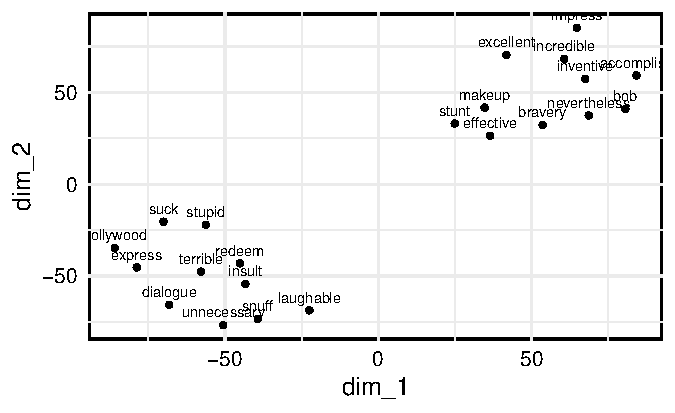
\includegraphics{class_9_embeddings_files/figure-beamer/word2vec_5-1} \end{center}
\end{frame}

\begin{frame}{word2vec}
\phantomsection\label{word2vec-1}
\begin{itemize}
\item Your turn -- Pick two random words and re-create the analysis. 
\end{itemize}
\end{frame}

\begin{frame}{GLoVe}
\phantomsection\label{glove}
\begin{itemize}
\item \texttt{word2vec}: \emph{I’ll look at the words around this word and try to guess it} (\textbf{local prediction}) \par \vspace{2.5mm} \pause
\item \texttt{GloVe}: \emph{I’ll look at how often this word co-occurs with all other words in the corpus} (\textbf{global statistics}) \par \vspace{2.5mm} \pause
\item Developed by researchers at Stanford -- combines text from Wikipedia (4.5 billion tokens), Gigaword (6 billion), and Common Crawl (100s Billions) \par \vspace{2.5mm} \pause
\item Process: Factorizes a word co-occurrence matrix from the entire available corpus, such that each word has its own vector but can also recover entire corpus statistics (not just insight from small context windows)
\end{itemize}
\end{frame}

\begin{frame}[fragile]{GloVe (Cont.)}
\phantomsection\label{glove-cont.}
\begin{itemize}
\item Unlike \texttt{word2vec} -- you need to download \texttt{GloVe} (varying model sizes) to run in \texttt{R}
\item Once loaded -- we can use it to recover cosine similarity of words
\end{itemize}
\scriptsize

\begin{Shaded}
\begin{Highlighting}[]
\NormalTok{glove\_mat }\OtherTok{\textless{}{-}} \FunctionTok{as.matrix}\NormalTok{(glove[, }\SpecialCharTok{{-}}\DecValTok{1}\NormalTok{]) }\CommentTok{\# Convert Glove to Matrix}
\FunctionTok{rownames}\NormalTok{(glove\_mat) }\OtherTok{\textless{}{-}}\NormalTok{ glove}\SpecialCharTok{$}\NormalTok{word }\CommentTok{\# Assign Rownames}

\NormalTok{words }\OtherTok{\textless{}{-}} \FunctionTok{c}\NormalTok{(}\StringTok{\textquotesingle{}dog\textquotesingle{}}\NormalTok{, }\StringTok{\textquotesingle{}cat\textquotesingle{}}\NormalTok{, }\StringTok{\textquotesingle{}horse\textquotesingle{}}\NormalTok{, }\StringTok{\textquotesingle{}pig\textquotesingle{}}\NormalTok{, }\StringTok{\textquotesingle{}firetruck\textquotesingle{}}\NormalTok{) }\CommentTok{\# Words}

\NormalTok{cosine\_similarity }\OtherTok{\textless{}{-}} \ControlFlowTok{function}\NormalTok{(u, v) \{}
  \FunctionTok{sum}\NormalTok{(u}\SpecialCharTok{*}\NormalTok{v) }\SpecialCharTok{/}\NormalTok{ (}\FunctionTok{sqrt}\NormalTok{(}\FunctionTok{sum}\NormalTok{(u}\SpecialCharTok{\^{}}\DecValTok{2}\NormalTok{)) }\SpecialCharTok{*} \FunctionTok{sqrt}\NormalTok{(}\FunctionTok{sum}\NormalTok{(v}\SpecialCharTok{\^{}}\DecValTok{2}\NormalTok{)))}
\NormalTok{\} }\CommentTok{\# Function to Recove Cosine Sim}
\end{Highlighting}
\end{Shaded}
\end{frame}

\begin{frame}[fragile]{GloVe (Cont.)}
\phantomsection\label{glove-cont.-1}
\scriptsize

\begin{Shaded}
\begin{Highlighting}[]
\NormalTok{n }\OtherTok{=} \FunctionTok{length}\NormalTok{(words)}
\NormalTok{cosine\_sim\_matrix }\OtherTok{\textless{}{-}} \FunctionTok{matrix}\NormalTok{(}\AttributeTok{nrow =}\NormalTok{ n, }\AttributeTok{ncol =}\NormalTok{ n)}
\FunctionTok{colnames}\NormalTok{(cosine\_sim\_matrix) }\OtherTok{\textless{}{-}} \FunctionTok{rownames}\NormalTok{(cosine\_sim\_matrix) }\OtherTok{\textless{}{-}}\NormalTok{ words}

\ControlFlowTok{for}\NormalTok{ (i }\ControlFlowTok{in} \DecValTok{1}\SpecialCharTok{:}\FunctionTok{length}\NormalTok{(words))\{}
\NormalTok{  temp\_word }\OtherTok{\textless{}{-}}\NormalTok{ words[i]}
  \ControlFlowTok{for}\NormalTok{ (j }\ControlFlowTok{in} \DecValTok{1}\SpecialCharTok{:}\FunctionTok{length}\NormalTok{(words))\{}
\NormalTok{    temp\_comparison\_word }\OtherTok{\textless{}{-}}\NormalTok{ words[j]}
\NormalTok{    cosine\_sim\_matrix[i, j] }\OtherTok{\textless{}{-}} \FunctionTok{cosine\_similarity}\NormalTok{(}\AttributeTok{u =}\NormalTok{ glove\_mat[}\FunctionTok{as.character}\NormalTok{(temp\_word), ], }
                                         \AttributeTok{v =}\NormalTok{ glove\_mat[}\FunctionTok{as.character}\NormalTok{(temp\_comparison\_word), ])}
\NormalTok{    \} }\CommentTok{\# Recover Cosine Sim }
\NormalTok{\} }\CommentTok{\# Recover Cosine Sim for Each Word Pair}
\end{Highlighting}
\end{Shaded}
\end{frame}

\begin{frame}{GloVe (Cont.)}
\phantomsection\label{glove-cont.-2}
\scriptsize

\begin{center}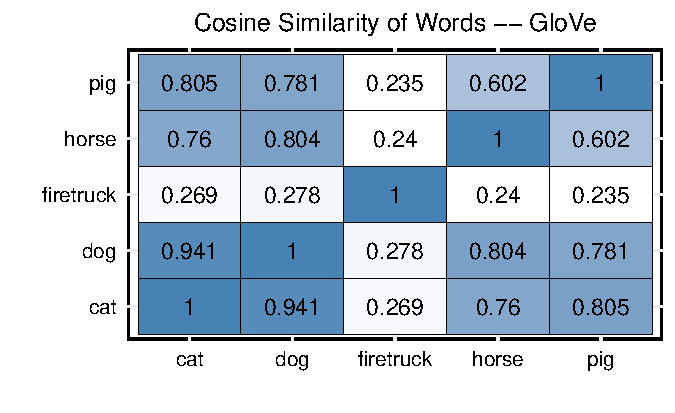
\includegraphics{class_9_embeddings_files/figure-beamer/glove_3-1} \end{center}
\end{frame}

\begin{frame}{BERT (Bidirectional Encoder Representations from
Transformers)}
\phantomsection\label{bert-bidirectional-encoder-representations-from-transformers}
\begin{itemize}
\item Part of the \textbf{transformer revolution}: Uses bidirectional attention in a masked language model for next sentence prediction to learn context-dependent word and sentence representations. \par \vspace{2.5mm} \pause
\item In short... masked language step teaches the model the meaning of each word in context (i.e., encoding), while the next sentence predictions step teaches the model how sentences fit together logically.  \par \vspace{2.5mm} \pause
\item \textbf{Different from Nueral Networks}: They process sequentially -- while the bi-directional attention mechanisms for transformer-based models let each word consider all other words at once!  \par \vspace{2.5mm}
\item Result: An output vector that isn’t static like \texttt{word2vec} or \texttt{GloVe}, but a context-based embedding that changes depending on how words are used.
\end{itemize}
\end{frame}

\begin{frame}[fragile]{BERT -- Apply Using Python Code (Reticulate)}
\phantomsection\label{bert-apply-using-python-code-reticulate}
\scriptsize

\begin{Shaded}
\begin{Highlighting}[]
\FunctionTok{library}\NormalTok{(reticulate) }\CommentTok{\# Activate Reticulate}
\FunctionTok{virtualenv\_create}\NormalTok{()}\CommentTok{\# Create  Virtual Environment (If Needed)}
\end{Highlighting}
\end{Shaded}

\begin{verbatim}
virtualenv: ~/.virtualenvs/r-reticulate
\end{verbatim}

\begin{Shaded}
\begin{Highlighting}[]
\FunctionTok{use\_virtualenv}\NormalTok{(}\AttributeTok{required =} \ConstantTok{TRUE}\NormalTok{) }\CommentTok{\# Activate Environment}

\NormalTok{required\_packages }\OtherTok{\textless{}{-}} \FunctionTok{c}\NormalTok{(}\StringTok{"torch"}\NormalTok{, }\StringTok{"transformers"}\NormalTok{, }\StringTok{"sentence{-}transformers"}\NormalTok{)}
\ControlFlowTok{for}\NormalTok{ (pkg }\ControlFlowTok{in}\NormalTok{ required\_packages) \{}
  \ControlFlowTok{if}\NormalTok{ (}\SpecialCharTok{!}\FunctionTok{py\_module\_available}\NormalTok{(pkg)) \{}
    \FunctionTok{virtualenv\_install}\NormalTok{(}\AttributeTok{packages =}\NormalTok{ pkg)}
\NormalTok{  \}}
\NormalTok{\} }\CommentTok{\# Install torch, transformers, and sentence{-}transformers (if needed)}
\end{Highlighting}
\end{Shaded}

\begin{verbatim}
Using virtual environment "~/.virtualenvs/r-reticulate" ...
\end{verbatim}

\begin{verbatim}
+ "C:/Users/jaketruscott/Documents/.virtualenvs/r-reticulate/Scripts/python.exe" -m pip install --upgrade --no-user sentence-transformers
\end{verbatim}
\end{frame}

\begin{frame}[fragile]{BERT -- Apply Using Python Code (Cont.)}
\phantomsection\label{bert-apply-using-python-code-cont.}
\scriptsize

\begin{Shaded}
\begin{Highlighting}[]
\NormalTok{sentence\_transformers }\OtherTok{\textless{}{-}} \FunctionTok{import}\NormalTok{(}\StringTok{"sentence\_transformers"}\NormalTok{) }\CommentTok{\# Import sentence{-}transformers}
\NormalTok{model }\OtherTok{\textless{}{-}}\NormalTok{ sentence\_transformers}\SpecialCharTok{$}\FunctionTok{SentenceTransformer}\NormalTok{(}\StringTok{"all{-}MiniLM{-}L6{-}v2"}\NormalTok{) }\CommentTok{\# Call Small Bert Model}

\NormalTok{words }\OtherTok{\textless{}{-}} \FunctionTok{c}\NormalTok{(}\StringTok{\textquotesingle{}dog\textquotesingle{}}\NormalTok{, }\StringTok{\textquotesingle{}cat\textquotesingle{}}\NormalTok{, }\StringTok{\textquotesingle{}horse\textquotesingle{}}\NormalTok{, }\StringTok{\textquotesingle{}pig\textquotesingle{}}\NormalTok{, }\StringTok{\textquotesingle{}firetruck\textquotesingle{}}\NormalTok{)}\CommentTok{\# Same Words as Earlier}
\NormalTok{embeddings }\OtherTok{\textless{}{-}}\NormalTok{ model}\SpecialCharTok{$}\FunctionTok{encode}\NormalTok{(words) }\CommentTok{\# Recover Embeddings}

\NormalTok{n }\OtherTok{\textless{}{-}} \FunctionTok{length}\NormalTok{(words)}
\NormalTok{cosine\_sim\_matrix }\OtherTok{\textless{}{-}} \FunctionTok{matrix}\NormalTok{(}\AttributeTok{nrow =} \FunctionTok{length}\NormalTok{(words), }\AttributeTok{ncol =} \FunctionTok{length}\NormalTok{(words))}
\FunctionTok{rownames}\NormalTok{(cosine\_sim\_matrix) }\OtherTok{\textless{}{-}} \FunctionTok{colnames}\NormalTok{(cosine\_sim\_matrix) }\OtherTok{\textless{}{-}}\NormalTok{ words}

\ControlFlowTok{for}\NormalTok{ (i }\ControlFlowTok{in} \DecValTok{1}\SpecialCharTok{:}\NormalTok{n) \{}
  \ControlFlowTok{for}\NormalTok{ (j }\ControlFlowTok{in} \DecValTok{1}\SpecialCharTok{:}\NormalTok{n) \{}
\NormalTok{    cosine\_sim\_matrix[i, j] }\OtherTok{\textless{}{-}} \FunctionTok{cosine\_similarity}\NormalTok{(embeddings[i, ], embeddings[j, ])}
\NormalTok{  \}}
\NormalTok{\} }\CommentTok{\# Recover Cosine Sim for Each Word Pair}
\end{Highlighting}
\end{Shaded}
\end{frame}

\begin{frame}{BERT -- Same Application as Glove But Context-Specific
Results!}
\phantomsection\label{bert-same-application-as-glove-but-context-specific-results}
\scriptsize

\begin{center}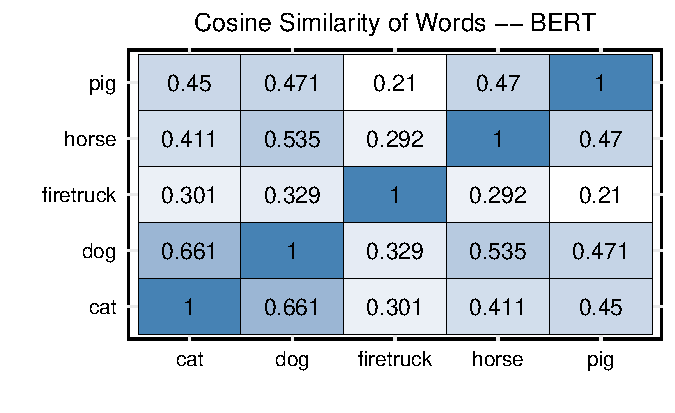
\includegraphics{class_9_embeddings_files/figure-beamer/bert_3-1} \end{center}
\end{frame}

\section{Looking Forward}\label{looking-forward}

\begin{frame}{Next Class}
\phantomsection\label{next-class}
\begin{itemize}
\item Last substantive class before presentations! 
\item Text-Based Models for Measuring Ideology
\item \textbf{Remember}: Optional paper drafts due via email on \textbf{4/3}
\end{itemize}
\end{frame}

\end{document}
